%%%%%%%%%%%%%%%%%%%%%%%%%%%%%%%%%%%%%%%%%%%%%%%%%%%%%%%
%%%%%%%%%%%%%%%%%%%%%%%%%%%%%%%%%%%%%%%%%%%%%%%%%%%%%%%

% The High-Granularity Calorimeter and HGCROC

% Description of the HL-LHC phase
% What are the main changes in the CMS detector that are expected for the HL-LHC?
% Description of the High-Granularity Calorimeter
% The read-out structure and HGCROC
% Description of HGCROC
% How can you characterize the chip?
% The irradiation test: TID and SEE
% Improvements in the chip design
% Conclusion

%%%%%%%%%%%%%%%%%%%%%%%%%%%%%%%%%%%%%%%%%%%%%%%%%%%%%%%
%%%%%%%%%%%%%%%%%%%%%%%%%%%%%%%%%%%%%%%%%%%%%%%%%%%%%%%

\chapter{The CMS Endcap Calorimeter Upgrade}
\label{chapter:The CMS Endcap Calorimeter Upgrade}

After nearly fifteen years of dedicated service, the LHC will undergo a major upgrade towards the High Luminosity LHC phase (HL-LHC), which is expected to start its operations by the end of 2029.
The upgraded machine has been designed to operate at a  centre-of-mass energy of 14~TeV and to achieve a peak instantaneous luminosity of $L=5\cdot10^{34}\;cm^{-2}s^{-1}$: in these unprecedented running conditions, a remarkable integrated luminosity of 4000~$fb^{-1}$ is expected to be collected over the anticipated ten years of data-taking. 
With the HL-LHC upgrade, the amount of collected data will significantly increase, so as the potential for new discoveries at the LHC. The increased statistics will allow for more precise measurements of the SM properties but will also improve the potential for new discoveries, enhance the sensitivity to rare processes and possibly unveil the presence of previously unknown particles and BSM scenarios.

The higher luminosities of the HL-LHC will also result in exceedingly high pile-up rates, with $\mathcal{O}(200)$ events per bunch crossing and unprecedented radiation levels, with fluences of up to $3.5\times10^6\,\textrm{s}^{-1}\,\textrm{cm}^{-2}$ and a total absorbed dose of up to $\sim$$200\,\textrm{Mrad}$, thus posing several technical challenges for the operation of the detectors and the entire infrastructure.
In order to maintain its excellent physics performance in the high pile-up environment of the HL-LHC, the CMS Collaboration, as well as the other LHC experiments, is planning a series of major upgrades of the sub-detectors. The upgrade development and realization has already started during the Second Long Shutdown (LS2, 2018-2022) and will continue in the Third Long Shutdown (LS3, 2025-2029) when the installation and commissioning of the new detectors will be performed. 

\bigbreak

In this chapter, after a brief overview of the CMS upgrade plans in Sec.~\ref{sec:Upgrades of the CMS detector}, the focus will be directed towards the High Granularity Calorimeter (HGCAL), that will replace the current endcap calorimeters and completely renovate the CMS forward calorimetry strategy. The HGCAL detector, described in Sec.\ref{sec:The High-Granularity Calorimeter design} will provide the very first large-scale silicon-based imaging calorimeter employed in a high-energy physics experiment, with extremely fine transverse and longitudinal granularity, including a total of 6 million channels. Besides the unprecedented read-out segmentation, the performance requirements for the front-end electronics will be extremely stringent thus calling for ad-hoc electronics development. With an excellent technical effort to meet all these requirements, the HGCROC3 is the final version of the ASIC specifically designed to read-out the modules of the future HGCAL. 
The characteristics of the HGCROC will be described in Sec.~\ref{sec:The HGCAL Front-End Electronics}, while Sec.~\ref{FIXME} will present the irradiation campaigns performed on the chip to test its radiation hardness. 

%%%%%%%%%%%%%%%%%%%%%%%%%%%%%%%%%%%%%%%%%%%%%%%%%%%%%%%%%%%%%%%%%%%%%%%%%%%%%%%%%%%%%%%%%%%%
%%%%%%%%%%%%%%%%%%%%%%%%%%%%%%%%%%%%%%%%%%%%%%%%%%%%%%%%%%%%%%%%%%%%%%%%%%%%%%%%%%%%%%%%%%%%
%%%%%%%%%%%%%%%%%%%%%%%%%%%%%%%%%%%%%%%%%%%%%%%%%%%%%%%%%%%%%%%%%%%%%%%%%%%%%%%%%%%%%%%%%%%%
%%%%%%%%%%%%%%%%%%%%%%%%%%%%%%%%%%%%%%%%%%%%%%%%%%%%%%%%%%%%%%%%%%%%%%%%%%%%%%%%%%%%%%%%%%%%

\section{Upgrades of the CMS detector}
\label{sec:Upgrades of the CMS detector}

In the context of the future HL-LHC phase (Phase-2), the CMS detector upgrades programme has the main objective of maintaining the current physics performance under a new unprecedentedly complex environment. 
After years of operations, many current detector components have become inadequate to withstand high luminosity conditions and will either go through a complete replacement or a significant upgrade of already existing modules. There are three main points the CMS Collaboration has to consider to ensure that the detector's capabilities align with the ambitious research goals of the HL-LHC era:
\begin{itemize}
    \item [-] The unprecedented radiation doses will necessitate a complete replacement of the tracker and endcap calorimeter systems, the adoption of new technologies for the electromagnetic barrel (EB), and substantial enhancements to the electronics systems in the barrel calorimeters and muon detectors.
    \item [-] The increase in the pile-up rate will require highly granular read-outs wherever possible, the implementation of precision timing detectors, and innovative approaches to pile-up mitigation.
    \item [-] The high luminosity will result in an increased data stream, highlighting the crucial need for substantial improvements to the L1 Trigger primitives and the overall Trigger and Data Acquisition System (TriDAS).
\end{itemize}

To enhance the detector's granularity and reconstruction performance while minimizing the material budget, the tracking system will be entirely replaced. This involves employing smaller pixel detectors for the inner tracking system and incorporating strips and macro pixel sensors for the outer tracking stations, extending coverage up to $|\eta|=3.8$. These changes are expected to improve longitudinal and transverse resolutions, as well as reduce fake rates, enabling the reconstruction of L1 trigger tracks up to $|\eta|=2.4$.

The endcap calorimeters will be replaced with the HGCAL, a high-granularity sampling calorimeter designed to enhance shower separation, particle identification, and provide precise timing information.

Additionally, to increase granularity and provide supplementary timing measurements, upgrades to the ECAL and HCAL barrel electronic read-out systems are planned. 

The redundancy of the current muon detection system, comprising DTs, RPCs, and CSCs, will be augmented by the installation of Gas Electron Multiplier chambers and a new generation of RPCs. These enhancements will extend coverage up to $|\eta|=2.8$ and $|\eta|=2.4$, respectively.

Furthermore, multiple MIP timing detectors (MTD) will be positioned in front of the barrel and endcap calorimeters. This additional layer will improve the timing information on charged candidates, which is crucial for disentangling the approximately 200~PU interactions foreseen per bunch crossing.

Finally, the trigger and data acquisition systems will be completely replaced, redesigning the Level-1 hardware trigger to include tracking and high-granularity calorimeter information exploited via the extensive use of state-of-the-art FPGAs and ML techniques.

\bigbreak

Figure~\ref{fig:CMSUpgrade} illustrates a cross-section of the CMS detector, outlining the planned upgrades for the HL-LHC. For each subdetector, the the main modified features are described: the Tracker, TriDAS system and the forward calorimeters will undergo complete replacement, while the MIP timing detector, the barrel calorimeters and the muon system will constitute new parts or modules that are not part of the current CMS design.
% https://cds.cern.ch/record/2628519

\begin{figure}
    \centering
    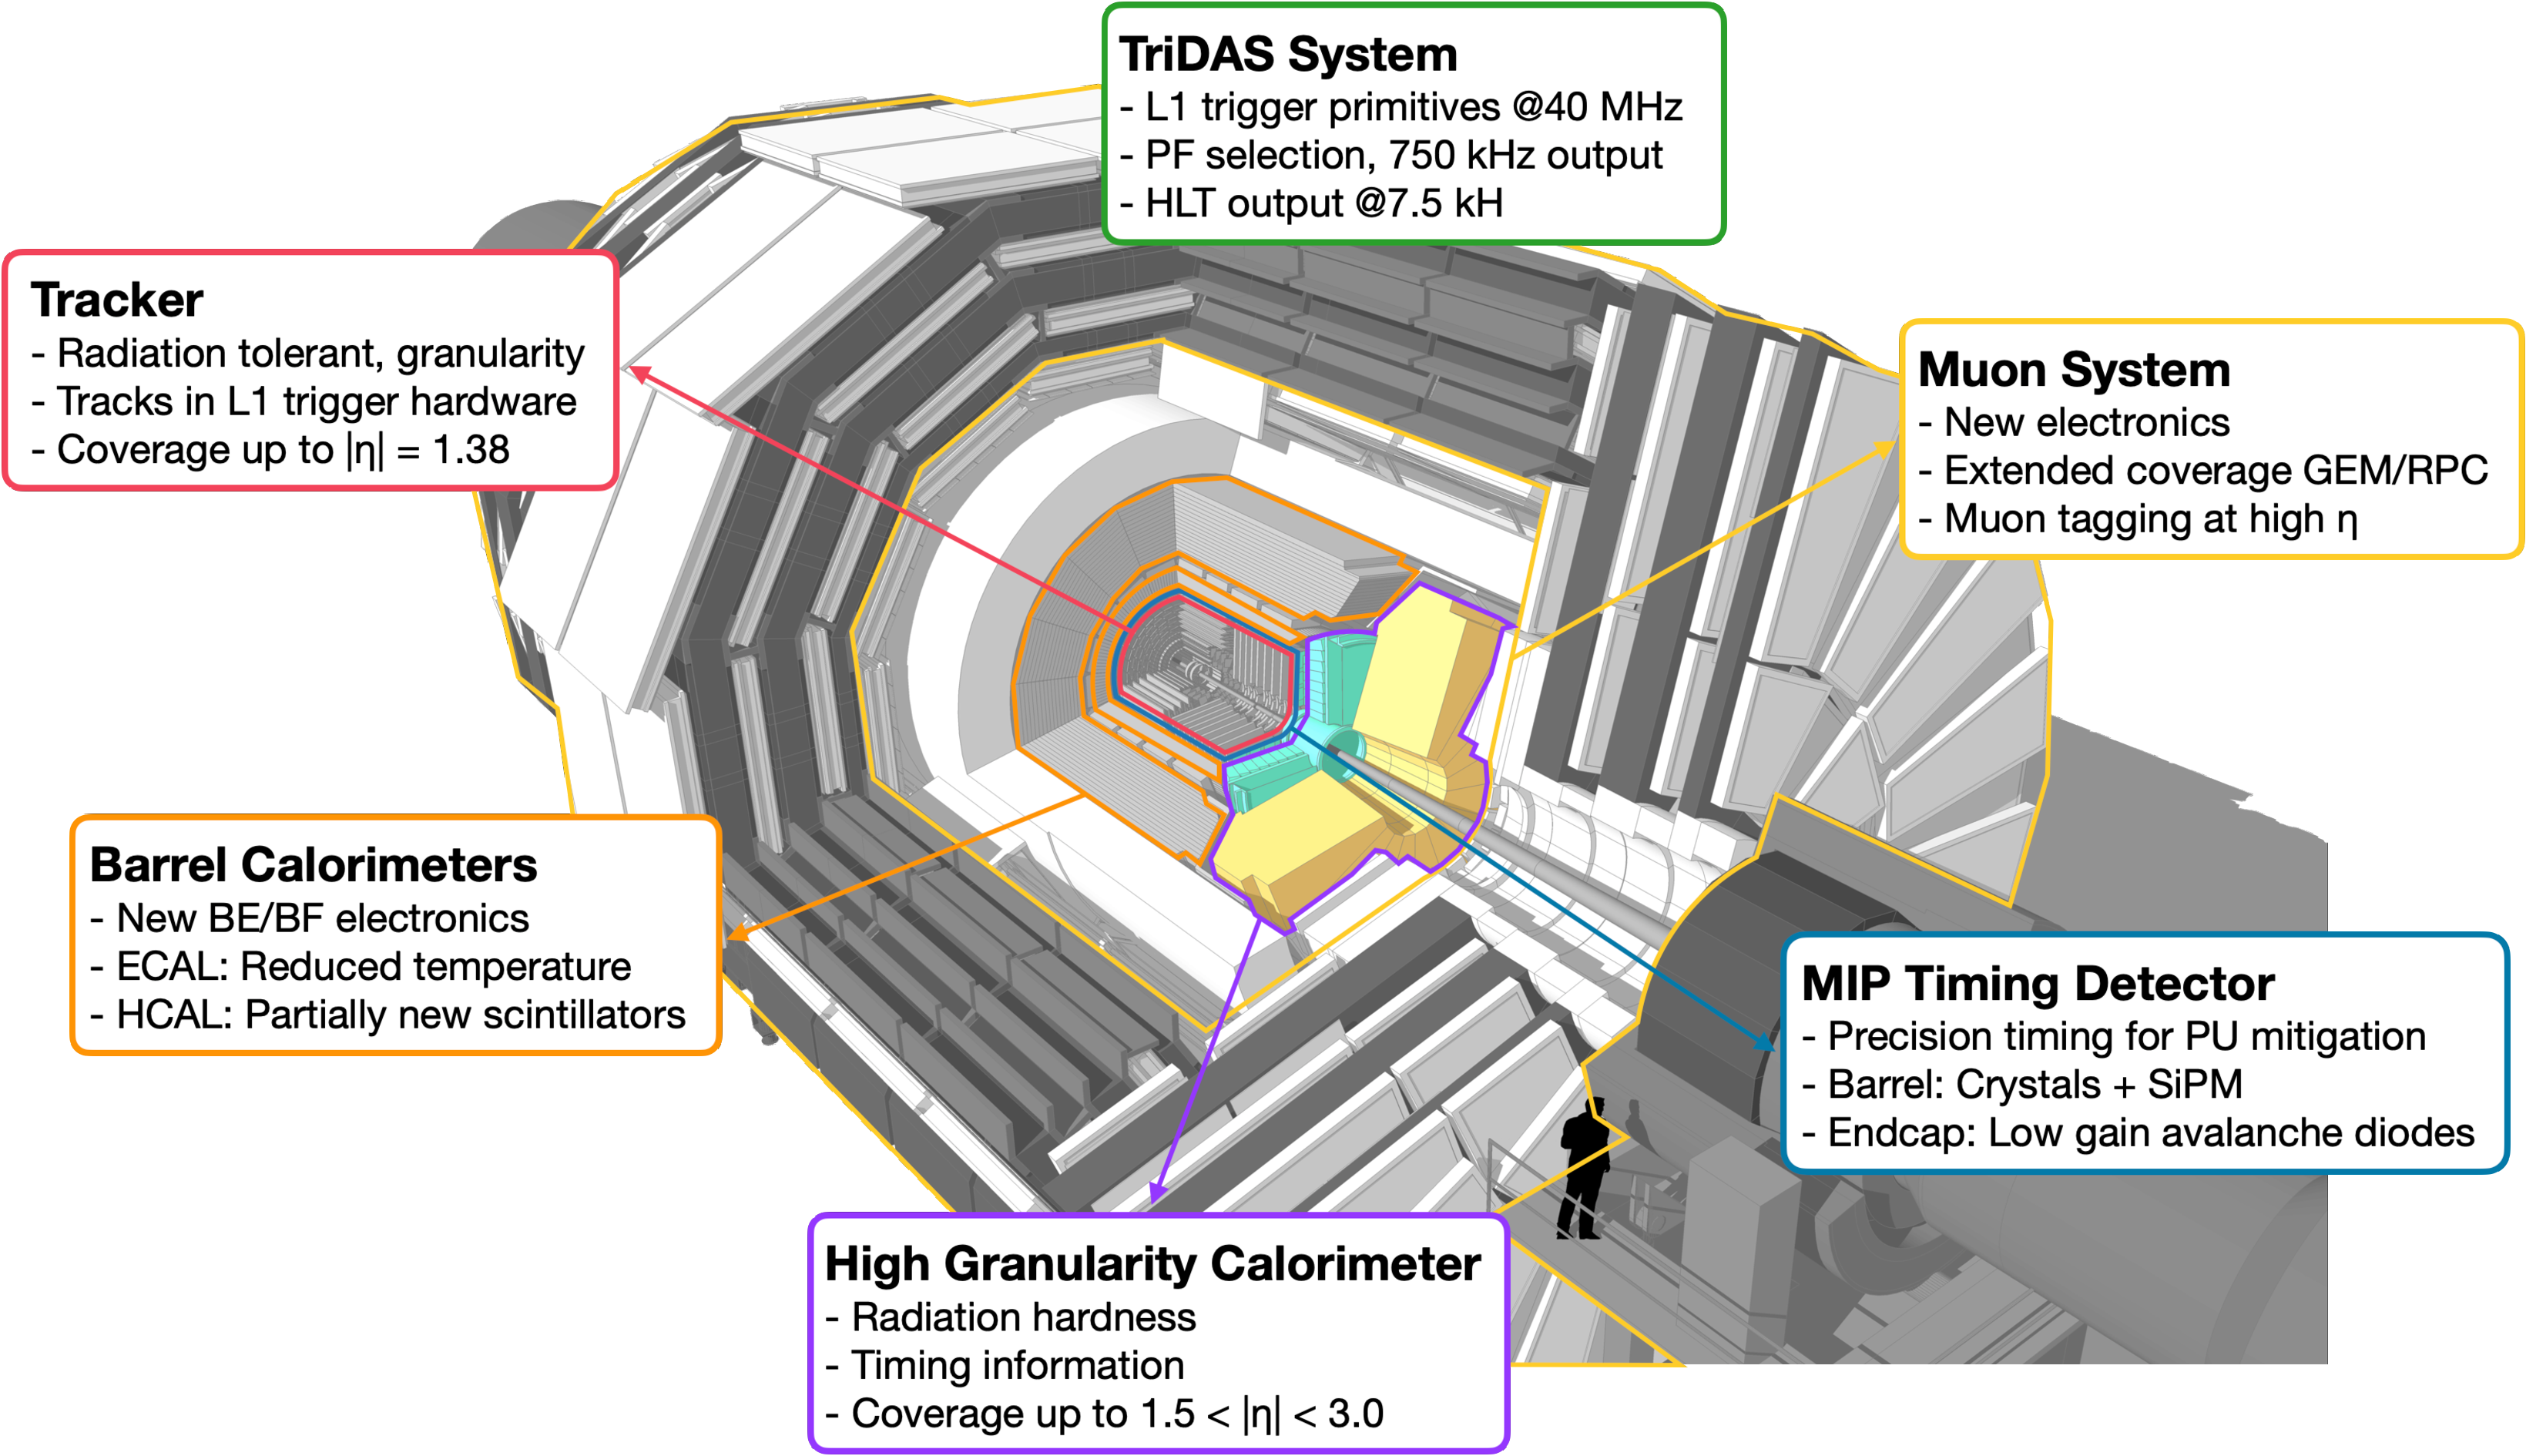
\includegraphics[width=0.95\linewidth]{Figures/HGCAL/CMSUpgrades.pdf}
    \caption{Cross section of the CMS detector with the indication of the upgrades foreseen for the HL-LHC.}
    \label{fig:CMSUpgrade}
\end{figure}

%%%%%%%%%%%%%%%%%%%%%%%%%%%%%%%%%%%%%%%%%%%%%%%%%%%%%%%%%%%%%%%%%%%%%%%%%%%%%%%%%%%%%%%%%%%%
%%%%%%%%%%%%%%%%%%%%%%%%%%%%%%%%%%%%%%%%%%%%%%%%%%%%%%%%%%%%%%%%%%%%%%%%%%%%%%%%%%%%%%%%%%%%
%%%%%%%%%%%%%%%%%%%%%%%%%%%%%%%%%%%%%%%%%%%%%%%%%%%%%%%%%%%%%%%%%%%%%%%%%%%%%%%%%%%%%%%%%%%%
%%%%%%%%%%%%%%%%%%%%%%%%%%%%%%%%%%%%%%%%%%%%%%%%%%%%%%%%%%%%%%%%%%%%%%%%%%%%%%%%%%%%%%%%%%%%

\section{The High-Granularity Calorimeter design}
\label{sec:The High-Granularity Calorimeter design}

Among the CMS detector updates, one of the most ambitious projects is the High Granularity Calorimeter (HGCAL), a high-granularity sampling calorimeter designed to replace the existing CMS endcap calorimeter in order to to maintain a excellent physics performance under the high pile-up and harsh radiation environment of the HL-LHC.

The existing $\textnormal{PbWO}_4$-based Endcap Calorimeters (CE) of the CMS detector were designed to sustain a total integrated luminosity of 500 $\textnormal{fb}^{-1}$. 
The transparency of the lead-tungstate crystals, already degraded during Run-II operations, would not survive the unprecedented radiation flux typical for the HL-LHC environment in this detector region.
It is therefore necessary to replace the current calorimeter endcaps with a new detector with high radiation tolerance, highly granular energy deposit and good time resolution to adequately treat pile-up in the offline event reconstruction. \newline

The HGCAL will consist of 47 layers divided into two compartments:
\begin{itemize}
    \item [-] the Electromagnetic Compartment (CE-E), featuring 26 active layers, interspersed with CuW, Cu, and Pb absorbers,
    \item [-] the Hadronic Compartment (CE-H), composed of 21 layers exploiting stainless steel as passive material.
\end{itemize}

The number of longitudinal samplings has been designed as a trade-off between the best shower reconstruction and the engineering requirements of the mechanical structure. 

To meet the radiation hardness requirements, the CE-E and the front part of the CE-H will employ silicon as active material, for a total area of about 600~$\textnormal{m}^2$ to be covered. In the remaining lower radiation regions of CE-H, at about 4~m from the interaction point, segmented plastic scintillators with silicon photomultipliers (SiPM) for the read-out will be used as the active material. Squared scintillator tiles with sizes ranging from 4~$\textnormal{cm}^2$ up to 30~$\textnormal{cm}^2$ will be installed, for a total of about 400~$\textnormal{m}^2$ of active area covered in scintillators.

This configuration amounts to a total of 10 nuclear radiation lengths ($\lambda_n$), divided into 1.3~$\lambda_n$ for the CE-E and 8.5~$\lambda_n$ for the CE-H. The CE-E alone will extend for a total of 27.7 radiation-lengths ($X_0$).
To further improve radiation resistance, the full system is cooled down to 240~K ($-30^{\circ}$C) with liquid $\textnormal{CO}_2$.

\begin{figure}
    \centering
    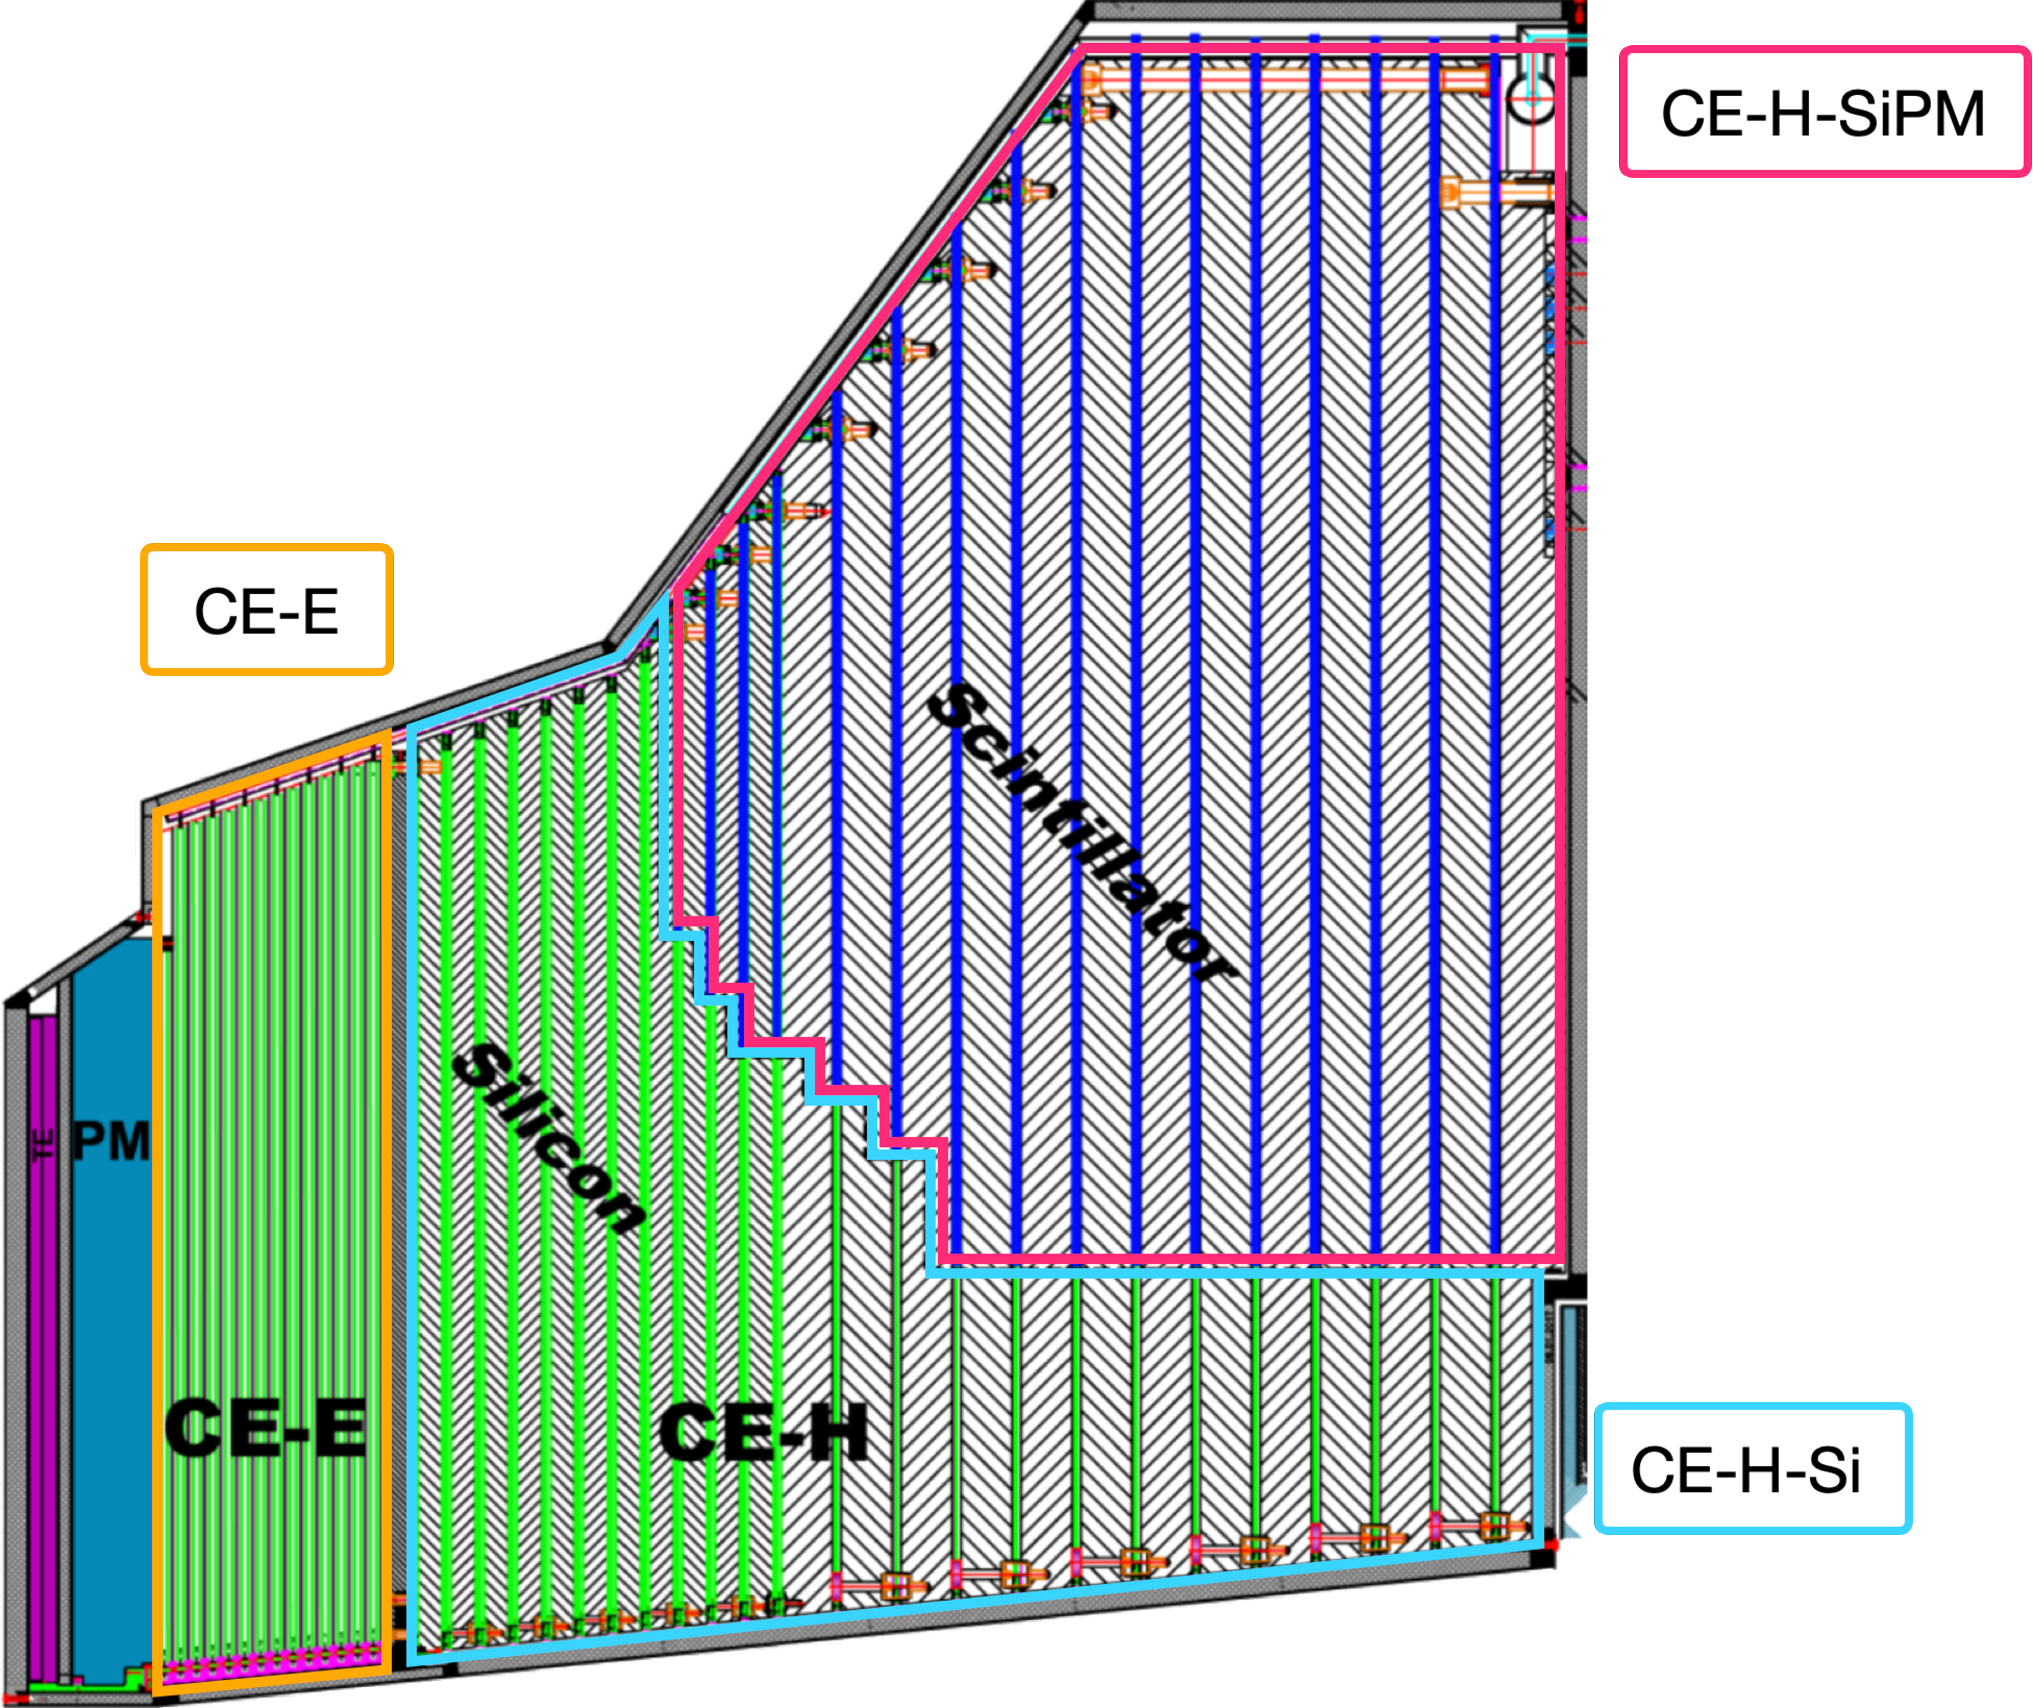
\includegraphics[width=0.6\linewidth]{Figures/HGCAL/HGCALLayers.pdf}
    \caption{Cross section view of the HGCAL. The CE-E and front CE-E compartments comprise silicon-based components. In its latest design, it features 47 layers divided into two regions: 26 silicon-based layers for the Electromagnetic Compartment (CE-E), 21 layers for the Hadronic Compartment (CE-H) using silicon (CE-H-Si) and scintillator-based (CE-H-SiPM) active material. The expected coverage of the HGCAL will range from $|\eta|=1.5$ up to $|\eta|=3.0$.}
    \label{fig:HGCALLayers}
\end{figure}

A longitudinal cross section of the HGCAL is shown in Fig.\ref{fig:HGCALLayers}, where the multiple layers if the Electromagnetic and Hadronic Compartments are visible, along with the different active material used in the two regions.

\bigbreak

In order to cover the area in the most cost-effective manner, the hexagonal geometry for the silicon sensors will be exploited. To reduce the number of modules, the baseline of the sensor size has been adjusted from the initially foreseen 6\mbox{''} design to 8\mbox{''}. An active thickness of 120, 200, or 300 $\mu$m is expected, depending on the detector region.
Each module will comprise several single read-out diodes, hereafter referred to as \textit{cells}, with a 0.5 or 1.0~$\textnormal{cm}^2$ active area, for a total of about six million cells to read out individually in the ultimate detector operation. 
The design, production, and validation of these hexagonal sensors, hereafter referred to as \textit{modules}, is one of the most challenging aspects of the HGCAL project. A more detailed discussion about silicon as active material and the structure of the HGCAL modules is given in Sec.~\ref{sec:Silicon Modules}. 

In the CE-E, the silicon modules will be used to create self-supporting sandwich structures which are commonly referred to as \textit{cassettes}. For this, the modules will be installed on both sides of a copper cooling plate and will be closed with lead plates.

In the low radiation CE-H-SiPM compartment, the scintillating material coupled to SiPMs read-out will be transversely segmented in square shapes with the size of 4 to 30~$\textnormal{cm}^2$, depending on the pseudorapidity position. 
The scintillator modules will be composed of tileboard printed circuit boards (PCBs) with different sizes and shapes. Each tileboard will host from 48 to 96 scintillator tiles individually wrapped into a reflecting layer and characterised by a cavity to contain the SiPM. Each detector on the board will be equipped with an ultraviolet LED next for the calibration and monitoring of the SiPM gain. 

This geometrical configuration amounts to a total active area of 620~$\textnormal{m}^2$ and 370~$\textnormal{m}^2$ for the CE-E and CE-H compartments respectively and provides a compact and cost-effective way to build the entire calorimeter at a reasonable cost while meeting the strict radiation requirements in the high pseudorapidity region.

\begin{figure}
    \centering
    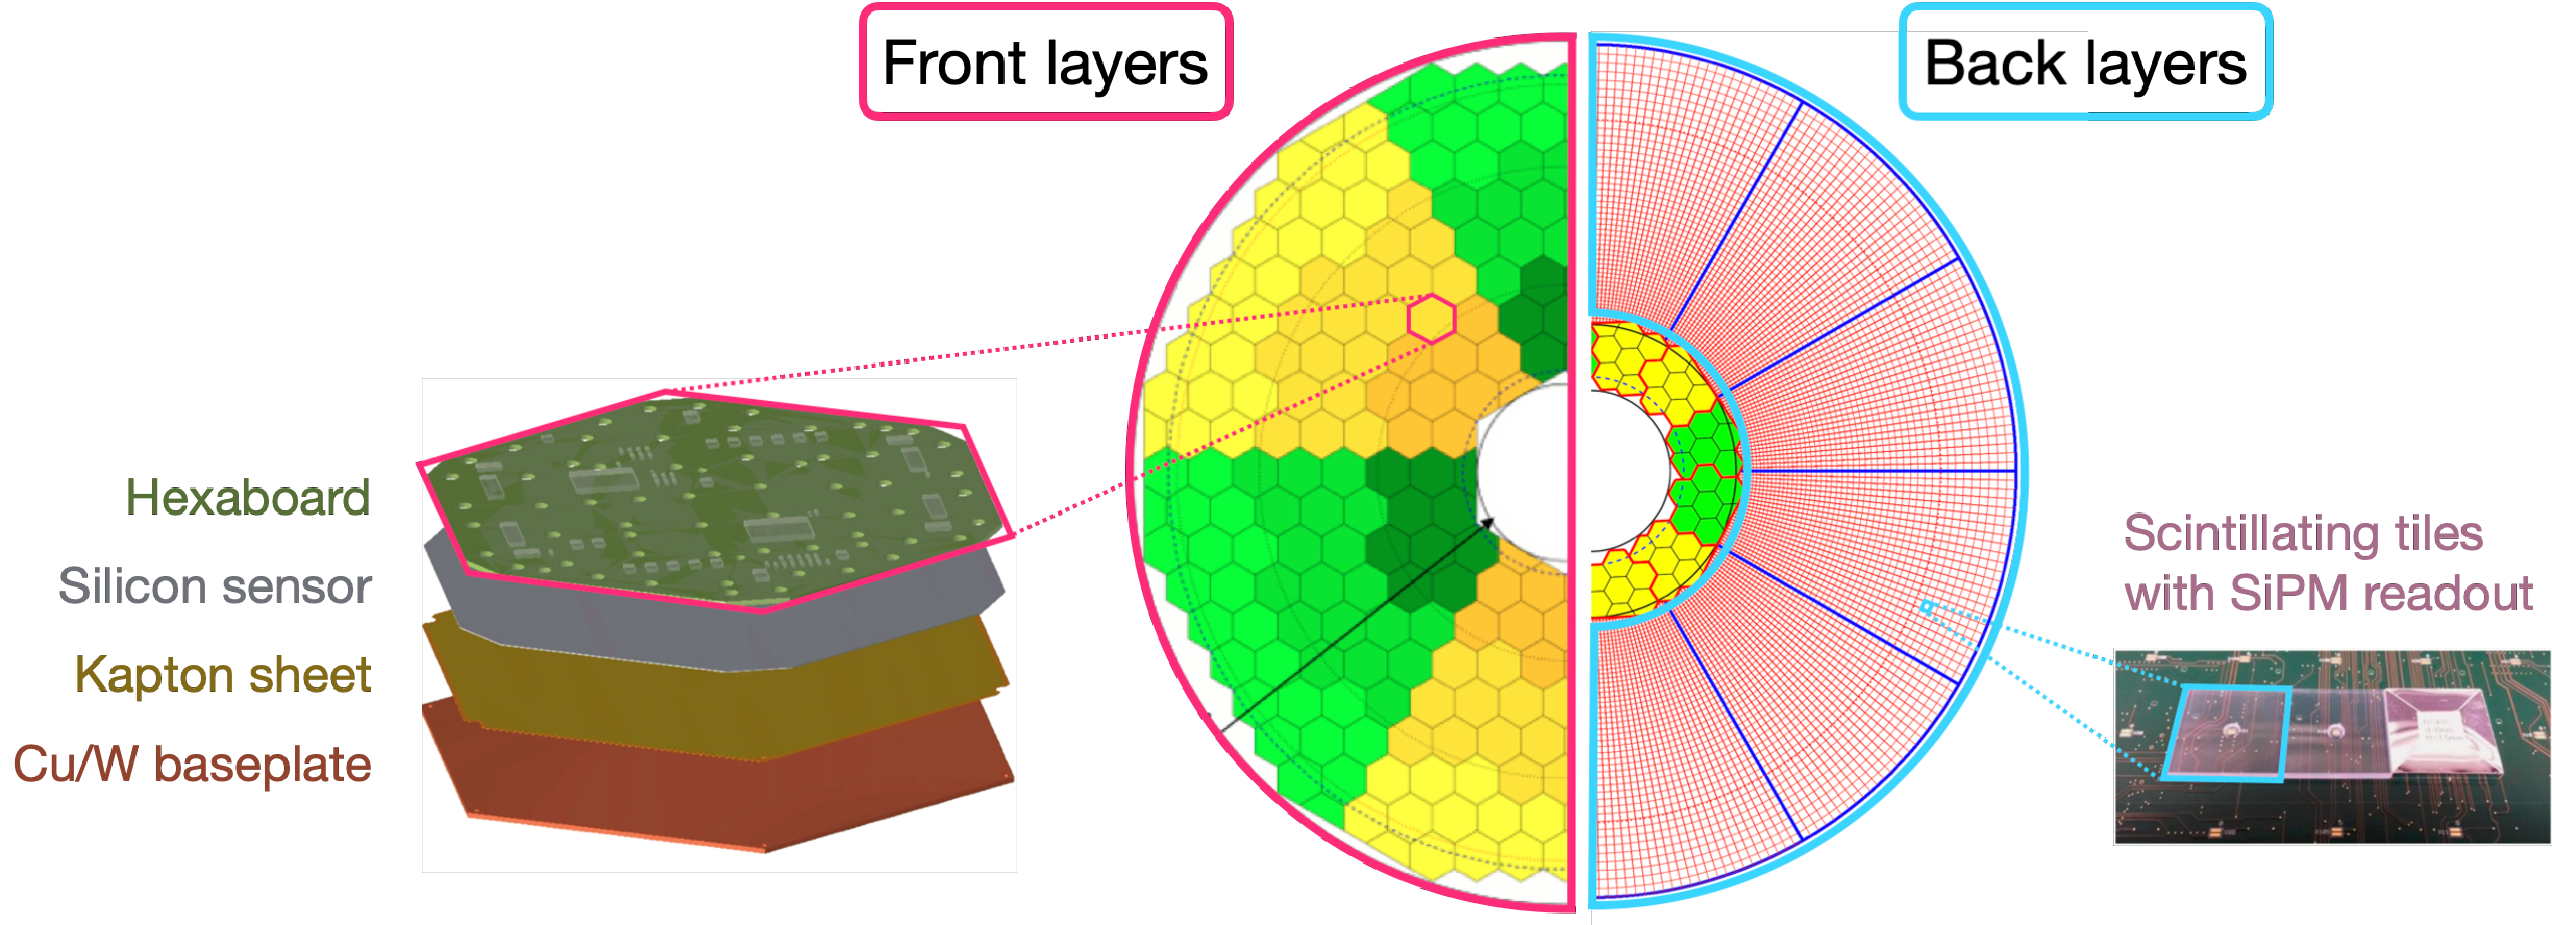
\includegraphics[width=0.9\linewidth]{Figures/HGCAL/FrontBackLayers.pdf}
    \caption{Schematic view of the arrangement of the hexagonal silicon modules in the front layers composing the CE-E and CE-H-Si (left) and of the scintillator tiles employed in the low radiation back layers of the CE-H-SiPM (right).}
    \label{fig:FrontBackLayers}
\end{figure}

The arrangement of the silicon modules in the CE-E and CE-H-Si (front layers) is represented in the left part of Fig.~\ref{fig:FrontBackLayers}, while the right part shows the scintillator tiles employed in the CE-H-SiPM region (back layers).

\bigbreak

The HGCAL design guarantees coverage in the pseudorapidity range $1.5 < |\eta| < 3.0$, featuring both highly granular lateral and longitudinal segmentation. 
The enhanced lateral granularity, combined with the dense absorbers, yields effective individual shower discrimination within the detector. Moreover, the finely segmented longitudinal structure enhances PU rejection, particle identification, and energy resolution. Because of these features, the HGCAL is often referred to as an \textit{imaging}, or 5D, calorimeter, the five dimensions corresponding to the three-dimensional spatial information provided by the fine voxels, the energy deposit in each active material segments, and the timing information with an expected resolution of $\mathcal{O}$(10 ps).

The calibration of the detector will be performed with minimum ionizing particles (MIP). To maintain a reasonable detection of MIPs over the detector's lifetime and ensure a signal-to-noise ratio above one, the effects of radiation damage must be minimized. To achieve this, the HGCAL will have to be operated at a constant temperature of -30~$^{\circ}$C or lower, obtained through a dedicated $\textnormal{CO}_2$ cooling system directly implemented in the copper base plate. 

\subsection{Silicon Modules}
\label{sec:Silicon Modules}

The choice of silicon as the active material in the HGCAL modules is driven by the stringent constraints imposed by the expected physics performance and operating conditions of the detector. 
Silicon sensors ensure the detection of minimum ionizing particles (MIPs) and facilitate precise measurement of high-energey showers, both crucial for the HGCAL's operation efficiency. The former is essential for \textit{in situ} calibrations of the detector, while the latter can be ensured only with a full containment of the showers, which relies on the detector compactness achieved through thin silicon modules and a proper mixture of absorbers.

These requirements are met by silicon sensors, which offer rapid signal response $\mathcal{O}$(10 ns) necessary to keep up with the expected 40 MHz rates at the HL-LHC. Additionally, silicon module production benefits from established large-scaled industrial capabilities, allowing for relatively short lead times.

The validation of the silicon modules structure has been cornerstone of the project since the approval of the HGCAL Technical Proposal (TP) in 2015. Several proof-of-concept modules, produced by Hamamatsu Photonics K.K. (HPK), have undergone extensive testing in beam experiments between 2016 and 2017. Insights from these tests, incorporated into the 2018 HGCAL Technical Design Report (TDR), form the foundation for understanding the properties of silicon modules crucial for such a complex detector.

\bigbreak

The HGCAL will require approximately $27\,000$ silicon detector modules to be assembled and installed in its electromagnetic (CE-E) section and part of the hadronic (CE-H) section.

Each module consists of stacked layers comprising the printed circuit board (PCB), labeled \textit{hexaboard}, where the front-end electronics are installed, a silicon sensor, and a gold-plated Kapton sheet providing HV connection to the sensor back-plane and electrical insulation. The baseplate, made of materials such as CuW or Cu, provides enough rigidity to support the module whilst minimizing the total radiation length and dissipating the heat through a dedicated cooling system.

The silicon modules will be further segmented into either 192, for low-density (LD), or 432 individual diodes, for high-density (HD) modules. The diodes will act as sensor cells and have a separate read-out channel.

\begin{figure}
    \centering
    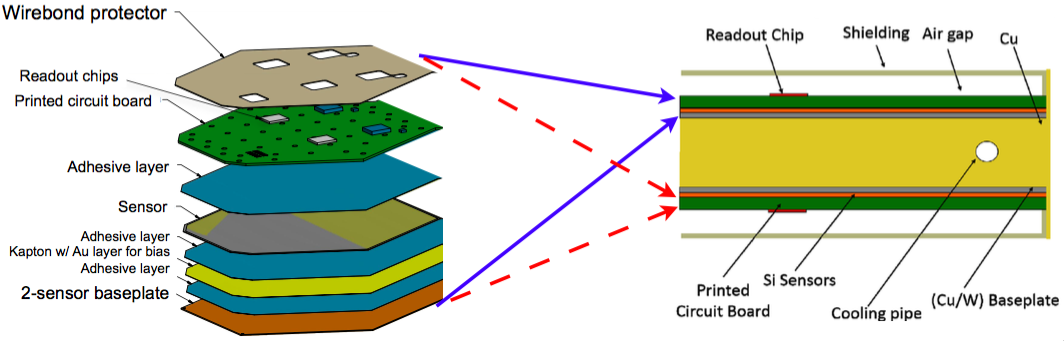
\includegraphics[width=0.9\linewidth]{Figures/HGCAL/ModuleDesign.png}
    \caption{Composition of a silicon module and placement in the copper plate. Each module is a stack of different layers, starting with a baseplate at the bottom, covered with a gold plated Kapton foil on which stands the silicon sensor. A protected PCB with read-out chip is placed on top.}
    \label{fig:ModuleDesign}
\end{figure}

A schematic view of the structure of a typical HGCAL module is given in Fig.~\ref{fig:ModuleDesign}.

\subsection{Plastic Scintillation Tiles}
\label{sec:Plastic Scintillation Tiles}

The remaining portion of the CE-H compartment will incorporate scintillator as the active material in regions where the integrated dose remains low-enough ($<3$~kGy) to maintain optimal performance throughout the entire lifespan of the HL-LHC. 
This approach will also ensure effective muon identification in the $\eta>2.4$ region, where muon chambers are not available.

The scintillator will be crafted into small squared tiles, with the scintillation light reflected by a wrapping foil and directly read-out by a SiPM optically coupled through a small \textit{dimple} in the centre of one face of each tile. The SiPMs will be mounted on printed circuit boards, matched to the appropriate tiles. 
The system is illustrated in Fig.\ref{fig:ScintillatorTiles}.

In conformity with the CMS endcap's geometry, the scintillator cells will be arranged in an $r,\phi$ grid. As a result, cells closer to the beam line will be significantly smaller (4~$\textnormal{cm}^2$) than those at the outer edge (32~$\textnormal{cm}^2$). 

The area instrumented with scintillator will be subdivided into tile-modules consisting of a tileboard and the scintillator tiles. These tile-modules will then be connected together to form a 10~$^{\circ}$ detector unit. Six such units will be placed next to each other and combined with silicon modules into cassettes, covering 60~$^{\circ}$ each. Finally, six cassettes will collectively complete the calorimeter layer around the beam pipe.

\begin{figure}
    \centering
    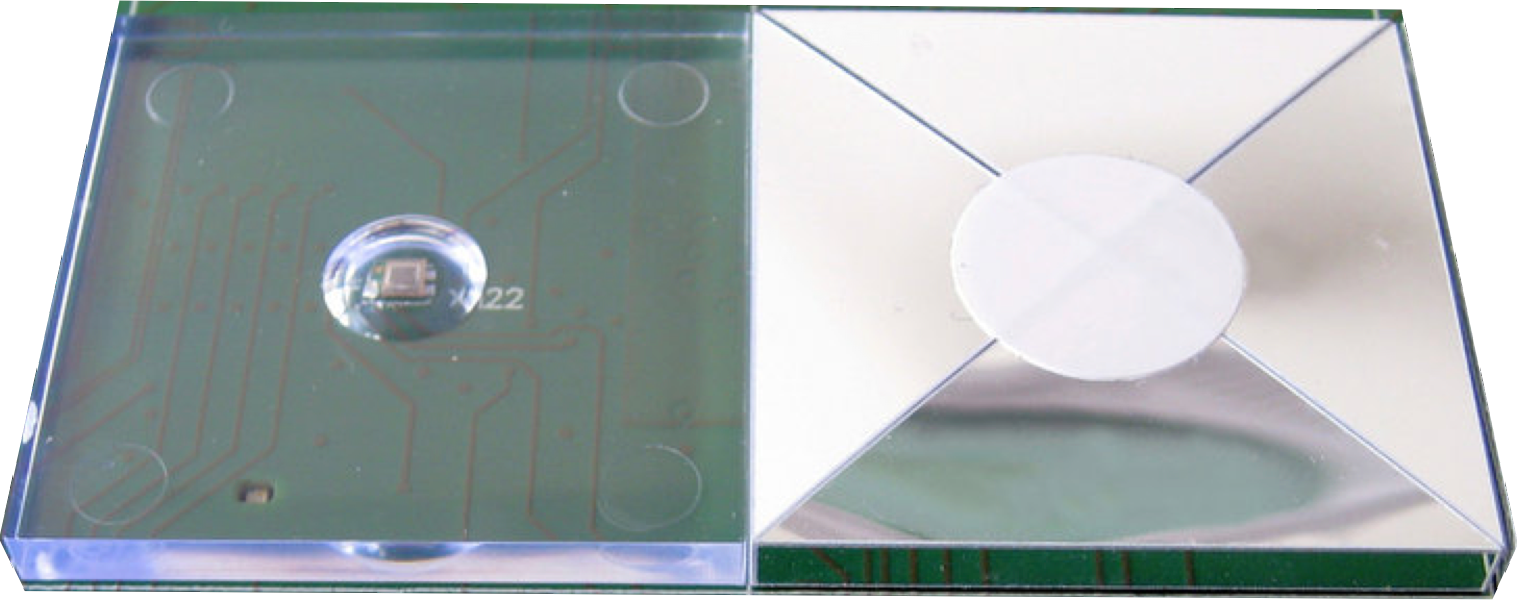
\includegraphics[width=0.5\linewidth]{Figures/HGCAL/ScintillatorTiles.pdf}
    \caption{Example of two $3\times3\textnormal{cm}^2$ scintillator tiles with a central dimple, unwrapped (left) and wrapped (right), mounted on a PCB housing one SiPM per tile, used as a prototype for the HGCAL project.}
    \label{fig:ScintillatorTiles}
\end{figure}

%%%%%%%%%%%%%%%%%%%%%%%%%%%%%%%%%%%%%%%%%%%%%%%%%%%%%%%%%%%%%%%%%%%%%%%%%%%%%%%%%%%%%%%%%%%%
%%%%%%%%%%%%%%%%%%%%%%%%%%%%%%%%%%%%%%%%%%%%%%%%%%%%%%%%%%%%%%%%%%%%%%%%%%%%%%%%%%%%%%%%%%%%
%%%%%%%%%%%%%%%%%%%%%%%%%%%%%%%%%%%%%%%%%%%%%%%%%%%%%%%%%%%%%%%%%%%%%%%%%%%%%%%%%%%%%%%%%%%%
%%%%%%%%%%%%%%%%%%%%%%%%%%%%%%%%%%%%%%%%%%%%%%%%%%%%%%%%%%%%%%%%%%%%%%%%%%%%%%%%%%%%%%%%%%%%

\section{The HGCAL Front-End Electronics}
\label{sec:The HGCAL Front-End Electronics}

One of the most challenging aspects in the design of the HGCAL silicon and scintillator modules is the front-end (FE) electronics. 

The FE electronics is responsible for several critical functions within the HGCAL system. It measures and digitizes the charge deposited in the silicon sensor pads or generated in the SiPMs, providing precise time measurements for the pulses. It transmits the digitized data to the back-end (BE) electronics located in the service cavern. It also computes, at each bunch crossing, the digital sums of neighboring cells, tailored to the specific cell sizes ($2\times2$ cells for 1~$\textnormal{cm}^2$ pads silicon sensors, 3 cells for 0.5~$\textnormal{cm}^2$ sensors, and 2 cells for scintillator tiles) to be transmitted to the trigger BE electronics to build trigger primitives.

Besides the unprecedented readout segmentation, the performance requirements for the FE electronics are extremely stringent, particularly for the silicon part of the detector:
\begin{itemize}
    \item [-] Low noise and large dynamic range, spanning from approximately 0.2~fC to 10~pC, equivalent to 16 bits. This range enables the detection of MIPs in the silicon sensors and the recording of high-energy deposits from electromagnetic showers. 
    The electronics noise must be below 2000 electrons for a 65~pF capacitance pad to allow MIP visibility during the whole operation.
    \item [-] Integral linearity must exceed 1$\%$ across the entire dynamic range.
    \item [-] Timing information with a precision better than 100~ps for pulses above 12~fC, corresponding to about 3~MIPs in the 300~$\mu$m silicon sensors.
    \item [-] Fast shaping time (peaking-time $<20$~ns) to minimize the out-of-time pileup: the pulse should be dropped to less than 20$\%$ by the next bunch crossing.
    \item [-] On-detector digitization and data processing for zero suppression, linearization and summing of the trigger data.
    \item [-] Maximum latency of 36~bunch crossings for the trigger primitives at the output of the detector.
    \item [-] Buffering of the data to accommodate the 12.5~$\mu$ms latency of the L1 trigger.
    \item [-] High-speed read-out links to interface with the 10~Gb/s low-power GBT (LpGBT) serializer.
    \item [-] Low power budget ($<20$~mW per channel), typically limited by cooling power.
\end{itemize}

Following the LHC data-taking conditions, the acquisition chain must handle consecutive event arrivals at 40~MHz without data erasure.
Moreover, the FE electronics will face a harsh radiation environment which will reach 200~Mrad at the end of life and requires extremely high radiation tolerance.

\begin{figure}
    \centering
    \includegraphics[width=0.95\linewidth]{Figures/HGCAL/Hexaboards.pdf}
    \caption{Plan view of two hexaboards housing 6 High Density (HD) HGCROC read-out chips: each chip is connected to 72 hexagonal cells. The connector will be used for the assembly of the motherboard, containing the ECON-D and ECON-T concentrator chips.}
    \label{fig:Hexaboards}
\end{figure}

\bigbreak

The very first step of the FE electronics read-out chain is the HGCal Read-Out Chip (HGCROC), which measures at 40~MHz frequency the charge and the time of arrival of each particle crossing the HGCAL cells. The HGCROC is directly bonded through a ball-grid array to the hexaboard and has multiple channels connected to individual cells. 
The read-out chips, the linear voltage regulators (LVR), and any other passive and service components are mounted on a hexagonal module PCB, called \textit{hexaboard}, which is glued onto the silicon sensor. Imprinted on the hexaboard are also the pads for connections to the next board in the chain, labeled \textit{motherboard}. These connections also supply the LV, receive and transmit signals and data. 

\bigbreak

The next level of the FE electronics includes the concentrators, located on the motherboards sitting 1.6~mm above the hexaboards. Each motherboard serves from one to six modules, depending on the occupancy of the sensors. The surfaces including the components of the hexaboard and of the motherboard face each other in order to reduce the overall thickness. 

The architecture of the very FE electronics chain on the hexaboards is summarised in Figure~\ref{fig:Hexaboards}. 

%%%%%%%%%%%%%%%%%%%%%%%%%%%%%%%%%%%%%%%%%%%%%%%%%%%%%%%%%%%%%%%%%%%%%%%%%%%%%%%%%%%%%%%%%%%%
%%%%%%%%%%%%%%%%%%%%%%%%%%%%%%%%%%%%%%%%%%%%%%%%%%%%%%%%%%%%%%%%%%%%%%%%%%%%%%%%%%%%%%%%%%%%
%%%%%%%%%%%%%%%%%%%%%%%%%%%%%%%%%%%%%%%%%%%%%%%%%%%%%%%%%%%%%%%%%%%%%%%%%%%%%%%%%%%%%%%%%%%%
%%%%%%%%%%%%%%%%%%%%%%%%%%%%%%%%%%%%%%%%%%%%%%%%%%%%%%%%%%%%%%%%%%%%%%%%%%%%%%%%%%%%%%%%%%%%

\section{The HGCROC3 architecture}
\label{sec:The HGCROC3 architecture}

With an extraordinary technical effort to meet all the FE electronics requirements, the HGCROC3 is the final version of the ASIC specifically designed by the CMS Collaboration, in collaboration with the Omega Microelectronics Center at École Polytechnique, to read-out the modules of the future HGCAL. 
Two versions of the same read-out architecture have been developed, for the silicon (Si) and the scintillator tiles (SiPM) sections, where the latter is obtained by only adding a current conveyor and adapting the preamplifier of the silicon variant.

\bigbreak

The main function of the HGCROC3 is to measure and digitize the charge deposit and provide high precision time information of the particles crossing the detector layers. It is also able to compute the energy sum of neighbouring cells in order to contribute to the Level-1 (L1) trigger decision. 
The chip features 78 channels, each consuming less than 15 mW power, and is designed in a radiation-hardened 130~nm CMOS technology. Among the channels, 72 serve as standard cells read-out, 2 function as calibration cells read-out, and the remaining 4 channels are not connected to any sensor cells, serving for common-mode noise estimation. 

The layout is symmetrically divided into two parts, or \textit{halves}, as shown in Figure~\ref{fig:TowHalves}.
In Figure~\ref{fig:Architecture} a schematics of the inner architecture of the ASIC is presented: the structure and characteristics of each component are described in the following paragraphs.

\begin{figure}
    \centering
    \includegraphics[width=0.75\linewidth]{Figures/HGCAL/TwoHalves.pdf}
    \caption{Layout of the HGCROC3 ASIC: the chip is divided into two symmetrical parts. The voltage reference is positioned near the chip's edge, the ADC reference and TDC controls are located in the central region.}
    \label{fig:TowHalves}
\end{figure}

\paragraph{Data path}
The data path is the core of the chip, replicated for 72 channels of the full analog chain, 4 common mode channels for the coherent noise subtraction, and 2 calibration channels for the MIP calibration. This component extracts from the signal input charge three digitised quantities to be sent to the back-end electronics: the ADC for the charge measurement, the ToA (Time-of-Arrival) for the time measurement, and the ToT (Time-over-Threshold) for the charge measurement of saturated signals. 

The charge digitization is achieved by a 10-bit~ADC in the linear range of the preamplifier; when it saturates, a 12-bit Time-to-Digital Converter (TDC) with 50~ps binning over 200~ns range provides the charge information by measuring the ToT. The ToA digitization is carried out by a similar dedicated 10-bit TDC with 25~ps binning over 25~ns range.
The low-noise preamplifier gain can be adapted to different detector regions, where the MIP energy deposit can vary depending on the sensor thickness and irradiation condition.
Under HL-LHC conditions, certain regions of the detector may exhibit notably high occupancy rates, reaching up to 50$\%$ of fired cells per bunch crossing: it is thus important that the analog shaper drops the signal sample to less than 20$\%$ by the next bunch crossing to mitigate the out-of-time pile-up.

Beyond the analog performance, the chip embeds a large part of digital processing to manage the Data and the Trigger paths. A 512-depth DRAM (RAM1) is used as a circular memory to buffer the data to accommodate the 12.5~$\mu$s latency of the L1 trigger, and a 32-depth DRAM (RAM2) is used as a FIFO after the L1 selection.
Two 1.28~Gbps links are dedicated to send out the full event information of the selected bunch crossings after a L1 request.

\begin{figure}
    \centering
    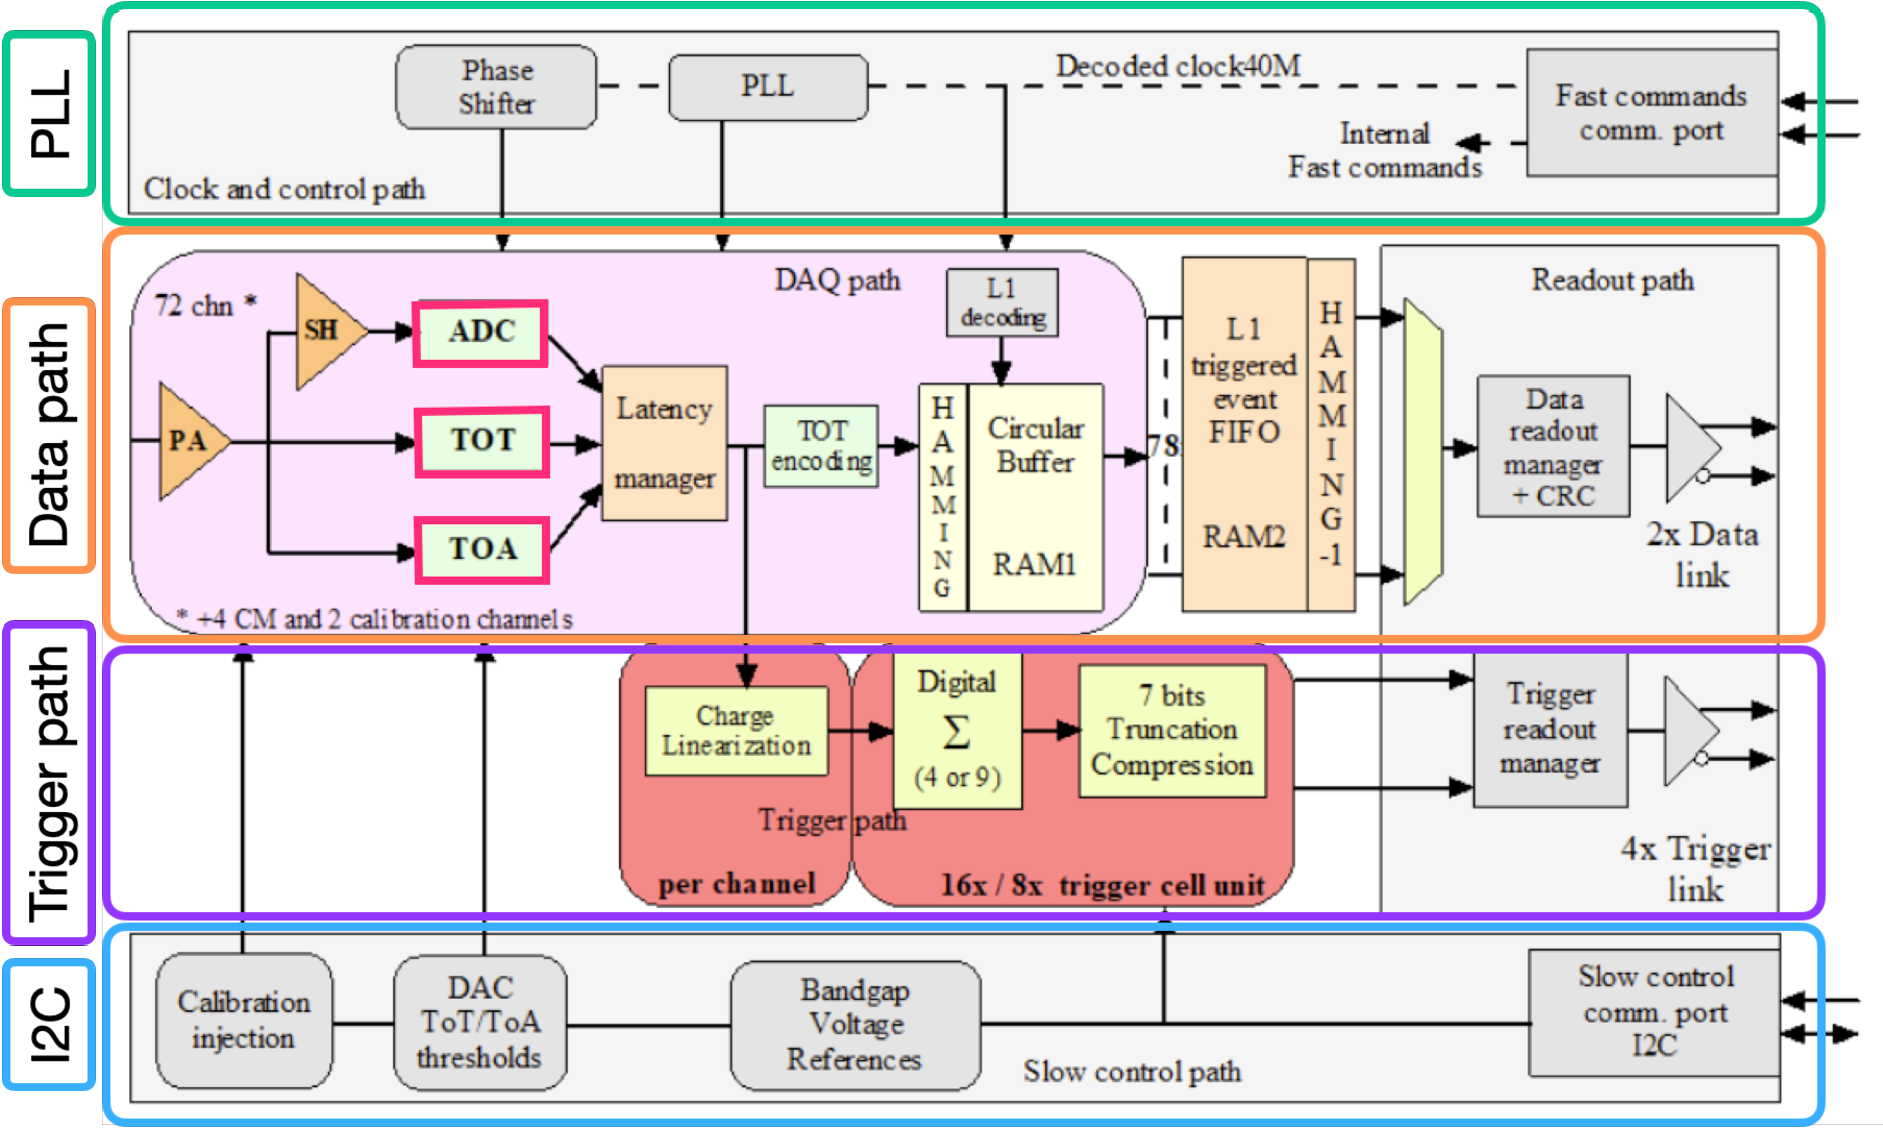
\includegraphics[width=0.75\linewidth]{Figures/HGCAL/Architecture.pdf}
    \caption{Architectural overview of the HGCROC3 read-out ASIC. The main parts composing the Data path, Trigger path, PLL and I2C have been highlighted.}
    \label{fig:Architecture}
\end{figure}

\paragraph{Trigger path}
The trigger path computes an image of the deposited charge at each bunch crossing, by summing and compressing data over neighbouring channels. The two charge-related quantities from the channel information (ADC and ToT) are fed into the trigger path. The chip performs the data processing with a charge linearisation over the ADC and ToT range and computes the energy sums over 4 (9) adjacent channels for the LD (HD) modules. After compressing the information to 7 bits, it sends the trigger data to the ECON-T concentrator chip.
Four $1.28\,\textrm{Gbps}$ differential links are devoted to send the energy sums for the L1 trigger decision.

\paragraph{PLL}
The Phase-Locked Loop (PLL) is an analog clock synthesizer receiving the 40~MHz LHC clock and providing all the other clock frequencies - from 160~MHz to 1.28~GHz - used by the circuit.
The main challenge for the PLL circuit is to ensure that all the clocks' phases are aligned to the LHC 40~MHz input clock: a low noise digital Phase Frequency Detector (PFD) continuously checks for possible phase misalignments and, in case one is found, adjusts the voltage-controlled oscillator (VCO) in order to temporarily increase or decrease the frequency and realign the phase. The PLL is an essential component for the HGCROC3 functioning and has been intensively tested during the irradiation campaigns, as described in Sections~\ref{subsec:Total Integrated Dose} and \ref{subsec:Single Event Effect}.

\paragraph{I2C}
The Inter-Integrated Circuit (I2C) is an internal static memory register storing the chip's configuration parameters.
The I2C protocol is used to set or read the more than 7900 parameters, distributed into 8 internal registers.
A Fast Command block is used to read and write the configuration parameters, to configure the operating mode of the system (link synchronisation, reset, calibration, L1 request, etc.), and to communicate with the device.

%%%%%%%%%%%%%%%%%%%%%%%%%%%%%%%%%%%%%%%%%%%%%%%%%%%%%%%%%%%%%%%%%%%%%%%%%%%%%%%%%%%%%%%%%%%%
%%%%%%%%%%%%%%%%%%%%%%%%%%%%%%%%%%%%%%%%%%%%%%%%%%%%%%%%%%%%%%%%%%%%%%%%%%%%%%%%%%%%%%%%%%%%
%%%%%%%%%%%%%%%%%%%%%%%%%%%%%%%%%%%%%%%%%%%%%%%%%%%%%%%%%%%%%%%%%%%%%%%%%%%%%%%%%%%%%%%%%%%%
%%%%%%%%%%%%%%%%%%%%%%%%%%%%%%%%%%%%%%%%%%%%%%%%%%%%%%%%%%%%%%%%%%%%%%%%%%%%%%%%%%%%%%%%%%%%

\section{Characterisation and testing of the HGCROC3}
\label{sec:Characterisation and testing of the HGCROC3}

% When I arrived the new  HGCROC3 had just arrived and we had to test their performance in order to check whether the met the requirements
% What are the differences between HGCROC2 and 3?

The characterisation of the HGCROC3 is a crucial step towards validating the chip design, ensuring expected performance within acceptable limits, and guaranteeing reliability in operations. 
Through meticulous design characterisation and comprehensive testing, it is possible to identify potential issues such as power consumption irregularities, temperature sensitivities, or timing violations, to validate the reliability and robustness of the final product. 
Detecting defects in advance also allows for necessary corrections to be made in the design before final submission and large-scale production.

\bigbreak

\begin{figure}
    \centering
    \includegraphics[width=0.7\linewidth]{Figures/HGCAL/Mezzanine.pdf}
    \caption{Experimental set-up for the characterisation and testing of the HGCROC3. The mezzanine board  supports the testing of a prototype of the HGCROC3. The chip is bonded to a mezzanine, that can be mounted on a PCB (right), which is connected to a FPGA system (left) interfaced with the PC for the data acquisition.}
    \label{fig:Mezzanine}
\end{figure}

The HGCROC3 testing has been performed in the electronics laboratory, using various types of test benches:
\begin{itemize}
    \item \textit{Mezzanine} boards, on which all the power supplies are kept separated and it is possible to check the performance of the circuit in an optimistic environment, where the power supplies couplings are reduced.
    \item \textit{Socket} boards, where multiple chips can be tested in series: two socket versions have been produced, designated for manual or automated operations respectively.
\end{itemize}

Figure~\ref{fig:Mezzanine} shows the experimental set-up for the HGCROC3 testing, using a mezzanine board that can host only one prototype. This configuration is used for testing a small number of prototypes in a optimistic environment. A dedicated PCB designed to support the mezzanine is used to regulate the bias voltage and measure the power consumption in different components of the chip. The communication is controlled by a FPGA system developed at CERN, interfaced with a PC for data acquisition.

This section outlines the main procedures for calibrating and testing the HGCROC3, which are essential to comprehend and evaluate its performance; it illustrates the expected response of the chip to injected charge in terms of ADC, ToA and ToT measurement; finally, it presents the results from a preliminary batch testing on approximately 200 HGCROC3 prototypes and describes the unexpected behaviour caused by design defects that have been addressed in new submission of the chip design, the HGCROC3b.

\subsection{The calibration procedure}
\label{subsec:The calibration procedure}

The HGCROC3 needs to be adaptable to a wide range of scenarios, in order to ensure consistent performance across the numerous modules and channels. The presence of potential discrepancies resulting from the chip manufacturer and the selected technology might cause fluctuations between different chips or channels belonging to the same device. As a consequence, the chip design integrates configurable parameters aimed at addressing various aspects, from the optimisation of the DC levels to the mitigation of radiation-induced damage. 

A calibration procedure is essential to find the optimal parameters and constitutes the very first operation to be performed before testing the chip. It includes the optimisation of the pedestal value for each channel, the ToA and ToT thresholds setting, and the definition of the correct phase for the signal sampling. A summary of the methodologies for the chip calibration is described in the following paragraphs.

\subsubsection{The pedestal calibration}
\label{subsubsec:The pedestal calibration}

\begin{figure}
    \centering
    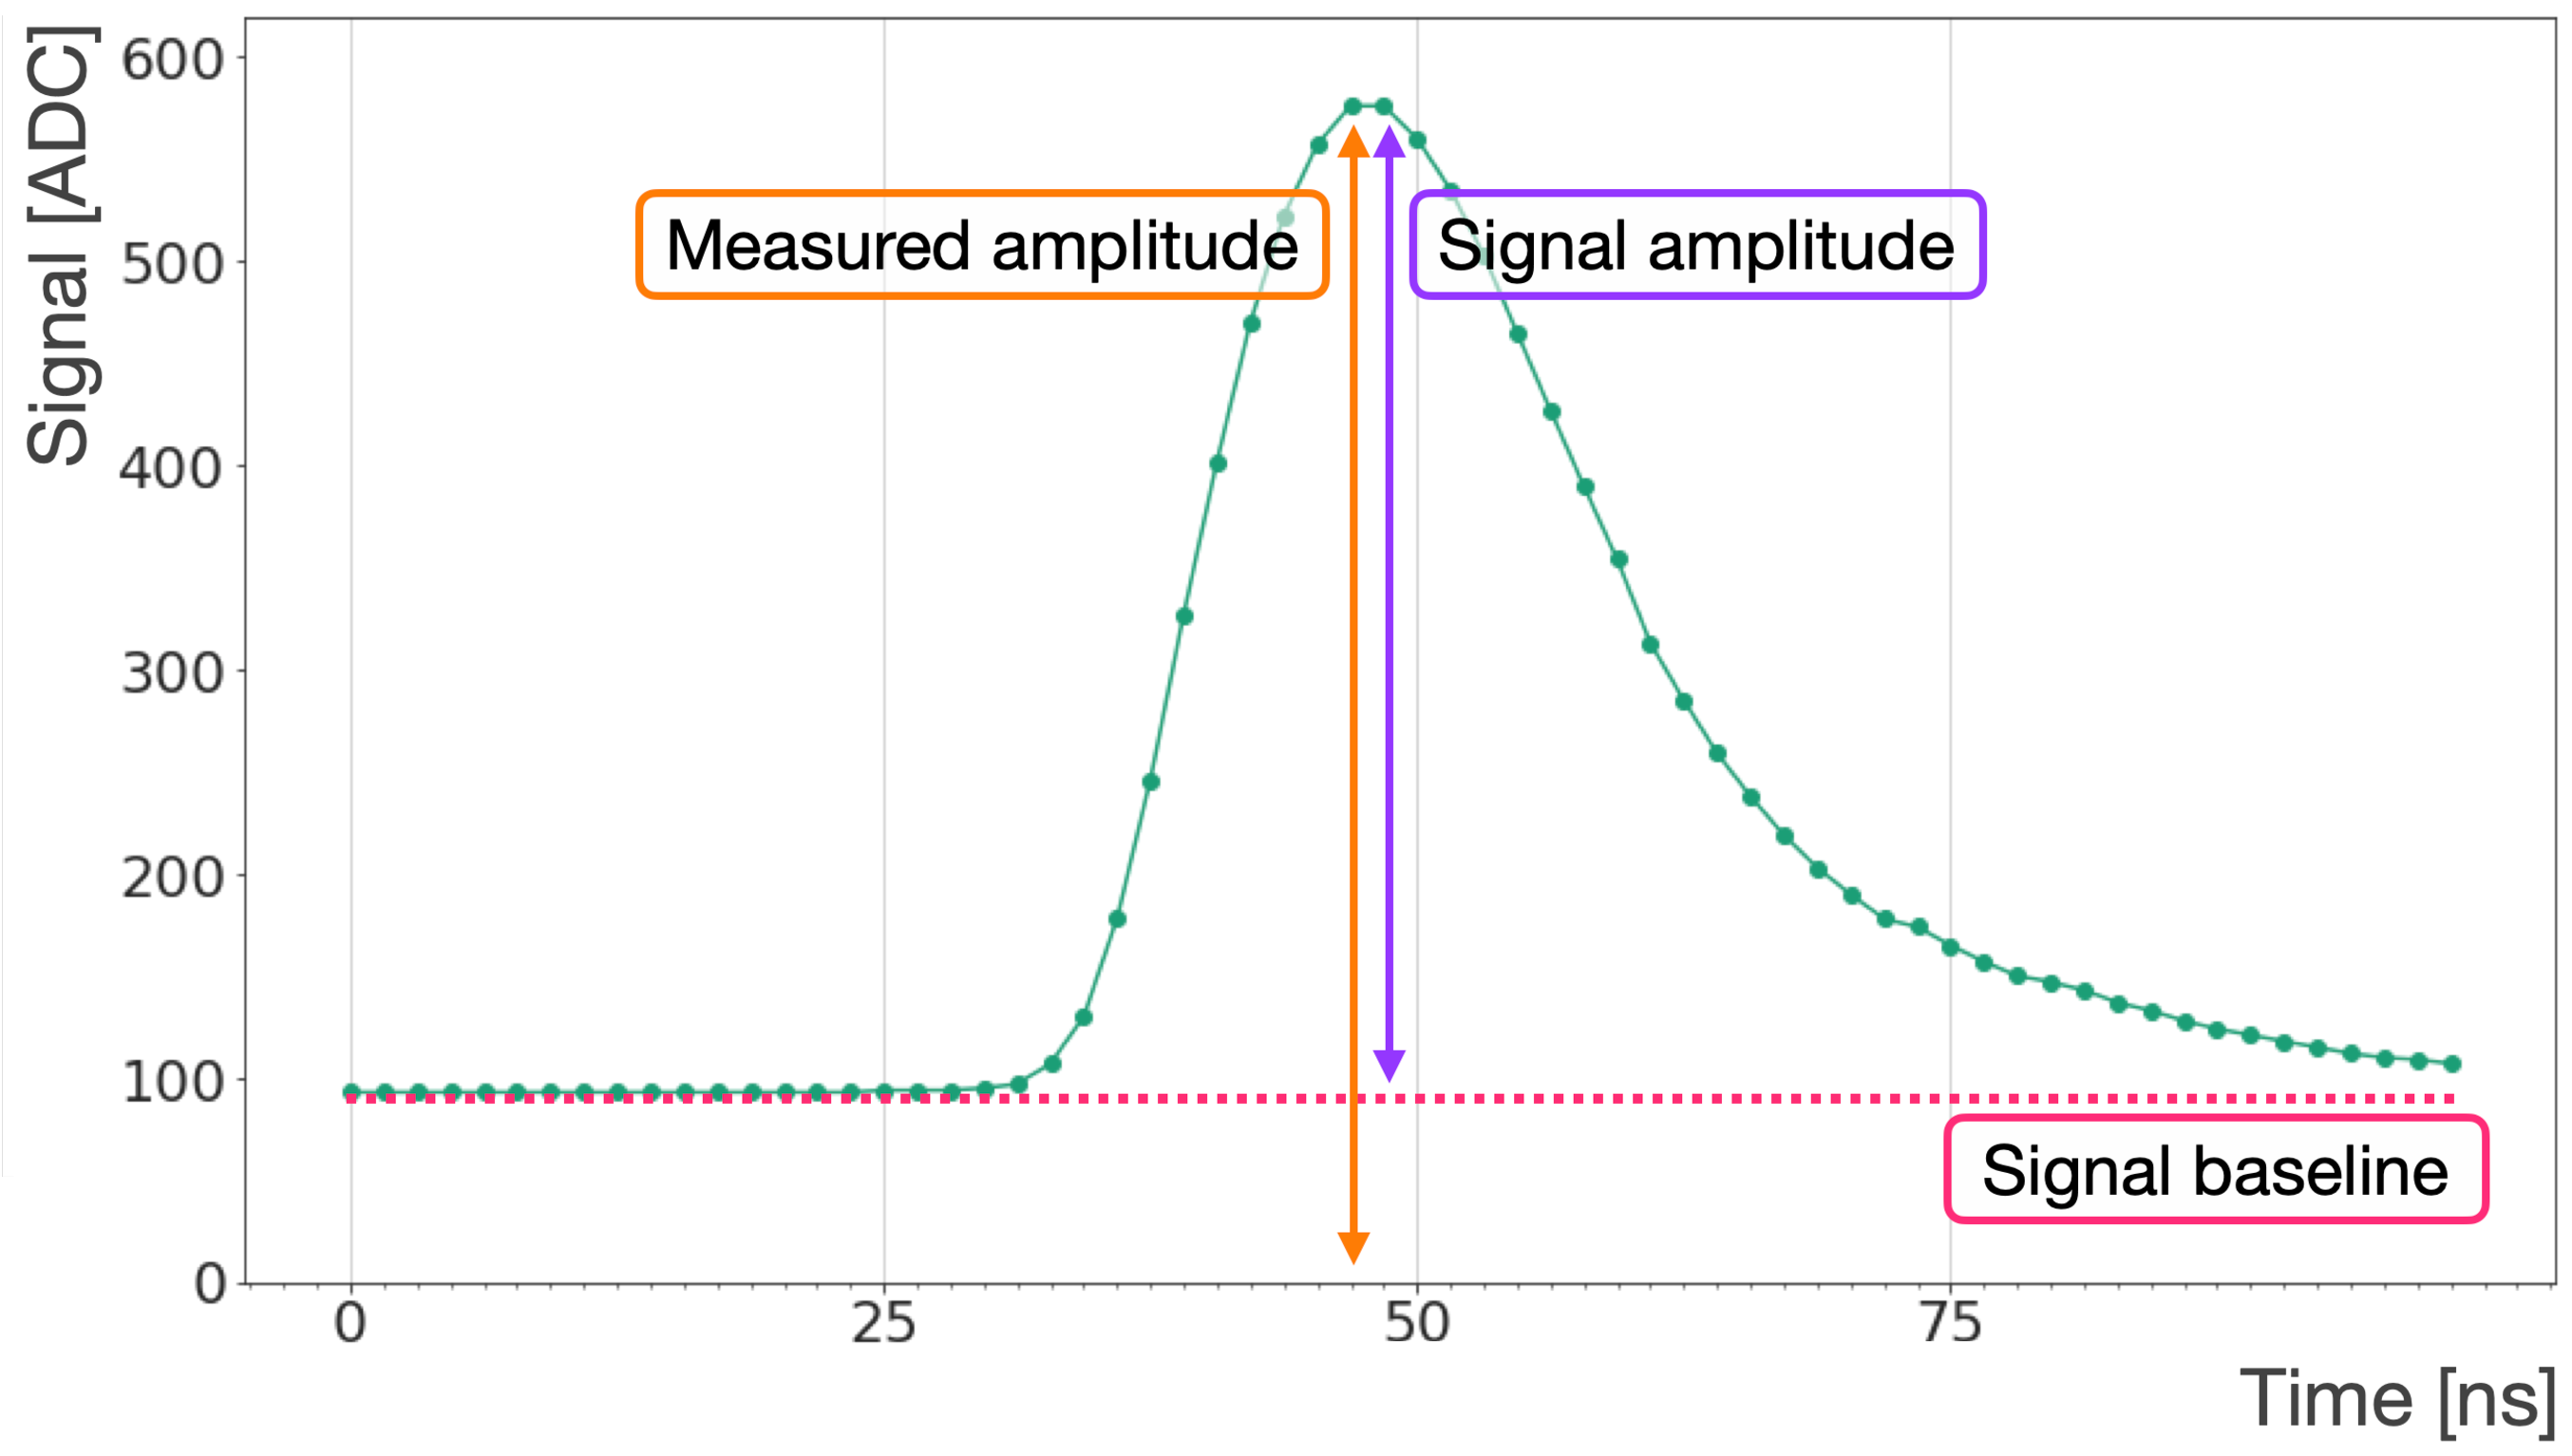
\includegraphics[width=0.6\linewidth]{Figures/HGCAL/SignalBaseline.pdf}
    \caption{A typical signal shape recorder by the HGCROC3: the pink line shows the pedestal baseline. The picture highlights the difference between the measured amplitude (orange) and the real signal amplitude (purple).}
    \label{fig:SignalBaseline}
\end{figure}

The initial step of the chip calibration procedure consists in the tuning of the pedestal values. The pedestal is the baseline of the signal, i.e. the ADC recorded value when no input is present. On the one hand, the pedestal value should be minimised, in order to fully exploit the dynamic range for the measurement of the signal amplitude. On the other hand, having a non-zero pedestal is a common practice in electronics devices in order to avoid a possible change in the signal polarisation due to electronic noise or to fluctuations of the ground potential.
Figure~\ref{fig:SignalBaseline} shows a typical signal shape recorded by the HGCROC3 with a pedestal value around 100~ADC counts. Since every signal is built on top of the baseline, it is important to know the pedestal value and subtract it from the measured amplitude in order to extract the real signal amplitude.

\bigbreak

Before the calibration procedure, the 78 independent channels of the HGCROC3 present a large dispersion in their pedestal values, as shown in the left plot of Figure~\ref{fig:Pedestal}. 
A channel-wise parameter (\texttt{Trim\_Inv}) is available in the I2C register to change the pedestal of each channel independently: the parameter is coded into 6 bits, corresponding to 64 possible values.
The \textit{local} per-channel pedestal trimming is performed by scanning all possible values of the parameter and defining as a target the maximum, between all the pedestal values, for a \texttt{Trim\_Inv} value of 0. The \texttt{Trim\_Inv} of each channel will be set to the value giving a pedestal as close as possible to the target.
The full scan of the pedestal trimming value is performed separately for each half of the HGCROC3 and is shown in Figure~\ref{fig:PedestalScan}.

\begin{figure}
    \centering
    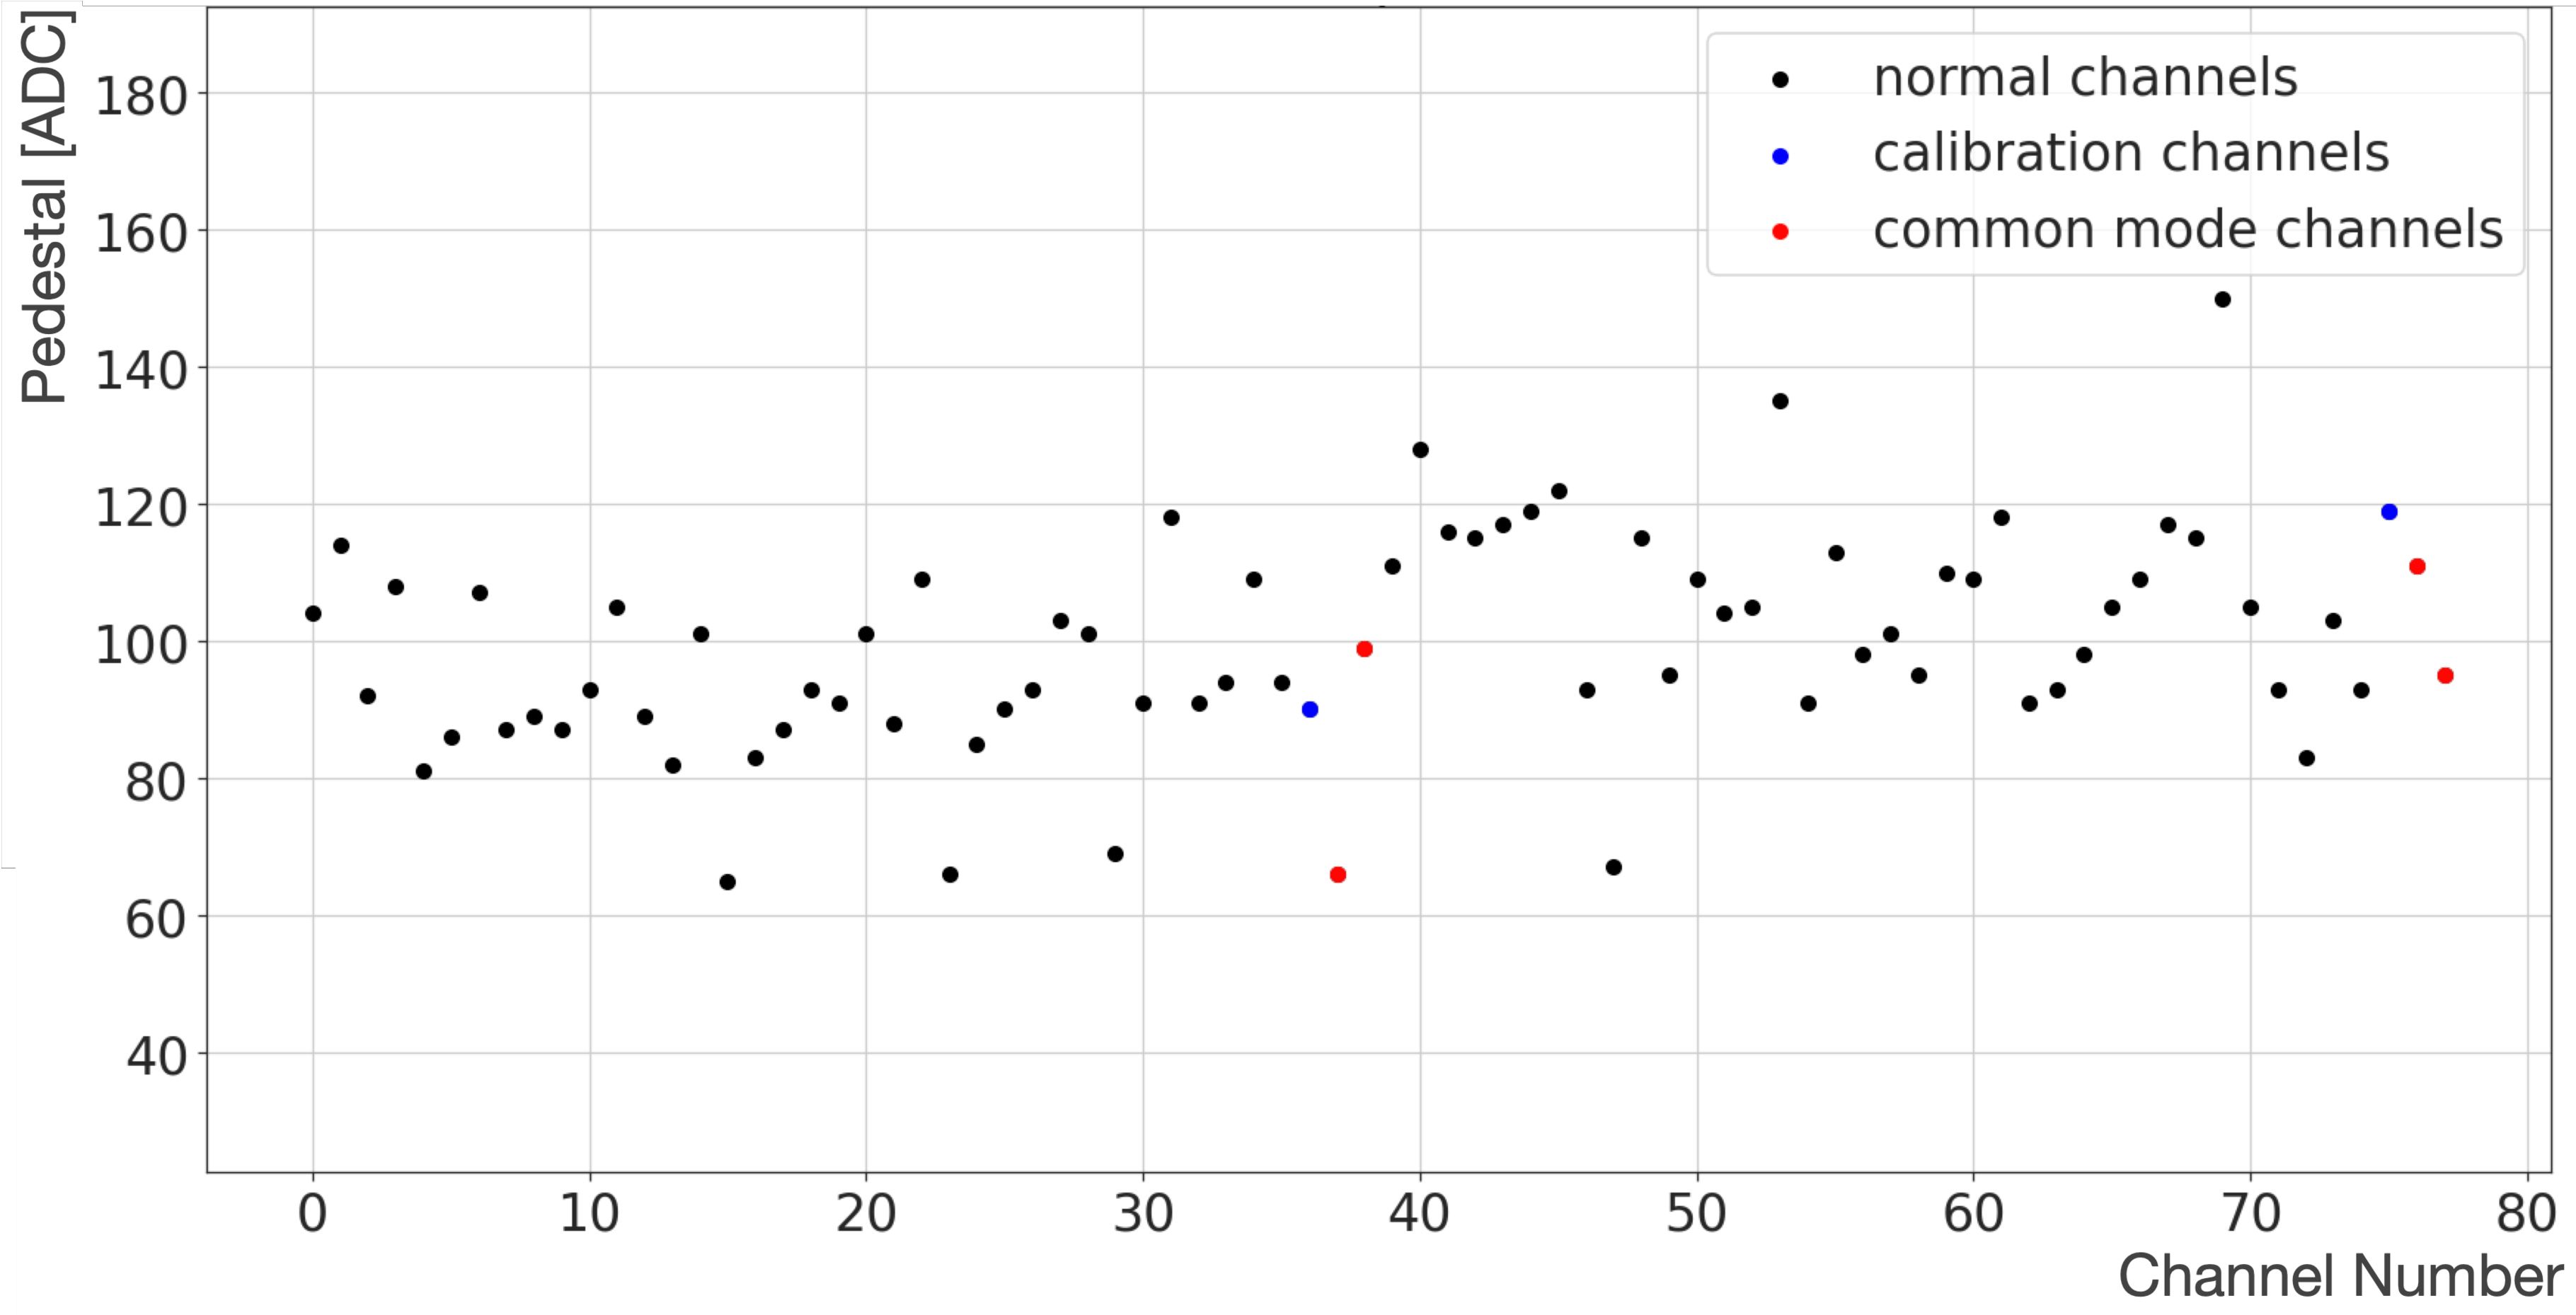
\includegraphics[width=0.49\linewidth]{Figures/HGCAL/Pedestal_0.pdf}
    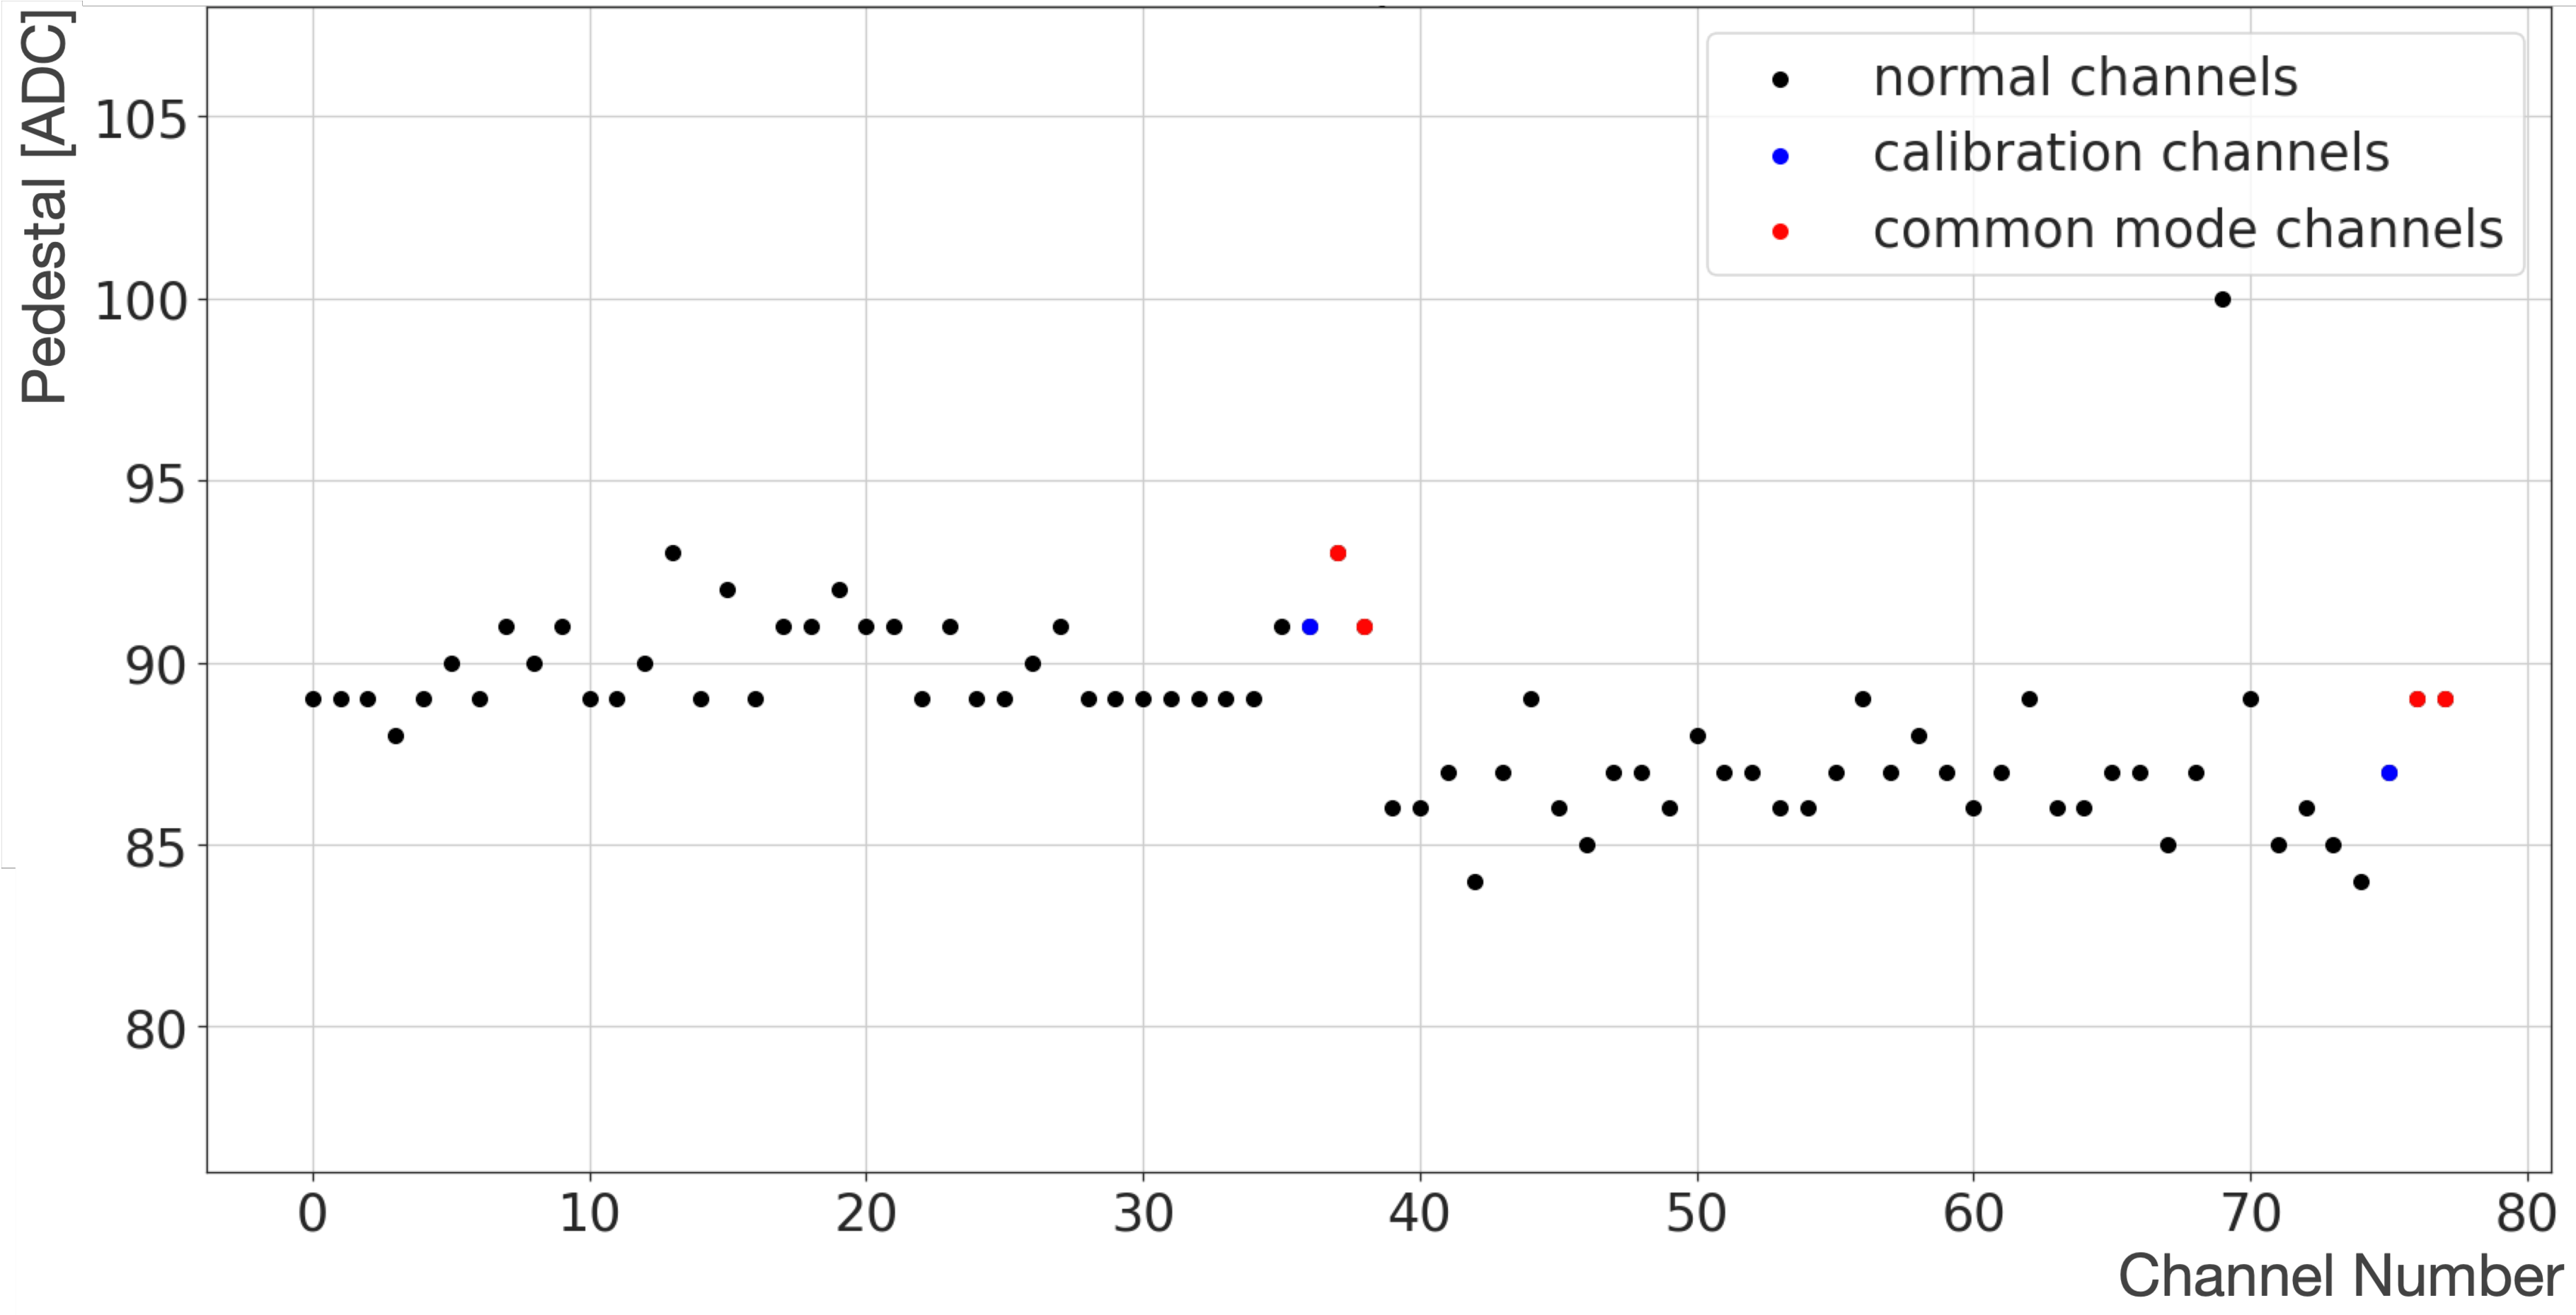
\includegraphics[width=0.49\linewidth]{Figures/HGCAL/Pedestal_1.pdf}
    \caption{Pedestal values of the HGCROC3 channels before (left) and after (right) the pedestal calibration procedure: channel numbers from 0 to 39 belong to the first half, channel numbers from 40 to 77 belong to the second half of the chip. The main target of the calibration is to reduce the dispersion between the channels and minimise their average.}
    \label{fig:Pedestal}
\end{figure}

\begin{figure}
    \centering
    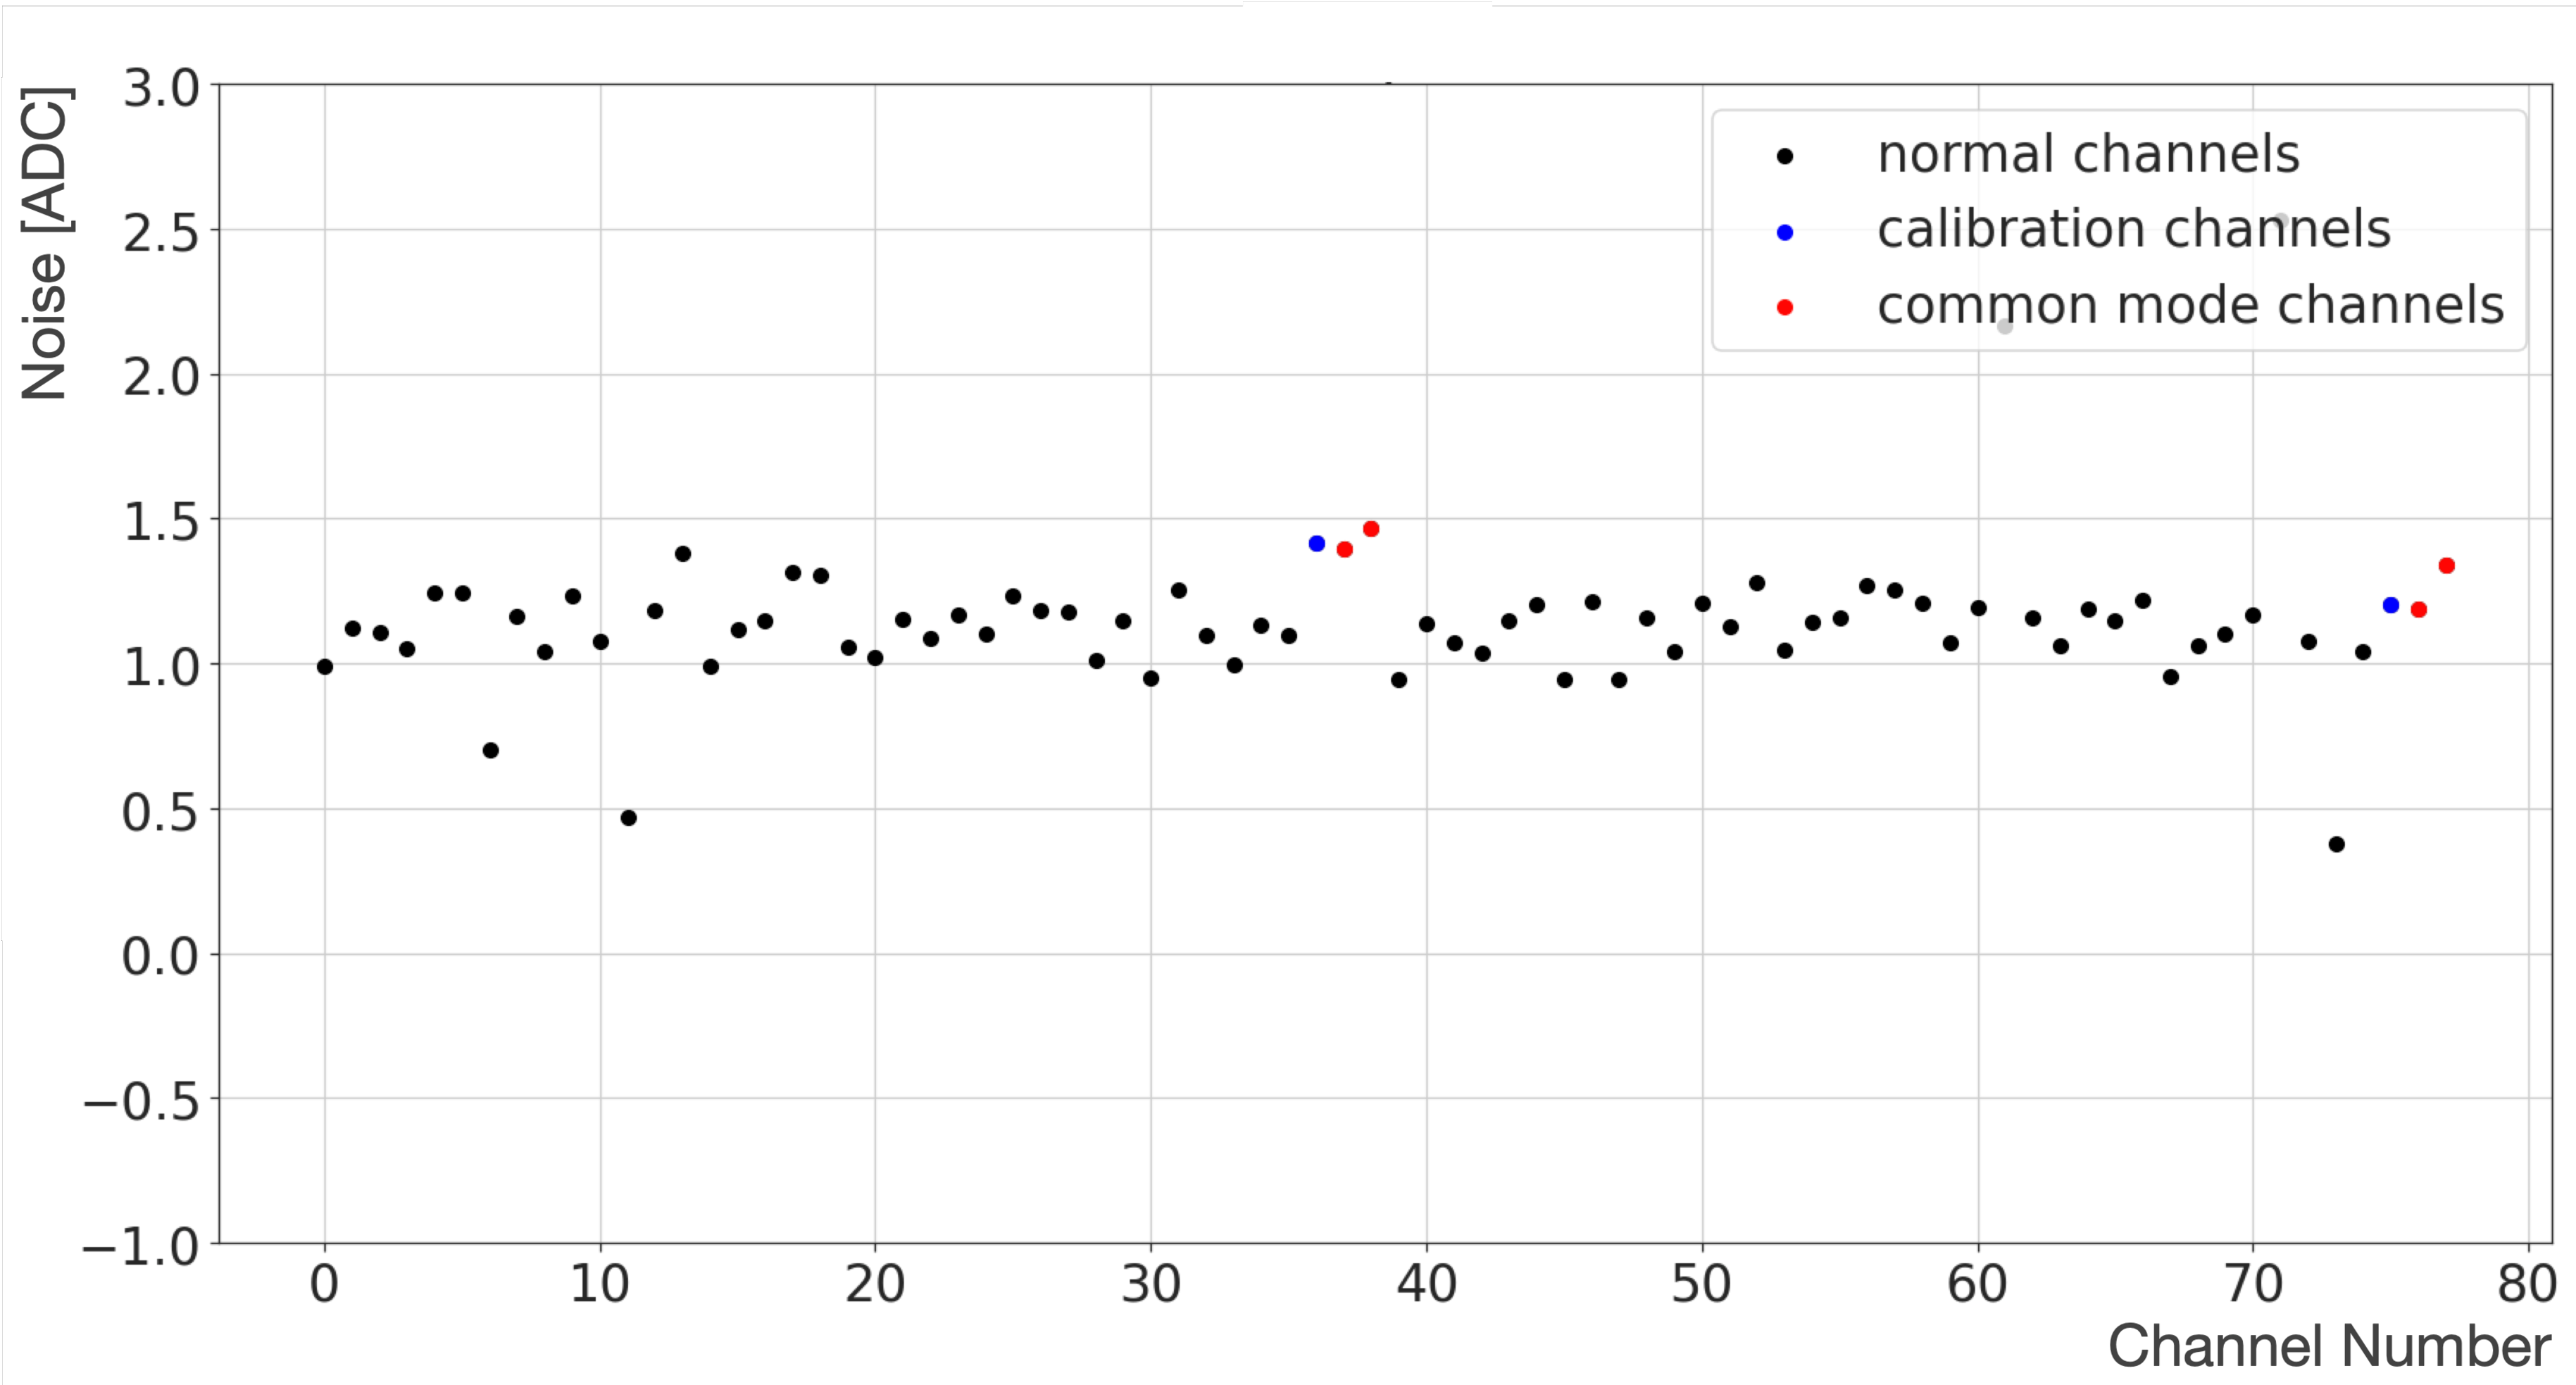
\includegraphics[width=0.49\linewidth]{Figures/HGCAL/Noise_0.pdf}
    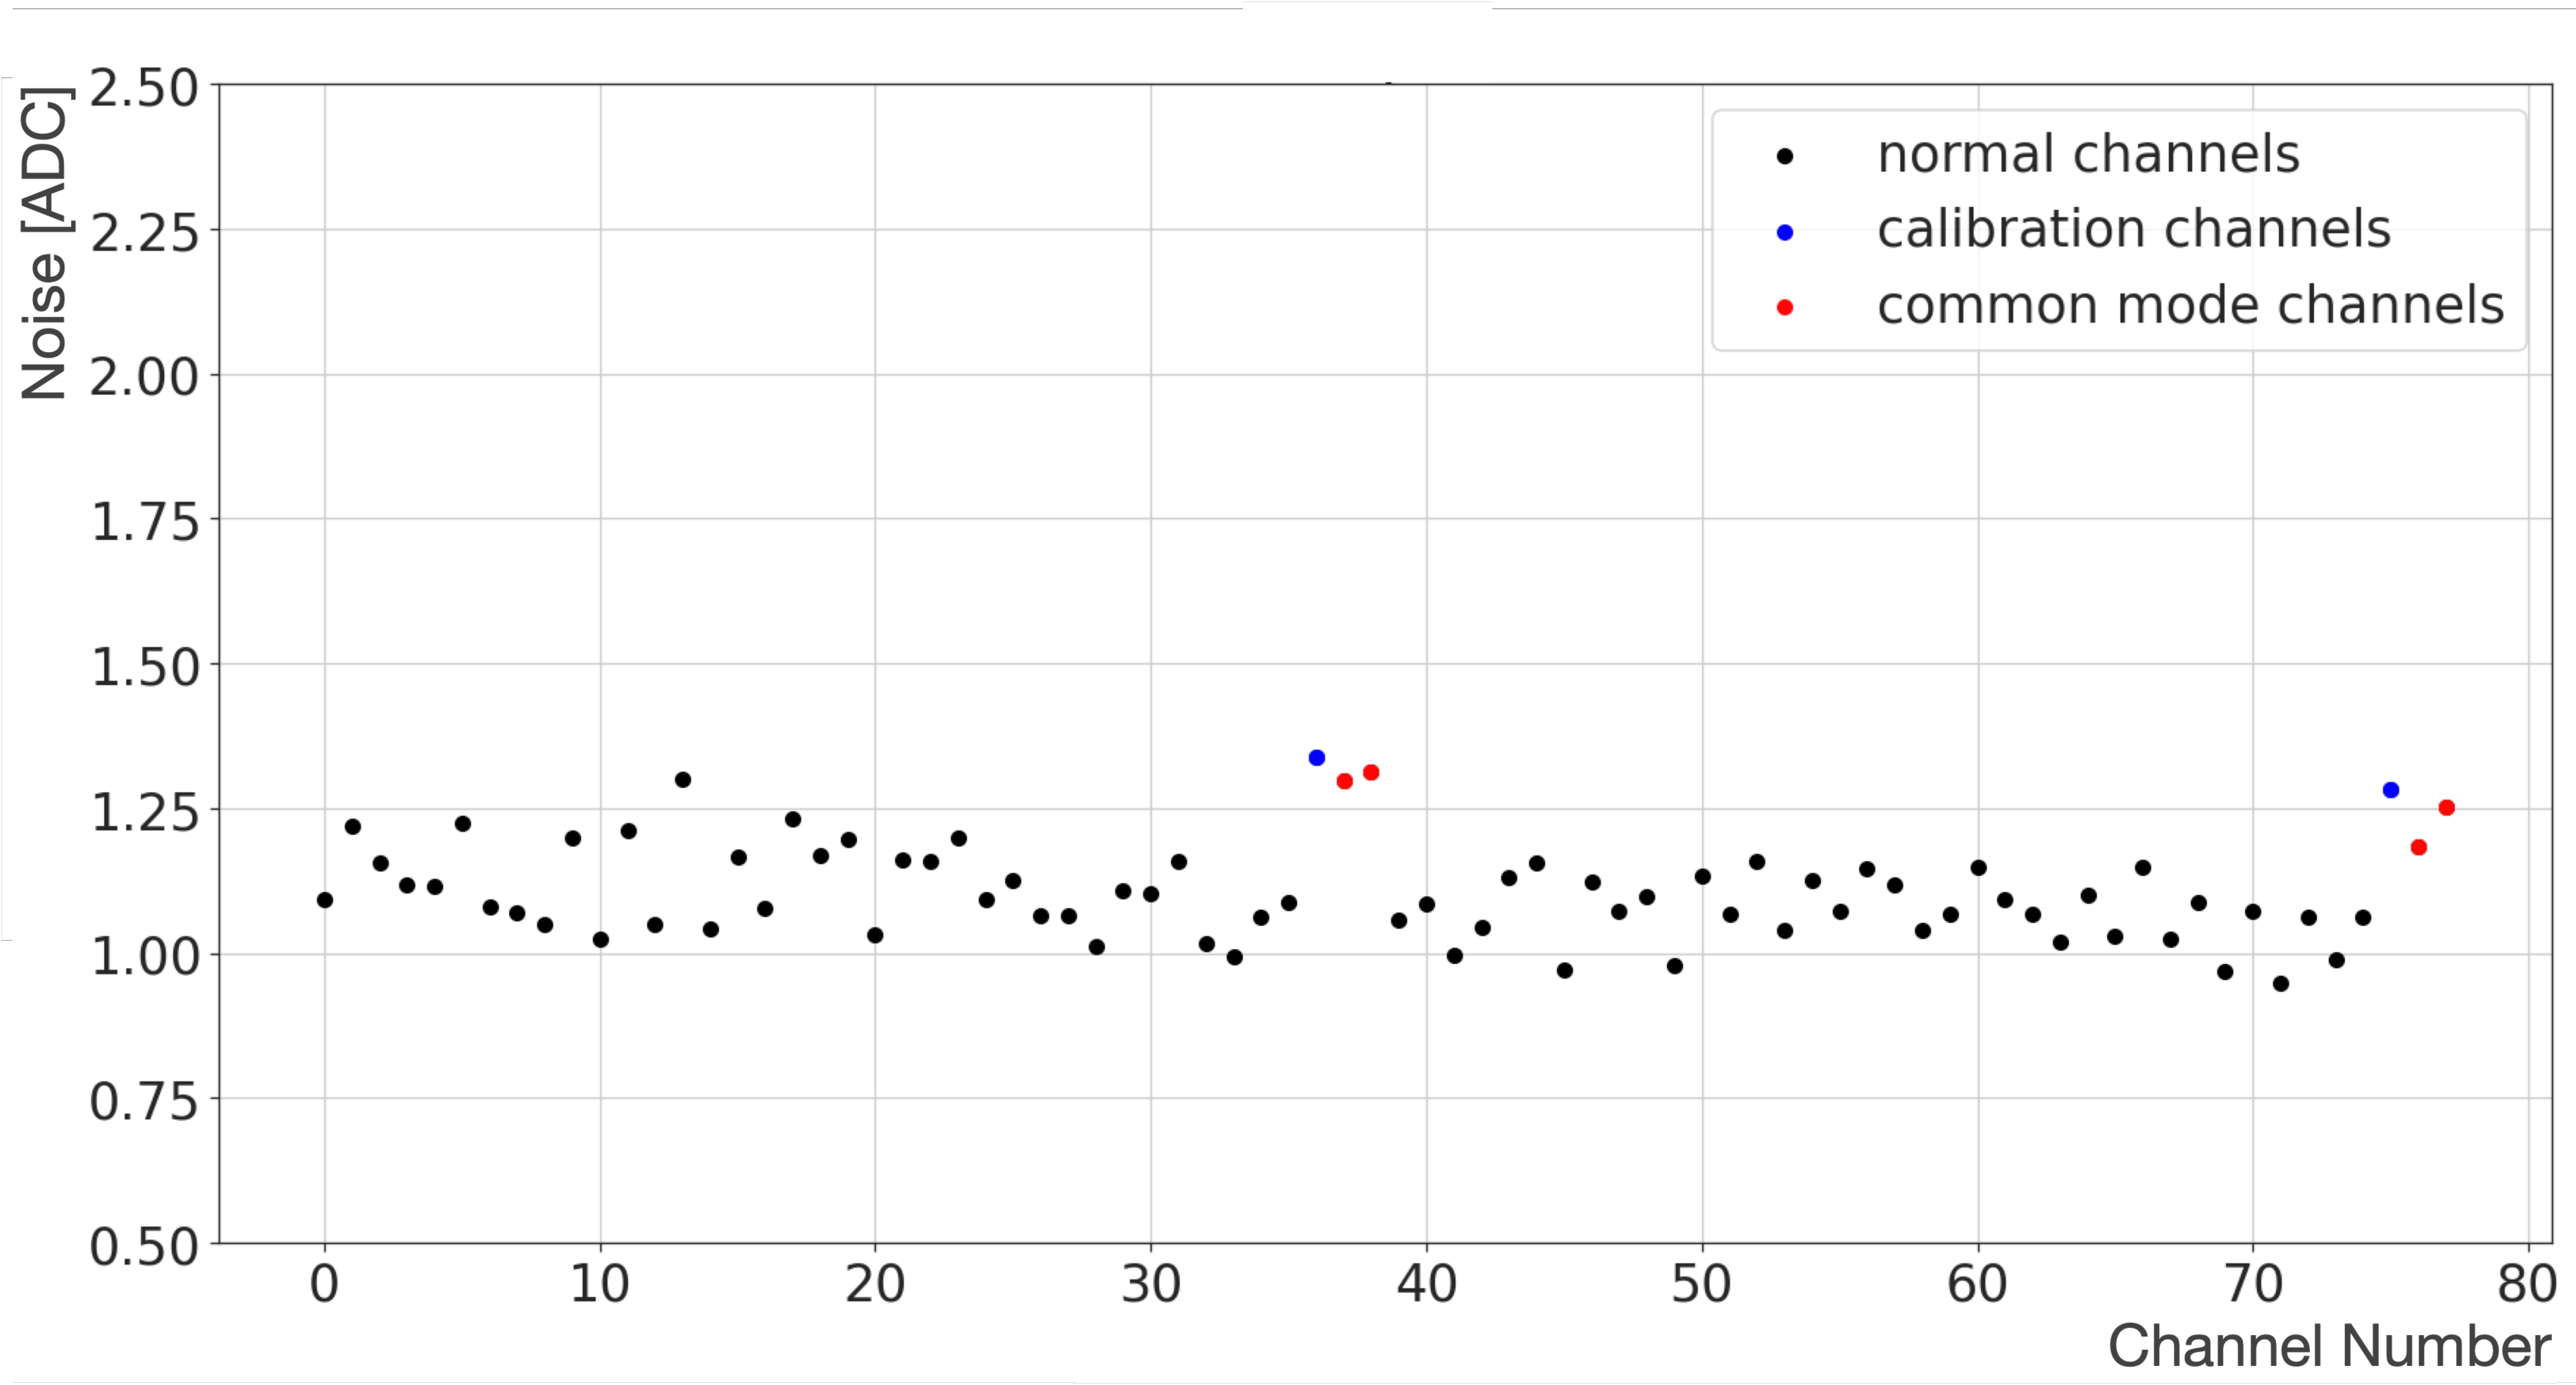
\includegraphics[width=0.49\linewidth]{Figures/HGCAL/Noise_1.pdf}
    \caption{Noise values of the HGCROC3 channels before (left) and after (right) the pedestal calibration procedure: channel numbers from 0 to 39 belong to the first half, channel numbers from 40 to 77 belong to the second half of the chip. The pedestal calibration also aims at minimising the electronic noise of the channels.}
    \label{fig:Noise}
\end{figure}

\begin{figure} 
    \centering
    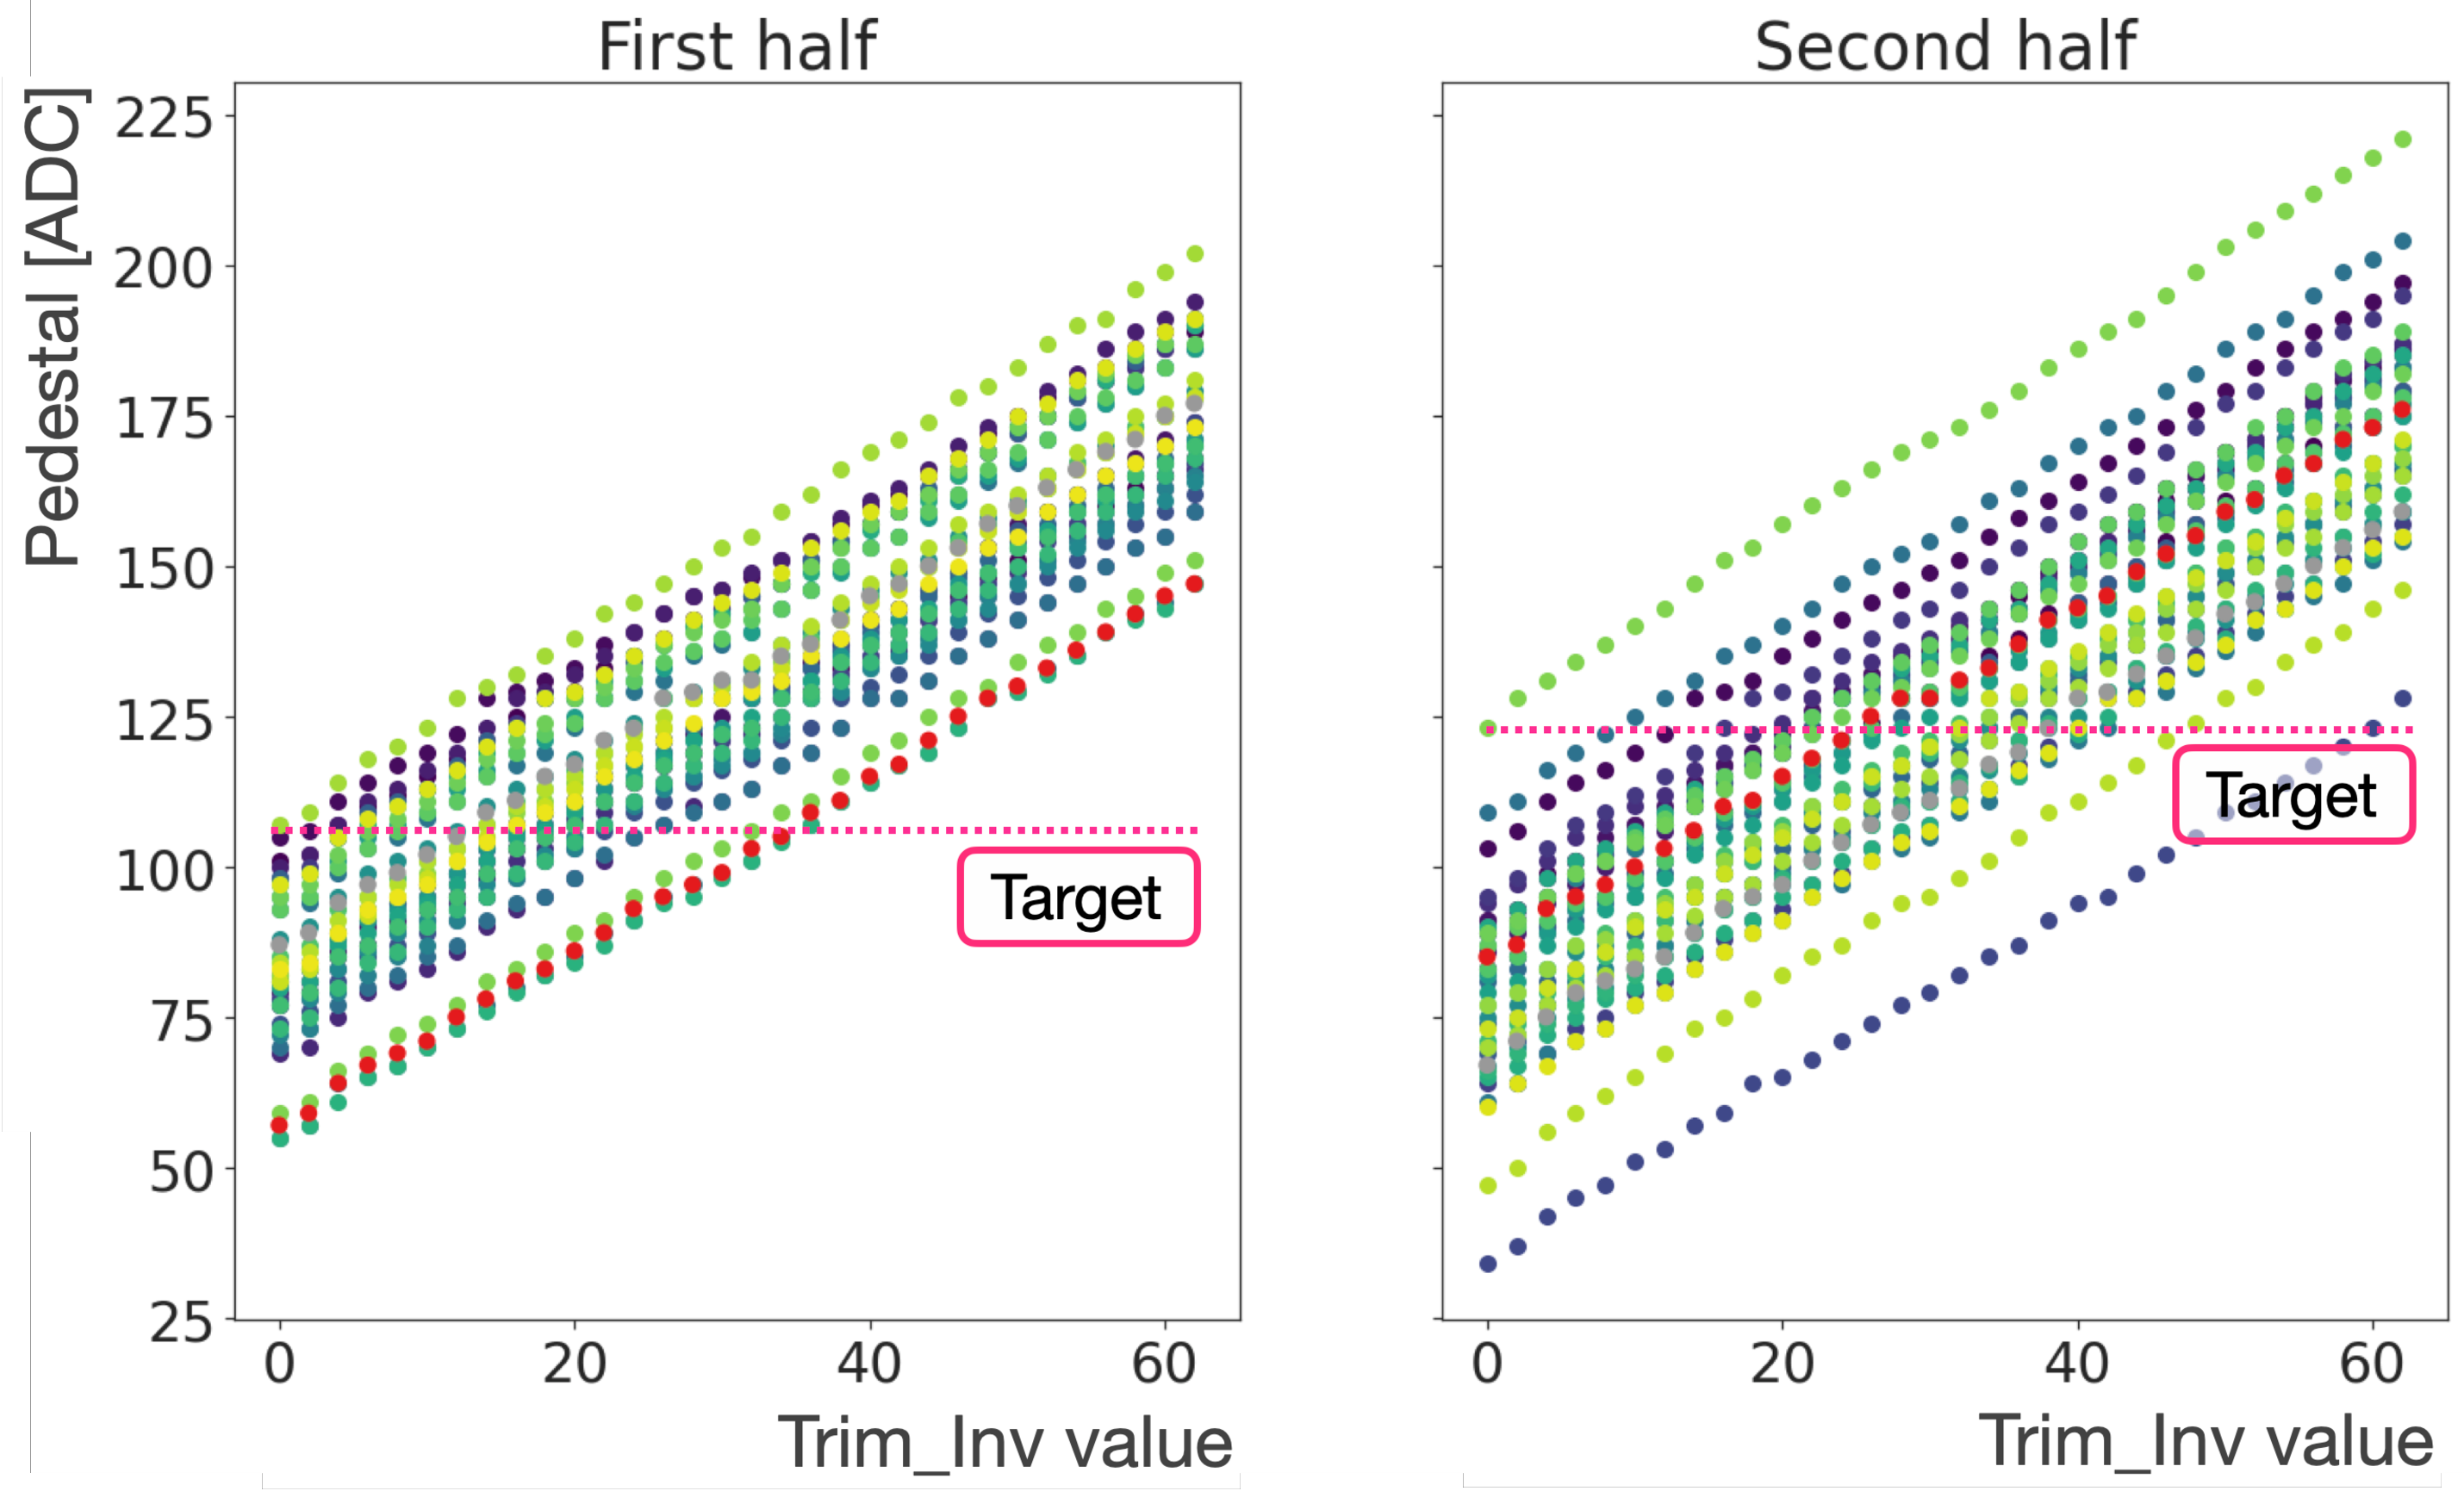
\includegraphics[width=0.7\linewidth]{Figures/HGCAL/PedestalScan.pdf}
    \caption{Pedestal values of the HGCROC3 channels as a function of the \texttt{Trim\_Inv} parameter, used for a channel-wise pedestal trimming.}
    \label{fig:PedestalScan}
\end{figure}

\bigbreak

Once each half shows a similar pedestal value in all channels, a \textit{global} pedestal trimming is performed to lower down the pedestal value to approximately 10~ADC and fully exploit the 1~V digitisation range.
The global pedestal value is configurable through two per-half parameters, \texttt{Vref\_Inv} and \texttt{Vref\_NoInv}, in such a way that the 1~V signal range is placed at the center of the 1.2~V dynamic range of the chip.
The configuration of the pedestal value depends on the expected noise levels and ground fluctuations of the testing set-up: in the batch testing experimental conditions, high fluctuations of the ground potential are expected, for this reason the pedestal value is set to a slightly higher level around 50~ADC in order to maintain a discrete margin.

\bigbreak

The final configuration of the pedestal values for the 78 channels, after the pedestal calibration procedure is show in the right plot of Figure~\ref{fig:Pedestal}. The electronic noise of each channel before and after the pedestal calibration is also shown in Figure~\ref{fig:Noise}.

% Since the analog part of the HGCROC3 is powered at 1.2~V, two per-half parameters are present in the I2C register to place the signal range at the center of the dynamic range.
% In order to better understand this procedure, it is useful to go a bit in the details of the ADC chain. Before the preamplified analog signal enters the ADC block, it is split in two signals with same shape and opposite polarisation: the positively polarised signal enters the \textit{Non Inverted} chain, while the negatively polarised signal enters the \textit{Inverted} chain. Both chains have a 1.2~V dynamic range.
% It is possible to change the values of Vref_inv and Vref_noinv in 10b-DACs (1024 values) to find the best combination. The principle is to force one of the ADC input to 0.6 V (half of the signal range), perform a scan of the Vref DAC of the other branch and set it to the value giving the code 256 ADC (266 in fact to have some margin), and then redo the same operation but for the other branch. By construction, this procedure allows the optimization of both the pedestal and the dynamic range. 

\subsubsection{The time thresholds calibration}
\label{subsubsec:The time thresholds calibration}

The Time-of-Arrival (ToA) denotes the timing measurement of the signal, determined by the moment when the signal amplitude surpasses a predefined threshold value. The ToA threshold should be calibrated slightly above the pedestal level to ensure accurate timing acquisition for the majority of the events. Moreover, the read-out chip should provide the same timing efficiency across different modules and channels, without being affected by fluctuations in the pedestal or noise values.

\bigbreak

In the HGCROC3, two channel-wise parameters (\texttt{ToA\_Vref} and \texttt{Trim\_ToA}) are available to calibrate the ToA thresholds in order to minimise the ToA efficiency dispersion among channels.
For the ToA calibration, a small charge with a fixed ADC amplitude is internally injected into each channel and a scan of different discriminator thresholds is performed. For each threshold, the ToA efficiency is computed, defined as the ratio of ToA triggers to the total number of injected events: if the threshold is low, all events will trigger a ToA signal and the efficiency will be equal to 1, while if the threshold is high, no event will reach the discriminator and the efficiency will be 0.

The ToA efficiency as a function of the different threshold values is presented in the left plot of Figure~\ref{fig:ToAEff} before the calibration procedure.
The goal of the ToA threshold calibration is to have, for a given \texttt{ToA\_Vref} value, the same ToA efficiency in all channels. 
Since the value of the discriminator threshold is defined as the difference between \texttt{ToA\_Vref} and \texttt{Trim\_ToA}, it is possible to configure the channel-wise \texttt{Trim\_ToA} so that the the 50$\%$ efficiency is reached for the same \texttt{ToA\_Vref} value for all channels: the final performance after the calibration procedure is shown in the right plot of Figure~\ref{fig:ToAEff}.

\bigbreak

The Time-over-Threshold (ToT) is a method to provide an estimation of the signal amplitude for very high pulses that saturate the ADC dynamic range by measuring the duration of the signal pulse saturation. 
The ToT is computed only for pulses exceeding the ToT threshold, that needs to be configured below the preamplifier saturation point, in order not to have gaps between the ADC and the ToT dynamic range of measurements. The process of establishing the ToT threshold voltage is similar to the ToA calibration method, and is configurable through equivalent channel-wise parameters, \texttt{ToT\_Vref} and \texttt{Trim\_ToT}.

\begin{figure}
    \centering
    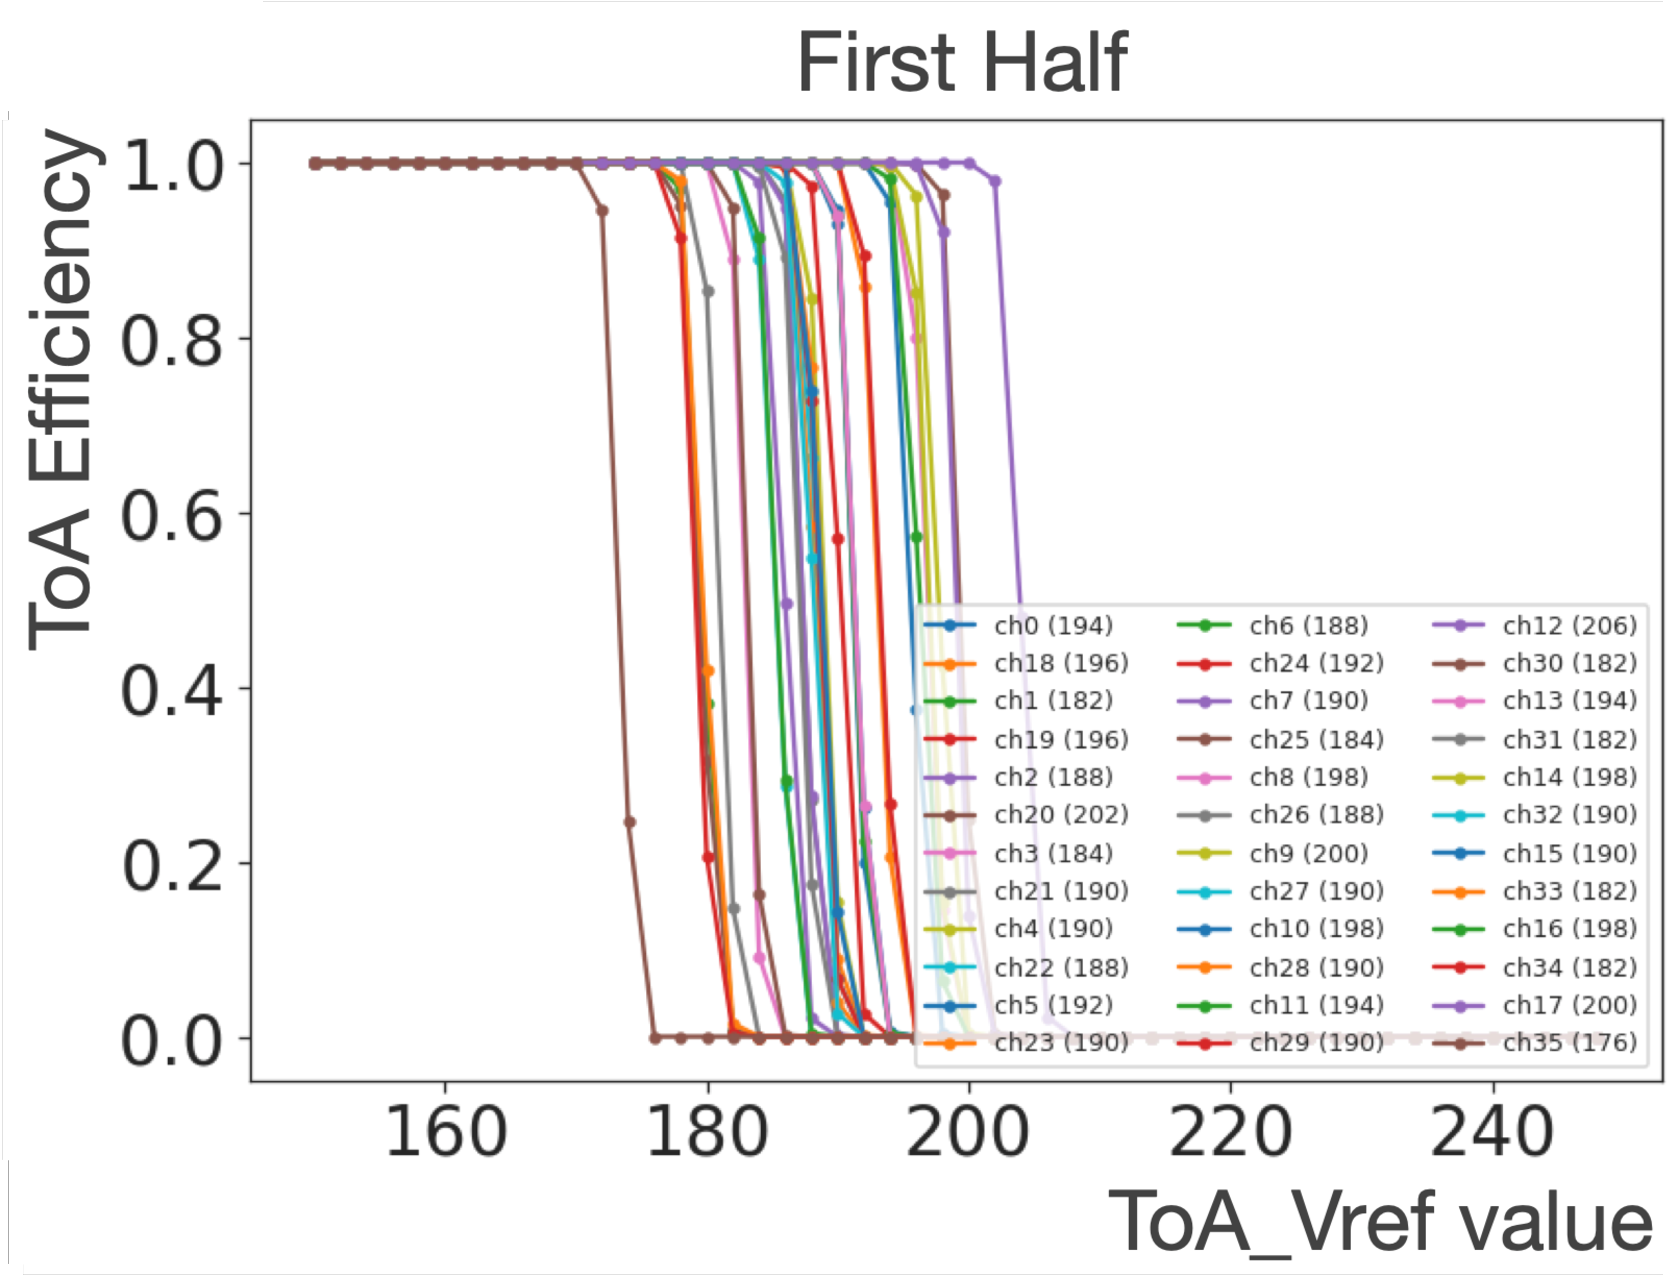
\includegraphics[width=0.49\linewidth]{Figures/HGCAL/ToA_Eff_0.pdf}
    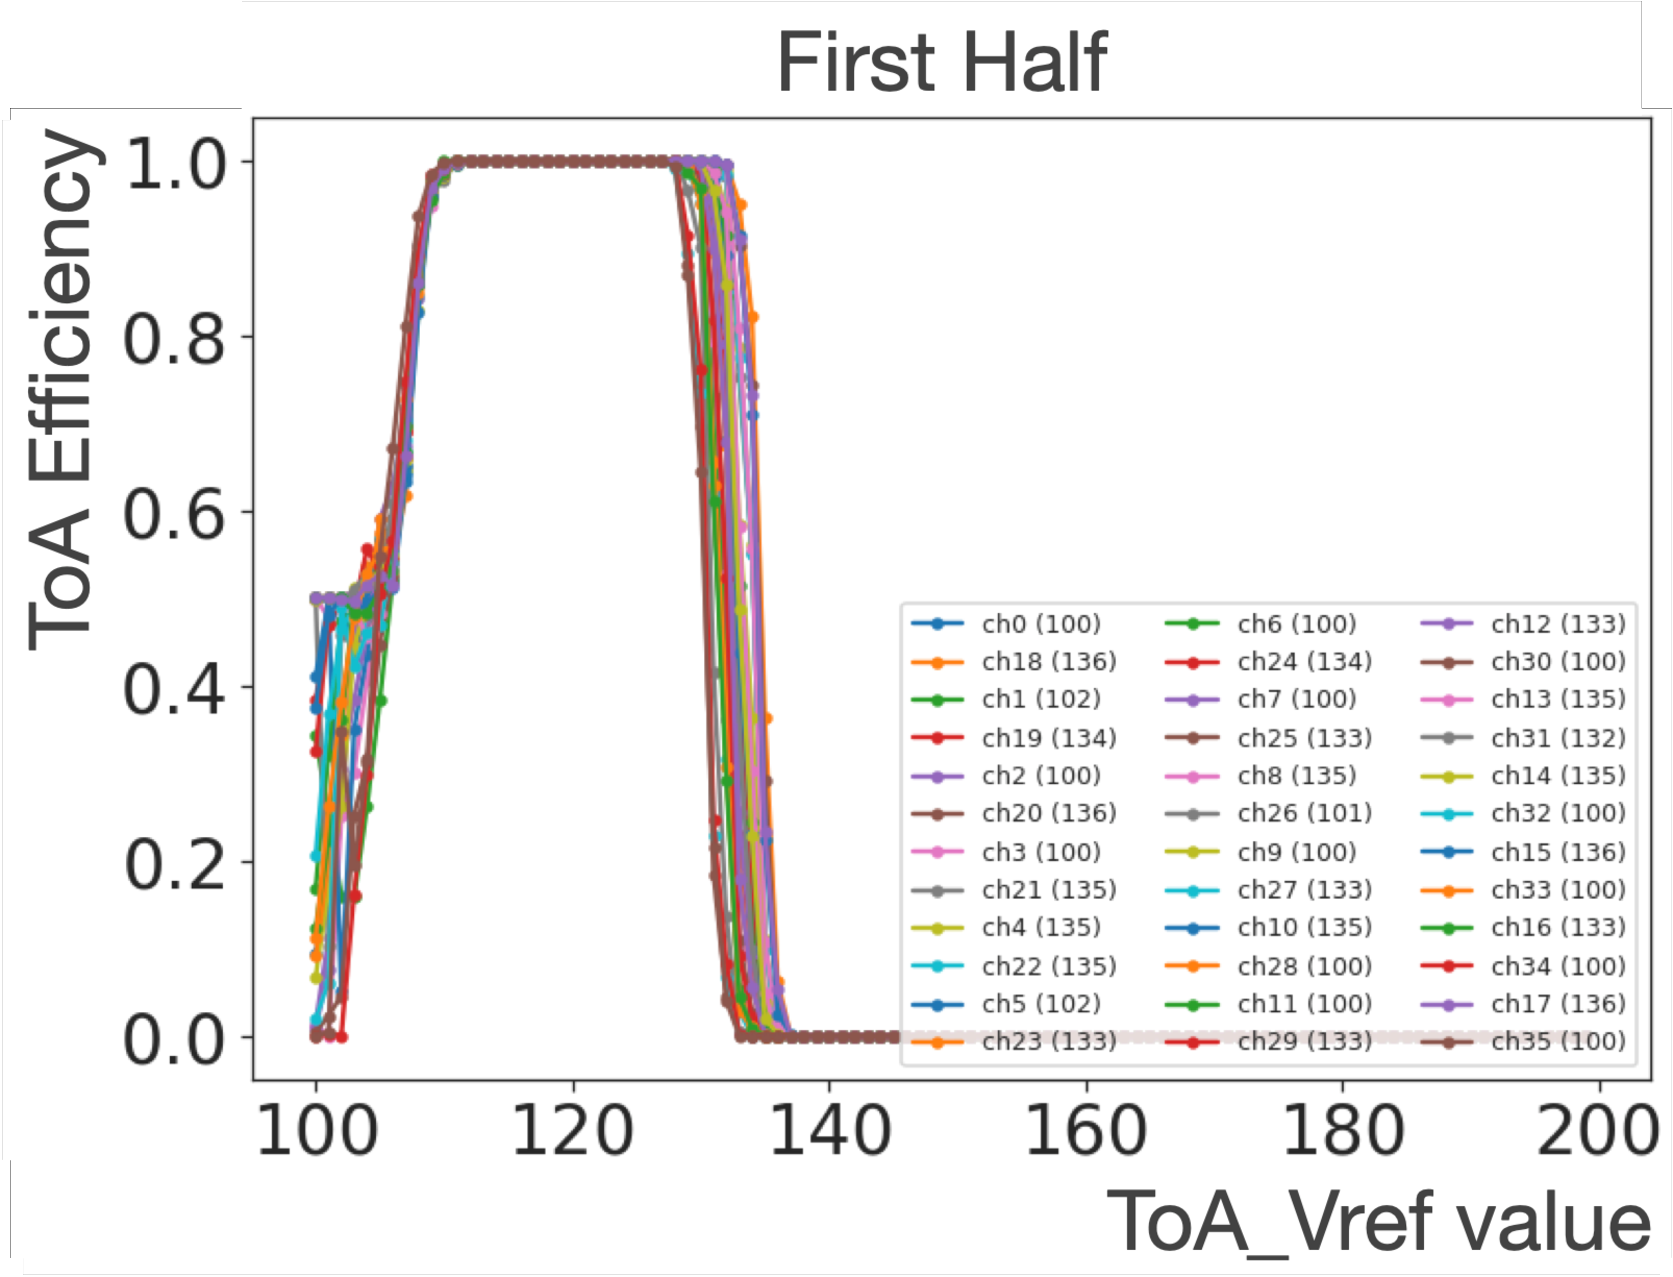
\includegraphics[width=0.49\linewidth]{Figures/HGCAL/ToA_Eff_1.pdf}
    \caption{ToA efficiency, defined as the ratio between ToA triggered events and total number of injected events, as a function of the \texttt{ToA\_Vref} parameter, defining the ToA discriminator threshold, before (left) and after (right) the ToA threshold calibration procedure.}
    \label{fig:ToAEff}
\end{figure}

% The ToA injection scan measures the time of arrival of the signal. The ToA is the instant of time at which the signal amplitude exceeds a threshold value. You can see from the example that a smaller signal amplitude provides a bigger ToA, while a higher signal amplitude leads to a smaller ToA. This is reflected in the right plot, where we can see the so-called “time walk”.

\subsubsection{The phase calibration}
\label{subsubsec:The phase calibration}

In order to correctly measure the amplitude of the physical signal, the ADC and TDC conversion blocks of the HGCROC3 are provided with an adjustable sampling phase parameter.
Each 25~ns bunch crossing (BX) period is internally sampled into 16 phases: each ASIC can be configured in such a way that the signal amplitude is sampled at the correct phase, which might depend on the rapidity angle of the module and on the silicon sensor thickness.

Figure~\ref{fig:BestPhase} shows a scan over phases of the ADC value that reconstructs the signal shape of an injected pulse: in this case, the sampling phase corresponding to the signal peak is determined to be phase 0.
The signal sampling also shows an oscillation in the pedestal value, due to the fluctuation of the ground potential.
% , that can be subtracted through the common mode channels.
%  check with Glen, CM channels used for HV noise and others

\begin{figure}[b!]
    \centering
    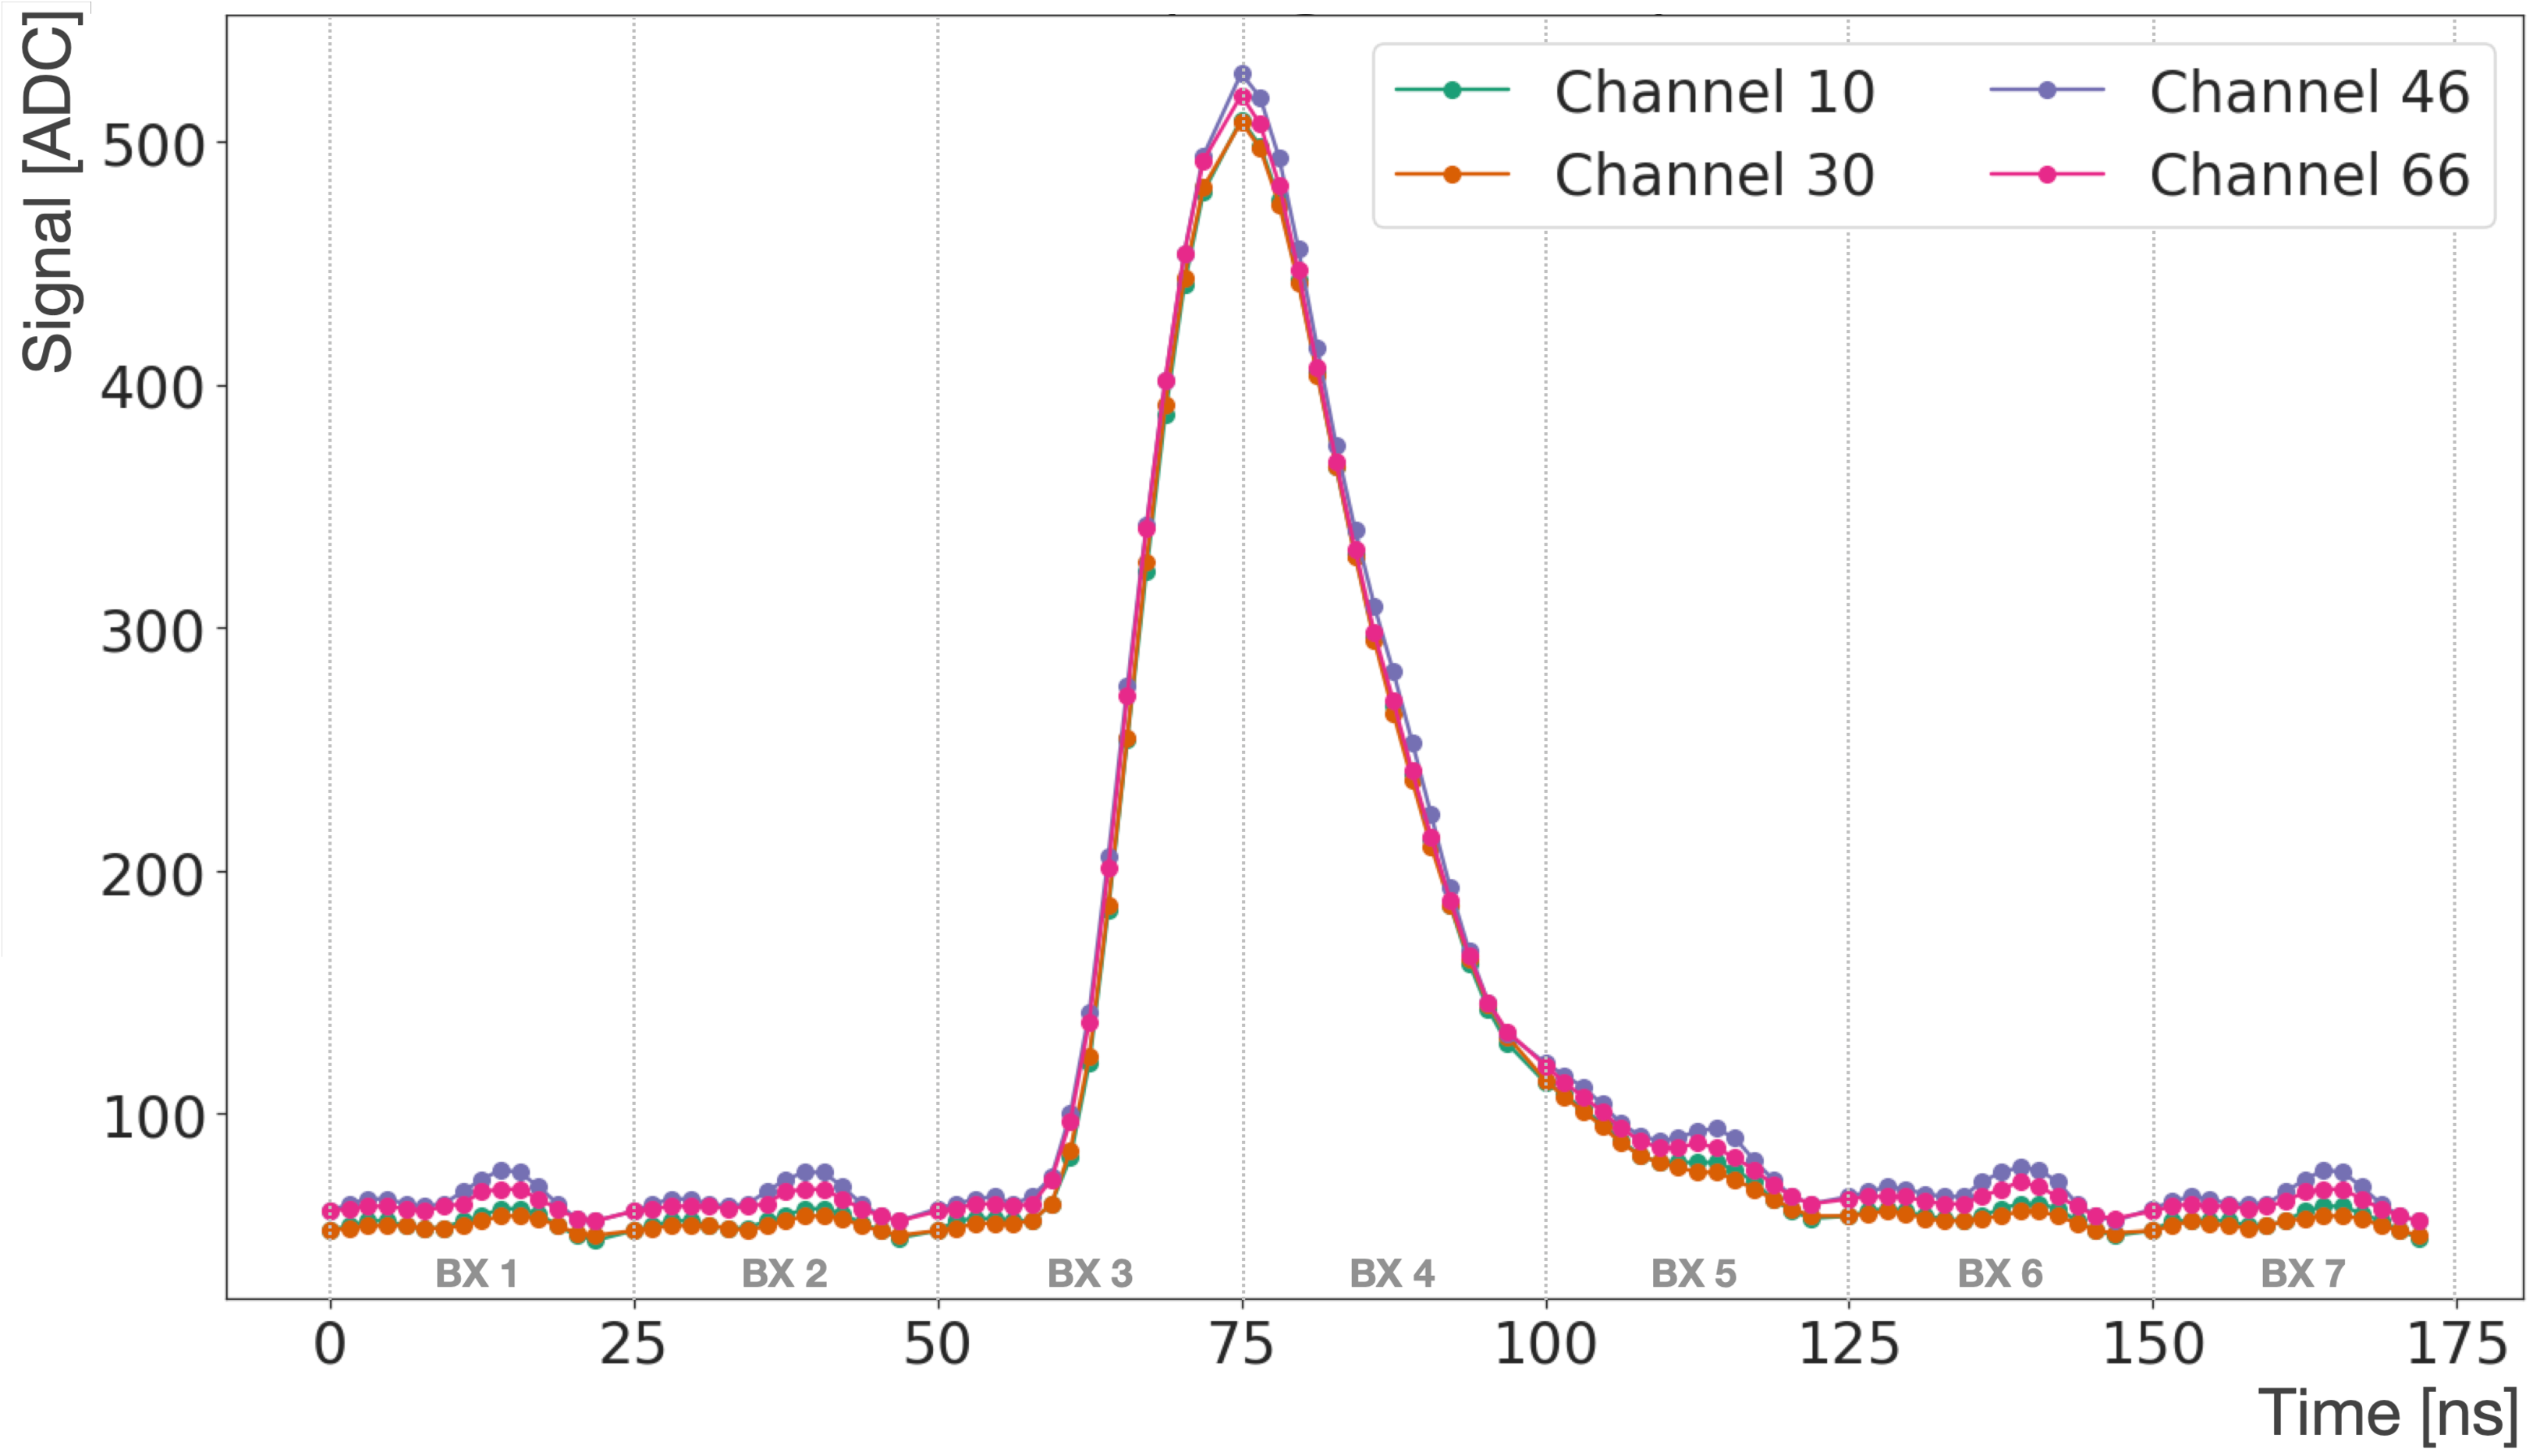
\includegraphics[width=0.65\linewidth]{Figures/HGCAL/BestPhase.pdf}
    \caption{Sampling scan of the ADC value of 4 channels for different phases. Each 25~ns bunch crossing (BX) period is divided into 16 phases: the sampling position is determined by the phase of the signal maximum.}
    \label{fig:BestPhase}
\end{figure}

\bigbreak

Other configurable parameters exist within the HGCROC3 I2C register, but are not addressed in this context as they are not relevant in this thesis work.

\subsection{The HGCROC3 performance}
\label{subsec:The HGCROC3 performance}

Once the HGCROC3 is correctly configured for the data acquisition, it is possible to check that its performance aligns with the HGCAL FE electronics requirements.

The ASIC can measure charges spanning from 160~fC to 320~pC, with two different regimes: the ADC is calibrated to accurately detect charges up to the preamplifier saturation, when the saturation is reached the Time-Over-Threshold (ToT) technique measures the signal duration over saturation. The transition from ADC to ToT is configurable through the I2C parameters. The preamplifier output is also connected to the Time-Of-Arrival (ToA) discriminator to capture timing information. 

Considering the various types of signal pulses to be read out by the HGCROC3, it is essential to evaluate the response of the device to different signal amplitudes in terms of ADC, ToA and ToT.

\subsubsection{The ADC performance}
\label{subsubsec:The ADC performance}

The front-end ADC operates at 40 MHz to convert the analog signal into a digitised value corresponding to the signal amplitude and consequently to energy deposit in the detector. 
Figure~\ref{fig:FitSampling} shows a typical signal pulse recorder by the HGCROC3 and modeled by the following equation:

\begin{equation}
    f(t) = A_{0}\,e^{-at}\left[e^{-ct}\left(\frac{t^3}{c}-\frac{3t^2}{c^2}+\frac{6t}{c^3}-\frac{6}{c^4}\right)+\frac{6}{c^4}\right], \;\; a =\frac{1}{\tau_{p}}, \;\; c=\frac{1}{\tau_{p}}-\frac{1}{\tau_{s}}
\label{eq:FitSampling}
\end{equation}
where $\tau_{p}$ and $\tau_{s}$ correspond to the characteristic time of the preamplifier and of the shaper circuit respectively.
The model well describes the recorded data, with minor discrepancies below 2\%.

\begin{figure}
    \centering
    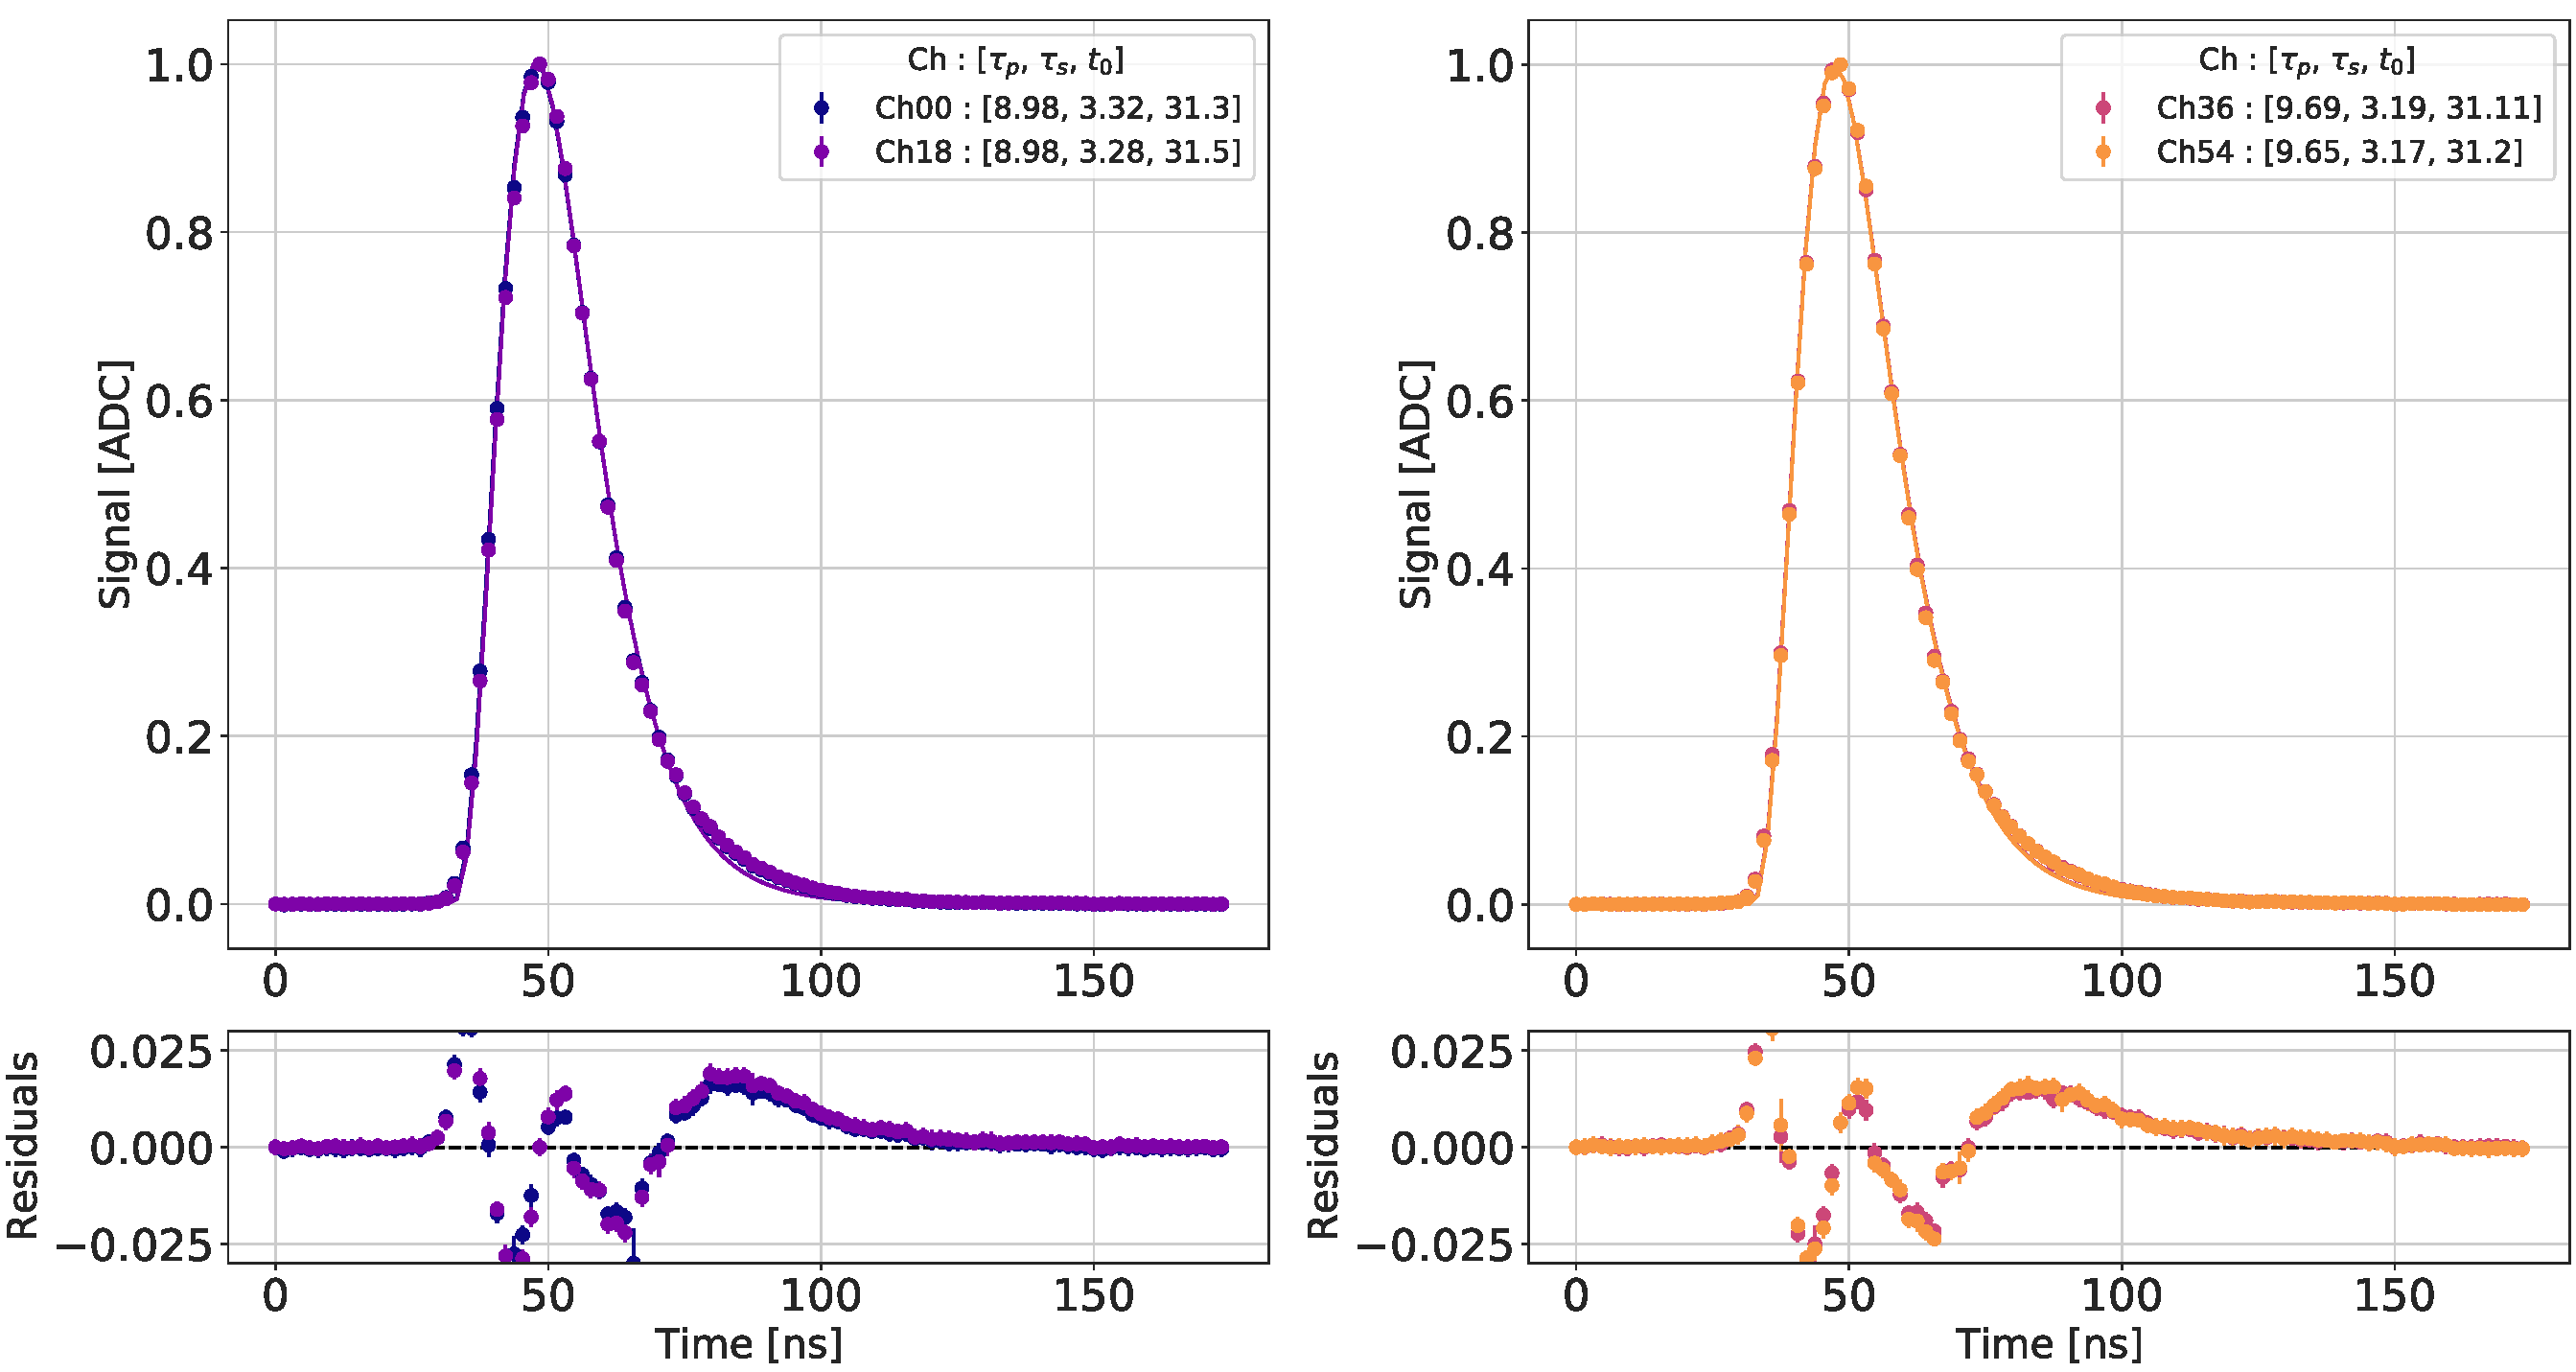
\includegraphics[width=0.75\linewidth]{Figures/HGCAL/FitSampling.pdf}
    \caption{Normalised signal pulse for 4 channels of the HGCROC3, two channels of the first half (left) and two channels of the second half (right). The signal shape is fitted using Equation~\ref{eq:FitSampling} and the optimised parameters of the fit are reported in the legend. Discrepancies between the model and the data are below 2\%.}
    \label{fig:FitSampling}
\end{figure}

\bigbreak

A high linearity is crucial for the ADC to accurately extract the signal amplitude and ensure a precise charge measurements. The ADC performance is tested by injecting signals with increasing charge value and verifying the linearity of the recorded ADC as a function of the input charge. Figure~\ref{fig:ADC_Injection} shows the expected linear response of the signal amplitude measured by the HGCROC3 with respect to the injected charge, in units of the \texttt{Calib\_DAC} parameter - 100~\texttt{Calib\_DAC} corresponds to a charge of 120~fC. The linear function described in Equation~\ref{eq:ADCLinearity} is used to test the linearity of the response and the best parameters extracted from the fit are reported in the legend for each channel.

\begin{equation}
    f(t) = ax + b
\label{eq:ADCLinearity}
\end{equation}

\begin{figure}
    \centering
    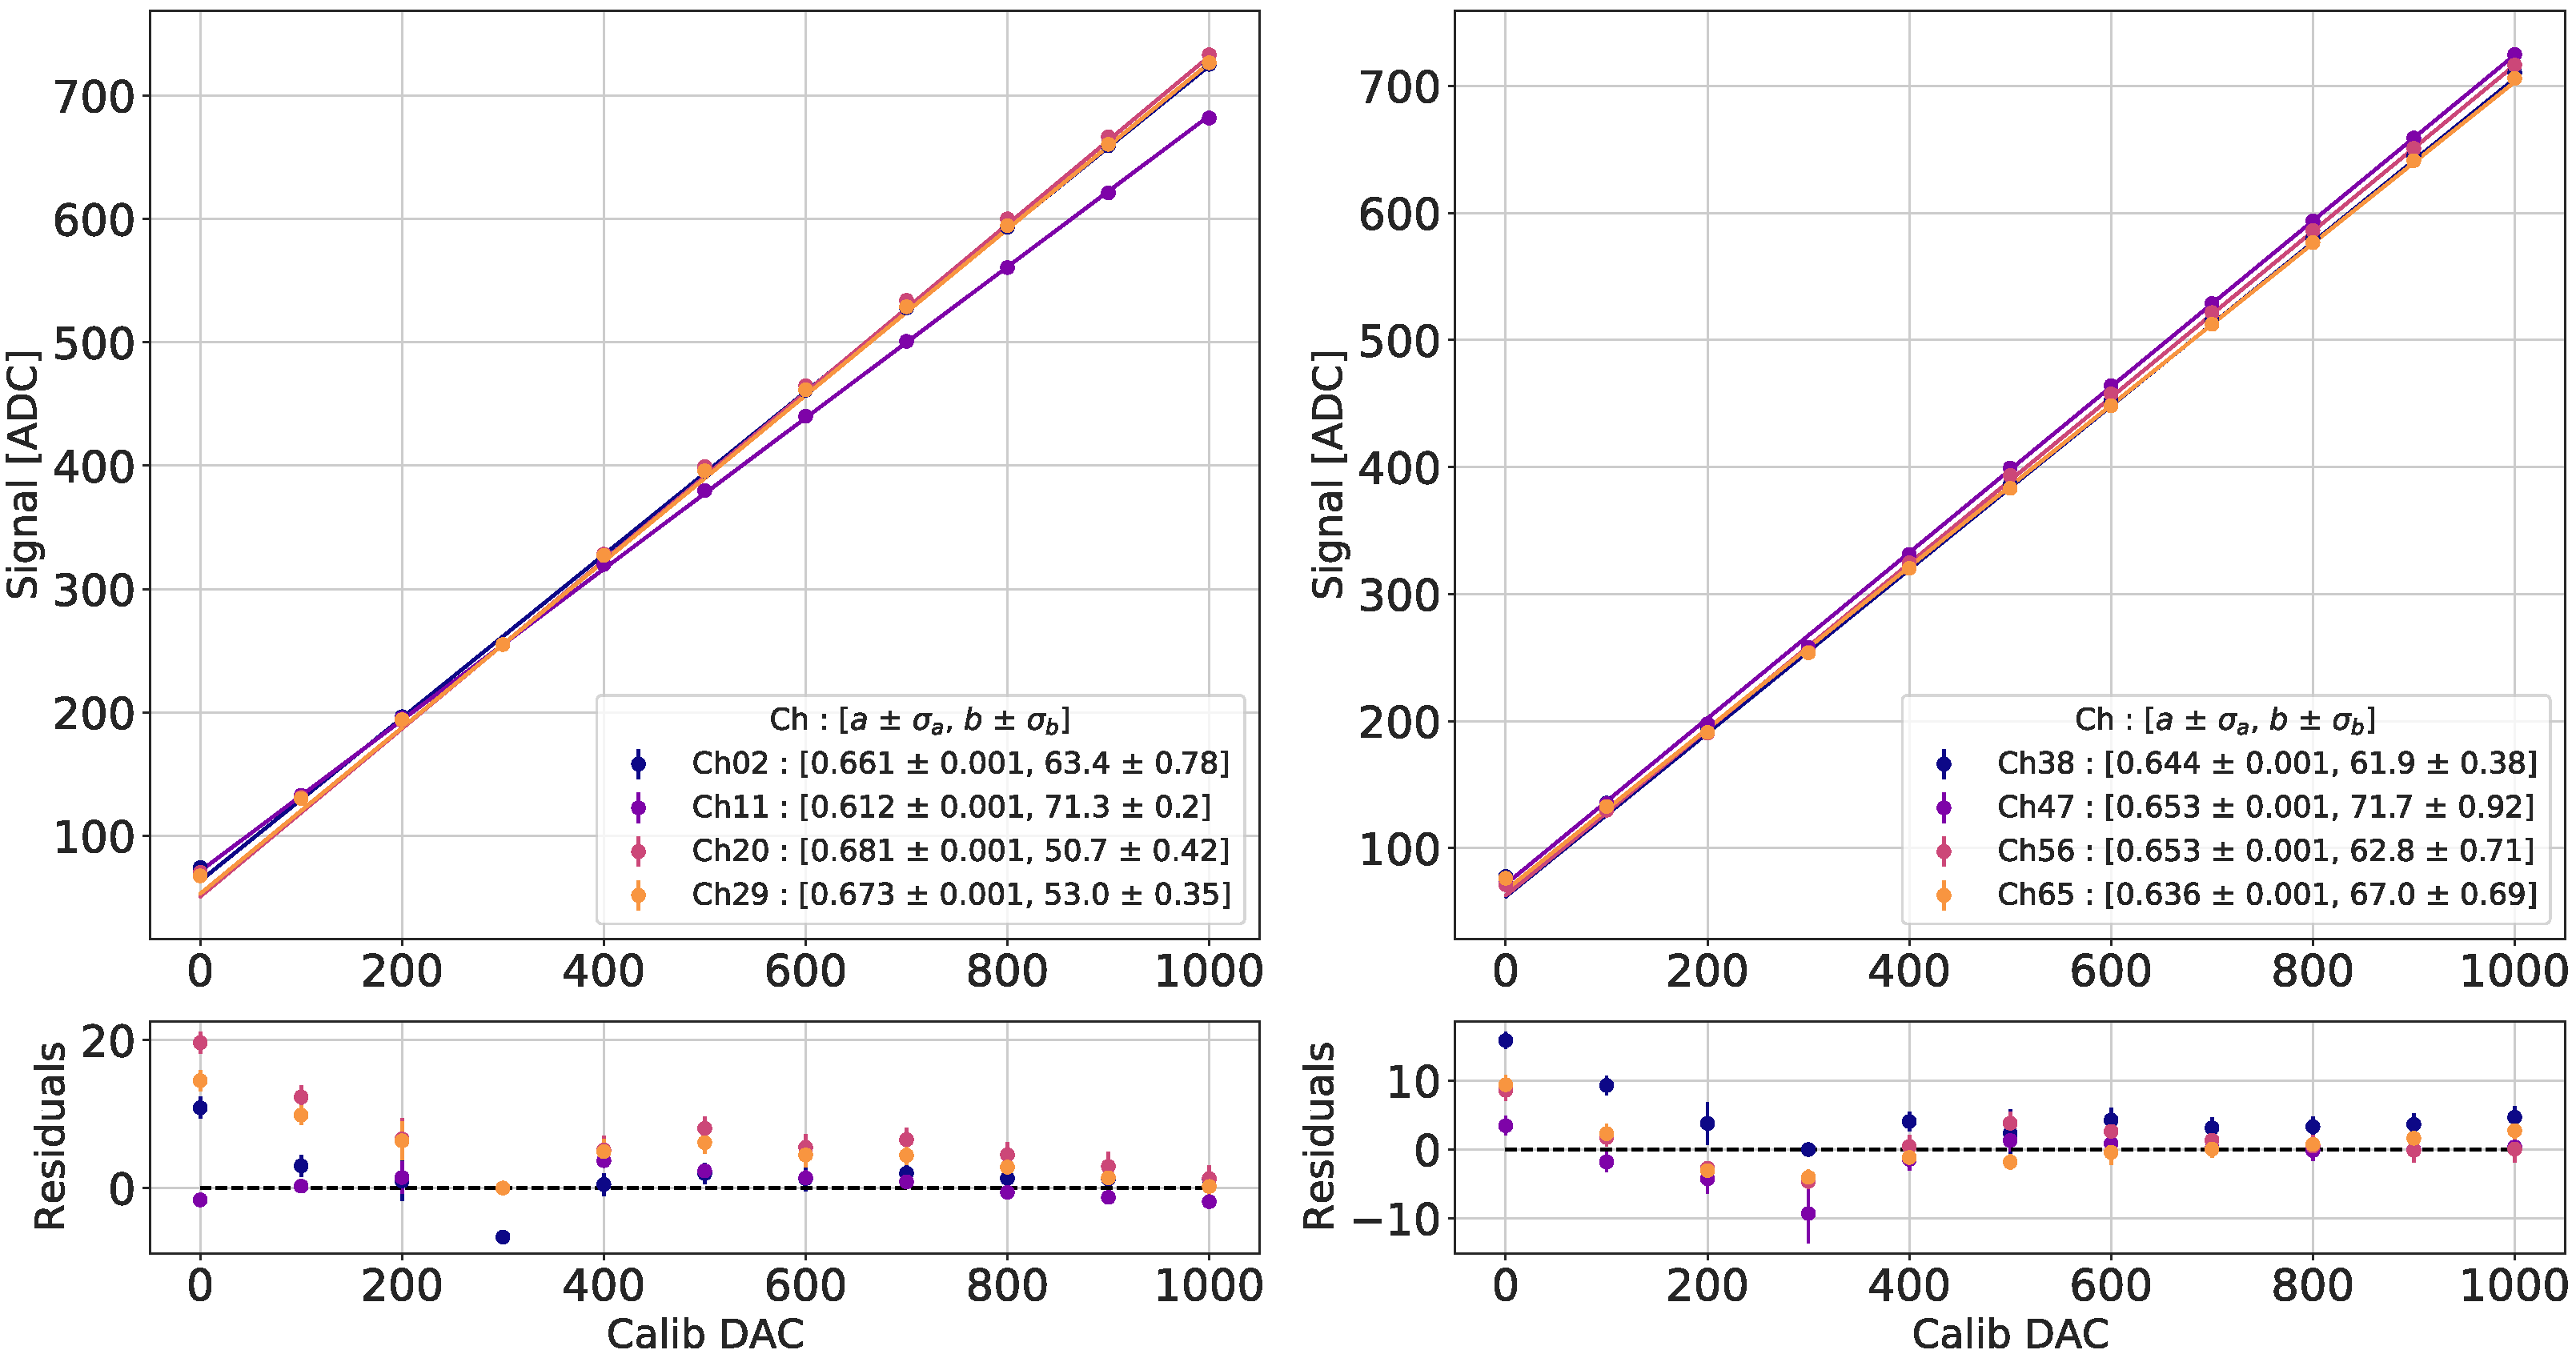
\includegraphics[width=0.75\linewidth]{Figures/HGCAL/ADC_Injection.pdf}
    \caption{The ADC response linearity to multiple injections corresponding to different \texttt{Calib\_DAC} values, defining the input charge. The  response is fitted with the linear function in Equation~\ref{eq:ADCLinearity} and the optimised parameters of the fit are reported in the legend.}
    \label{fig:ADC_Injection}
\end{figure}

\subsubsection{The ToT performance}
\label{subsubsec:The ToT performance}

\begin{figure}[b!]
    \centering
    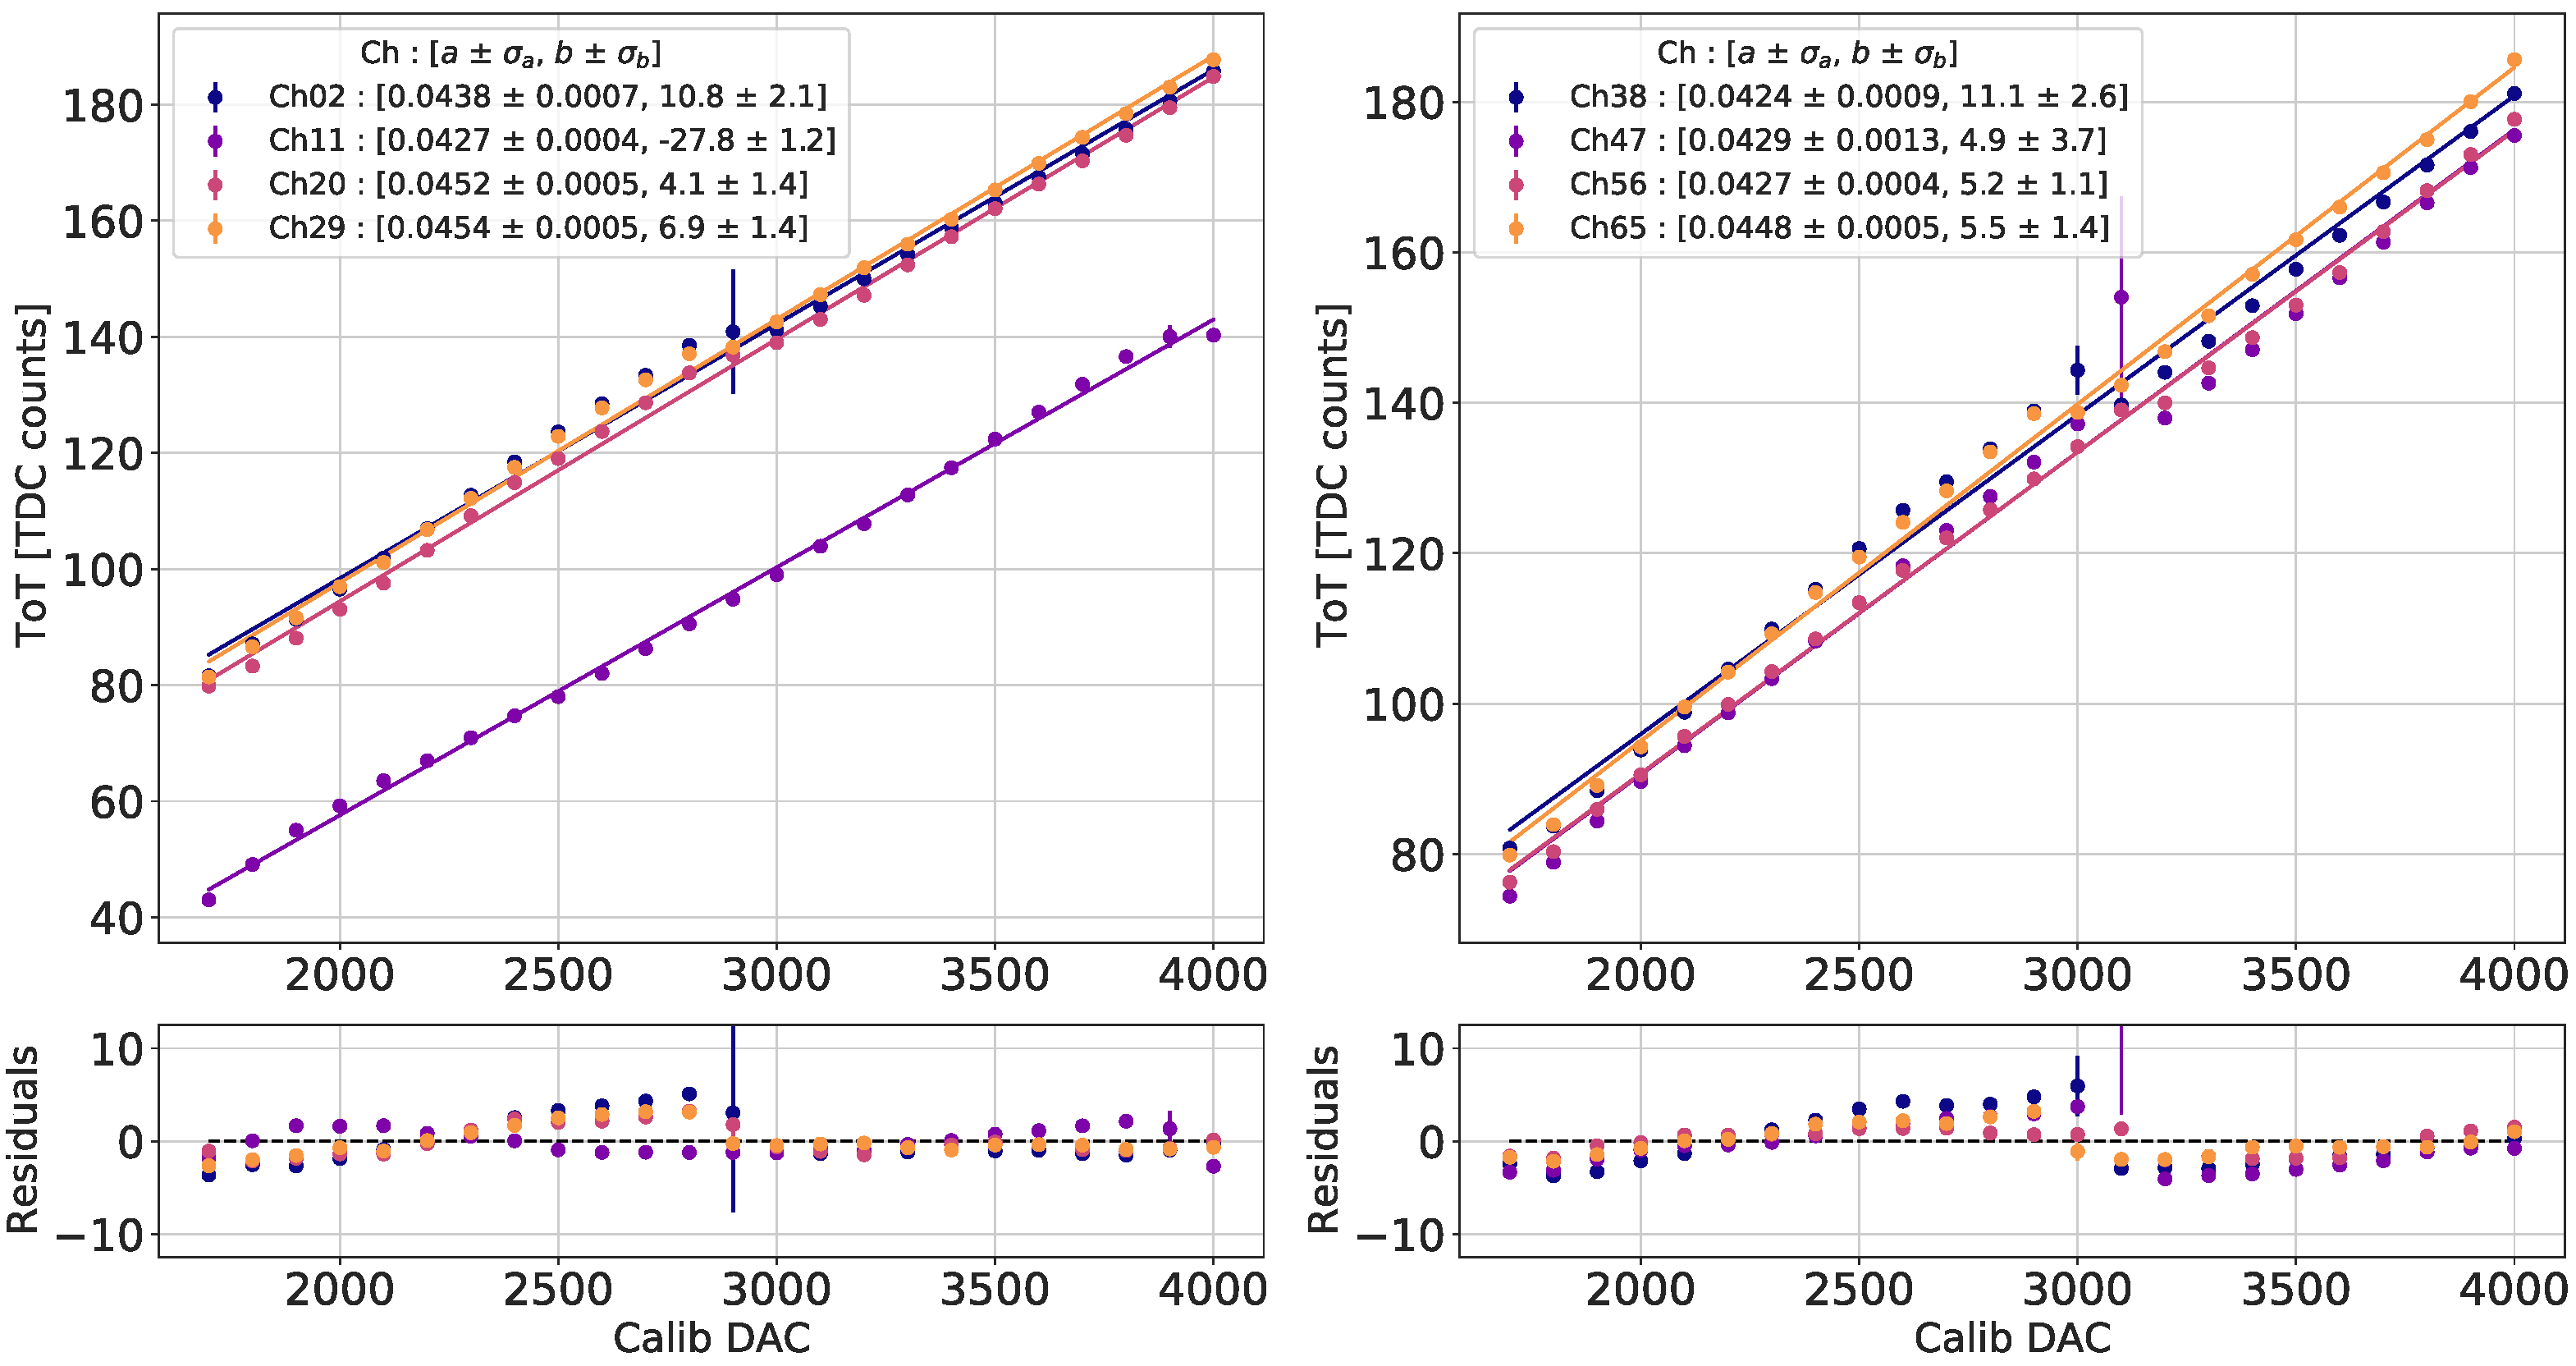
\includegraphics[width=0.75\linewidth]{Figures/HGCAL/TOT_Injection.pdf}
    \caption{The ToT response linearity to multiple injections corresponding to different \texttt{Calib\_DAC} values, defining the input charge. The  response is fitted with the linear function in Equation~\ref{eq:ADCLinearity} and the optimised parameters of the fit are reported in the legend.}
    \label{fig:TOT_Injection}
\end{figure}

When the preamplifier enters the saturation regime, the signal duration becomes proportional to the injected charge. Consequently, it is possible to estimate the signal amplitude through an indirect measurement of its saturation duration.

The Time-over-Threshold (ToT) technique measures the time difference between the start and the end of the saturation time. Figure~\ref{fig:TOT_Injection} illustrates the ToT measurements for different injected charges. The ToT curve is fitted by using Equation~\ref{eq:ADCLinearity} and the performance show a good linearity up to the highest charge of 500~fC. 

\subsubsection{The ToA performance}
\label{subsubsec:The ToA performance}

The time measurements are crucial to discriminate pile-up events and improve the particle identification in collision scenarios. This information is encoded in the Time-of-Arrival (ToA), corresponding to the time at which the signal amplitude exceeds the ToA threshold value.

The ToA measurement noticeably depends on the signal amplitude, since higher signals reach the discriminator threshold faster, while lower signals require more time to reach the threshold. This common behaviour is usually known as \textit{"time walk"} and needs to be considered as a correction when providing the time information.
Figure\ref{fig:TOA_Injection} clearly shows the time walk curve of the ToA measurement as a function of the signal amplitude. The time walk is parametrically described by Equation~~\ref{eq:TOATimeWalk} and the results for the fit parameters are reported for each channel in the legend.

\begin{equation}
    f(t) = \frac{a}{x-x_0}+b
\label{eq:TOATimeWalk}
\end{equation}

\bigbreak

For the HGCROC3 performance it is also interesting to evaluate the effect of the electronic noise on the time measurements. Amplitude variations due to electronic noise introduce an uncertainty on the timing of a signal crossing the defined threshold: the effect will be more accentuated for a low amplitude signal than for a high amplitude signal.

The \textit{"time jitter"} curve, describing the uncertainty on the timing measurement due to the electronic noise, is shown in Figure~\ref{fig:TOANoise_Injection}.
The trend can be described by Equation~\ref{eq:TOATimeJitter} and the parameters of the fit are reported in the legend of the plots.

\begin{equation}
    f(t) = \sqrt{\left(\frac{a}{x-x_0}\right)^2+b^2}
\label{eq:TOATimeJitter}
\end{equation}

\begin{figure}
    \centering
    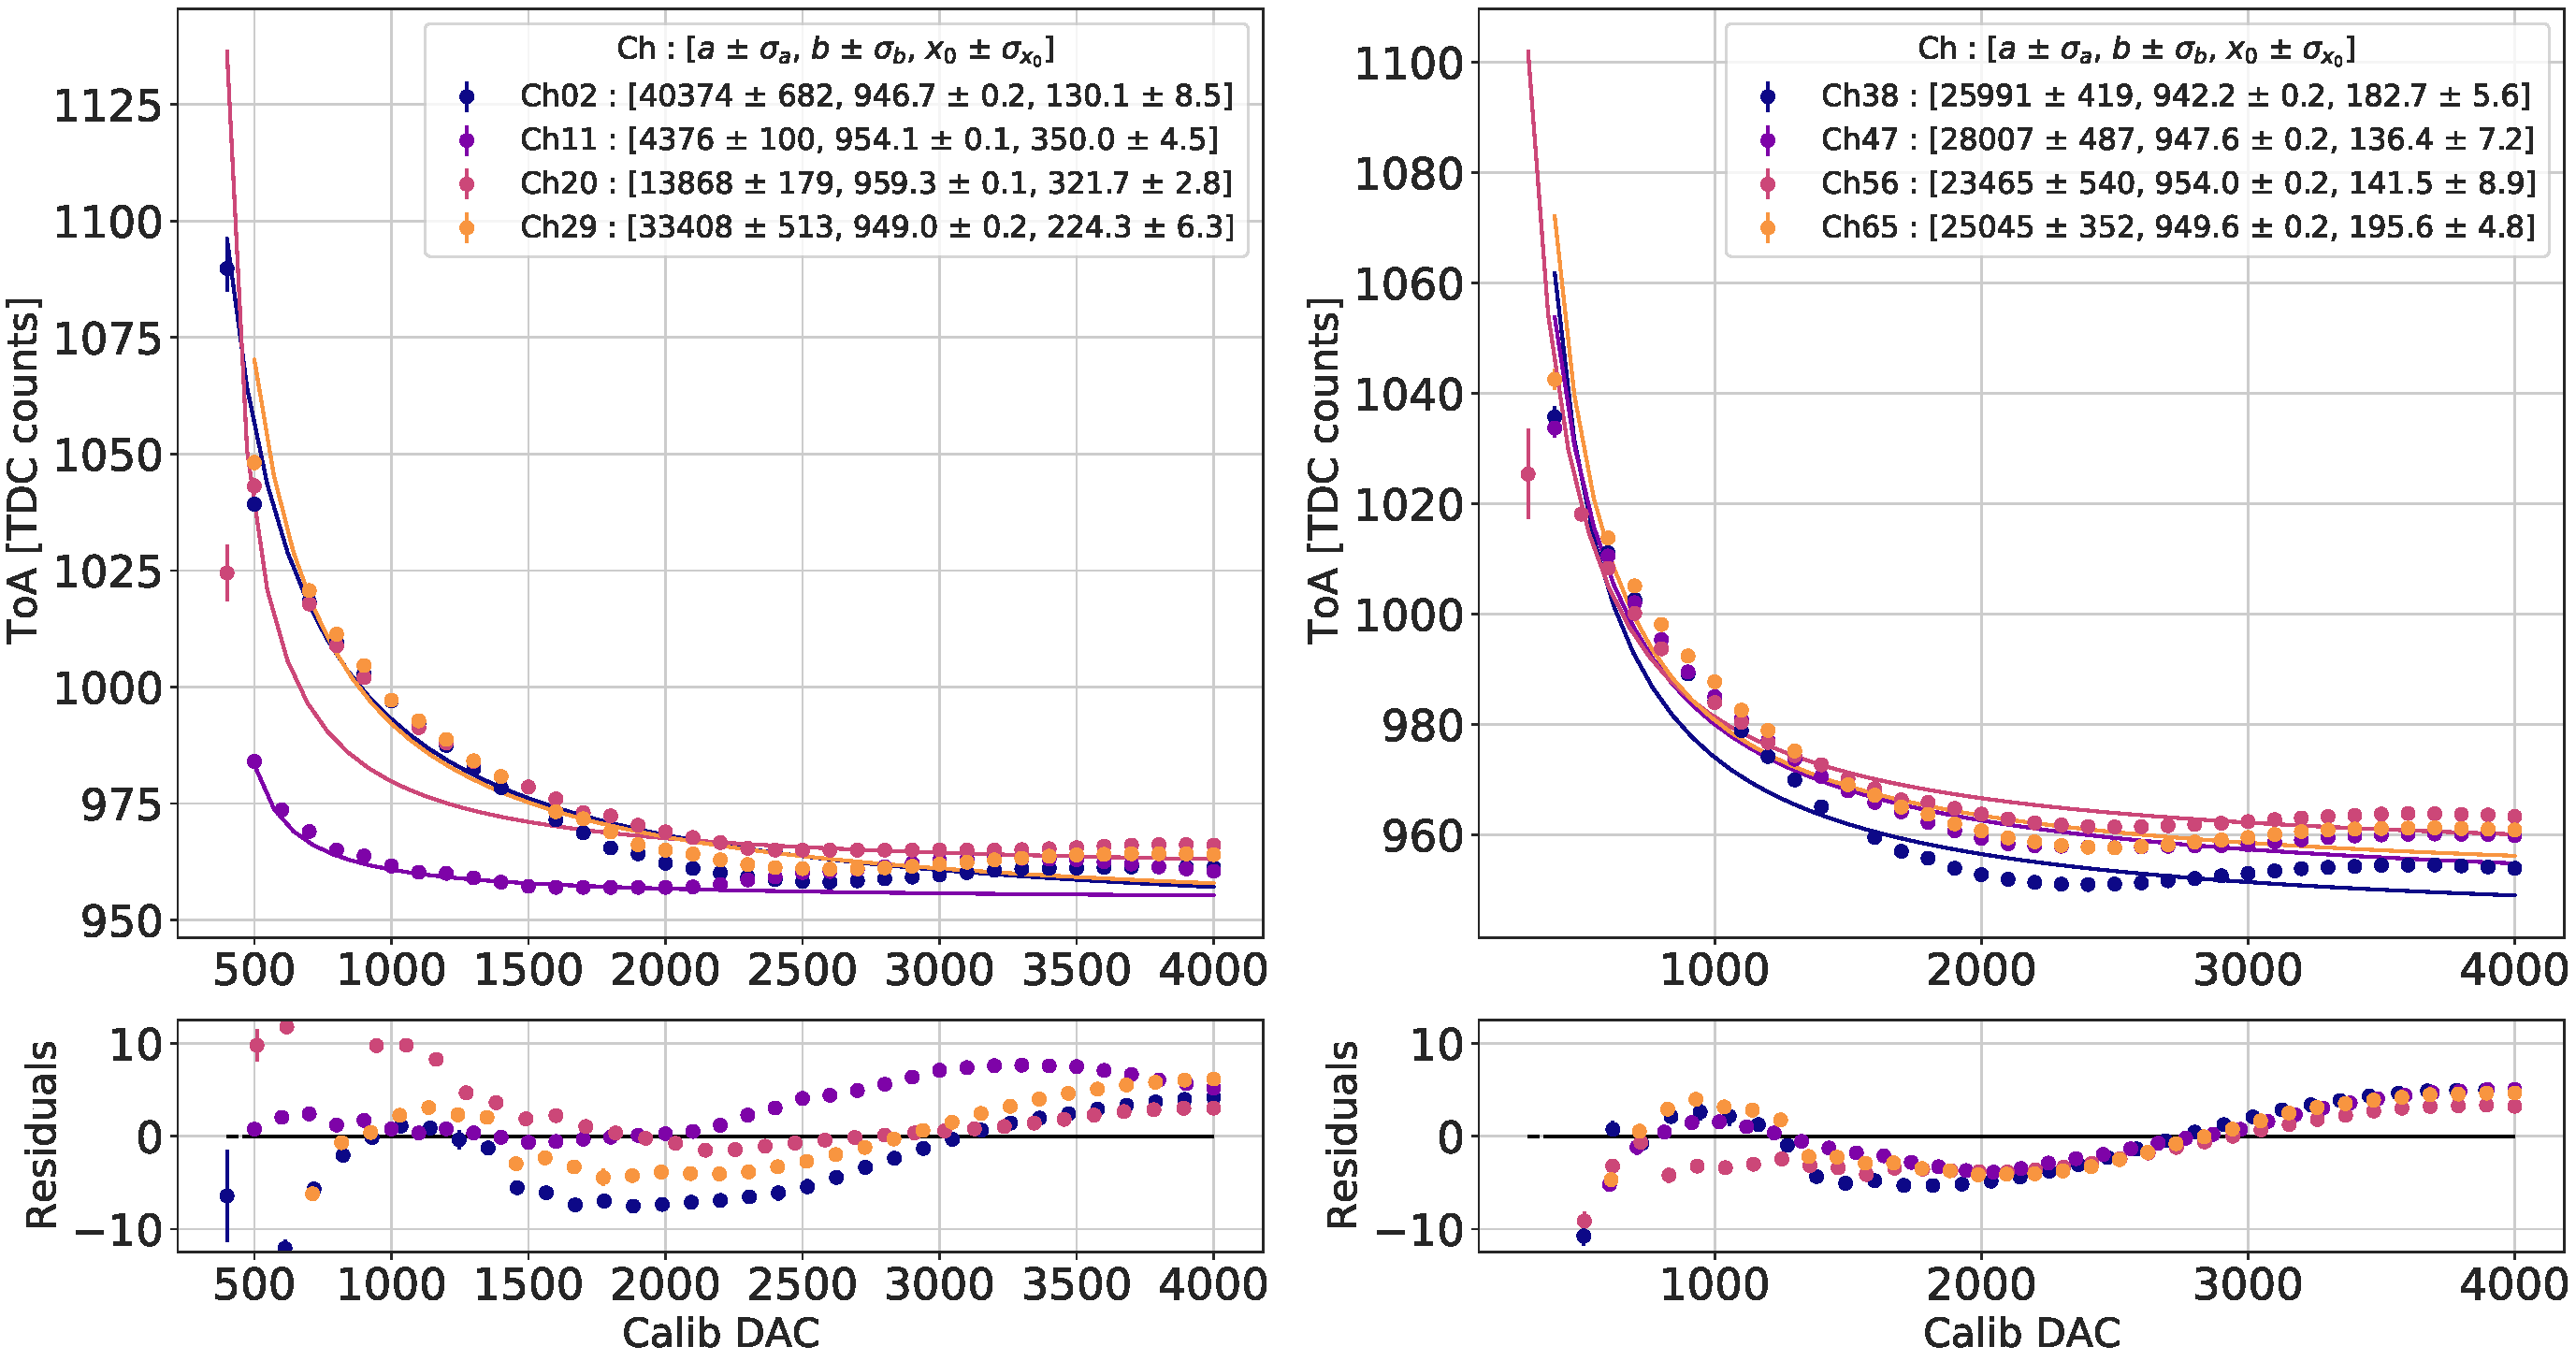
\includegraphics[width=0.75\linewidth]{Figures/HGCAL/TOA_Injection.pdf}
    \caption{The \textit{"time walk"} curve describing the ToA response to multiple injections corresponding to different \texttt{Calib\_DAC} values, defining the input charge. The  response is fitted with the function in Equation~\ref{eq:TOATimeWalk} and the optimised parameters of the fit are reported in the legend.}
    \label{fig:TOA_Injection}
\end{figure}

\begin{figure}
    \centering
    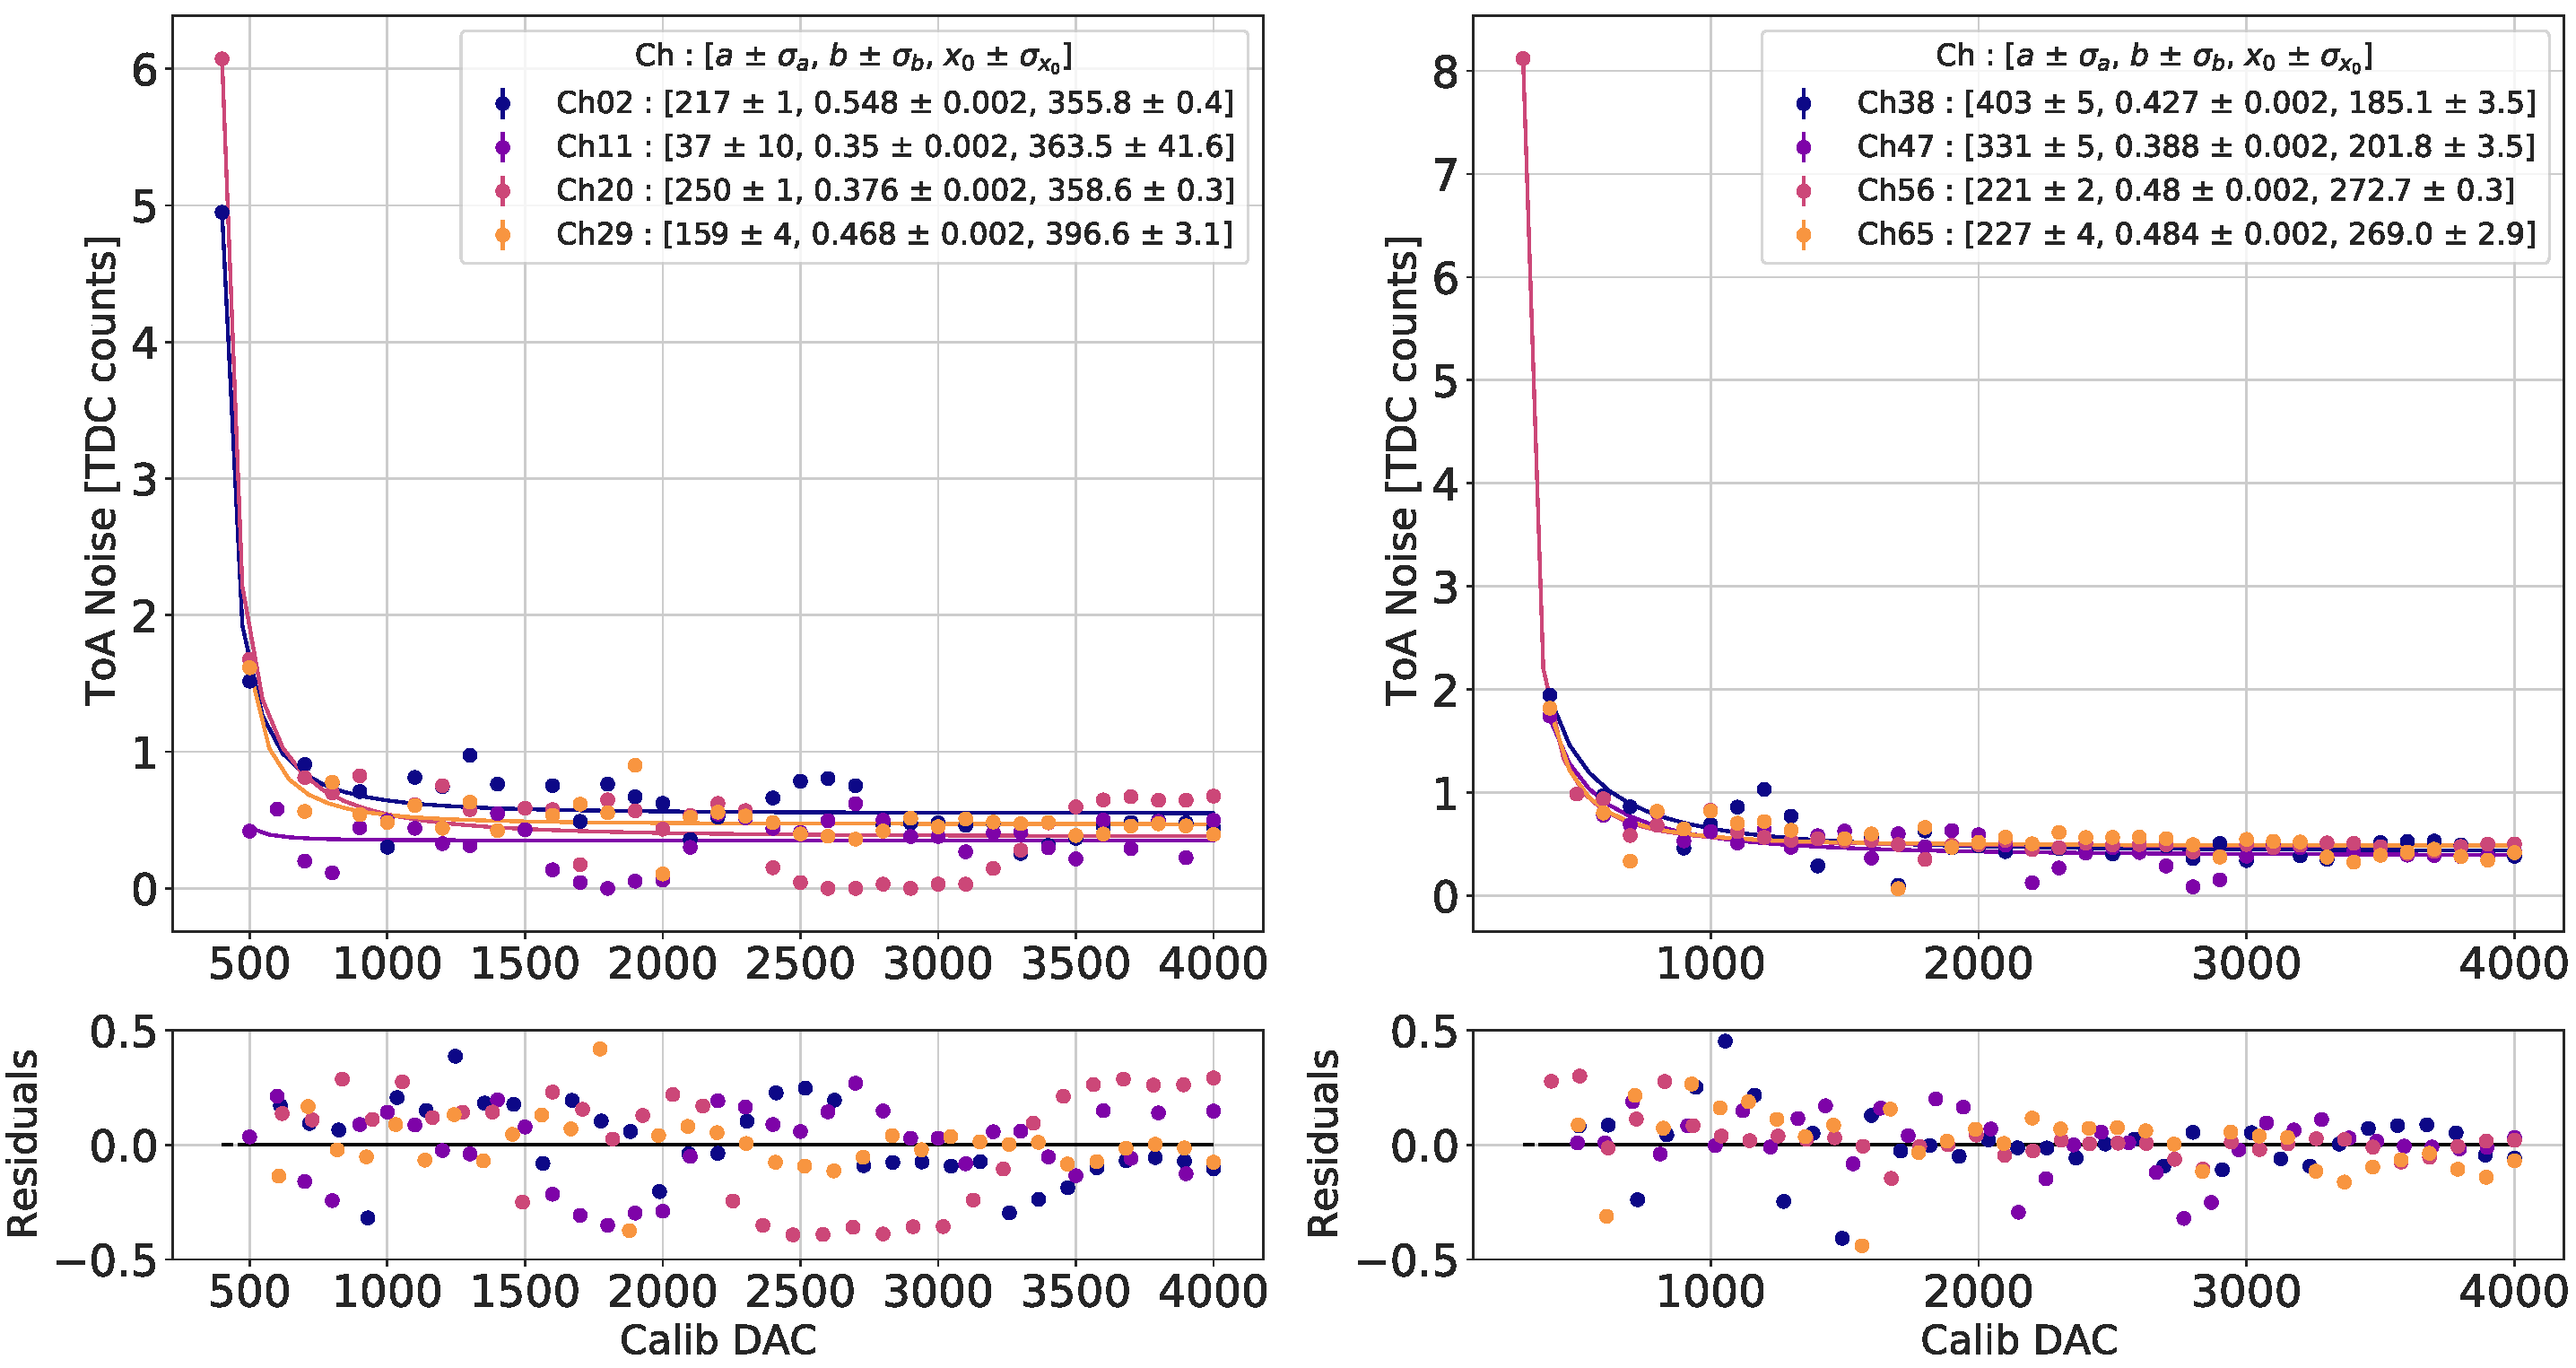
\includegraphics[width=0.75\linewidth]{Figures/HGCAL/ToANoise_Injection.pdf}
    \caption{The \textit{"time jitter"} curve describing the ToA noise to multiple injections corresponding to different \texttt{Calib\_DAC} values, defining the input charge. The  response is fitted with the function in Equation~\ref{eq:TOATimeJitter} and the optimised parameters of the fit are reported in the legend.}
    \label{fig:TOANoise_Injection}
\end{figure}

\subsection{The HGCROC3 batch testing}
\label{subsec:The HGCROC3 batch testing}

The HGCAL detector is expected to host approximately 120~K HGCROC3 read-out chips. The large number of ASICs poses significant challenges in both manufacturing and production, making it difficult to ensure each prototype meets its design specifications.

In order to guarantee high-quality standards for each HGCROC3 device, all the newly produced HGCROC3 chips will undergo a production testing, with the target of determining whether a given ASIC should be assembled on a hexaboard or should instead be rejected due to production defects or bad performance.

The production testing will be conducted at the Laboratorie Leprince-Ringuet and the Omega facility: it will take place as an automated process, carried out by a robotic arm able to move the chips to the testing location, where a series of tests will be performed. 
These tests will examine the main components and parameters of the chips to ensure they are correctly configurable, can communicate with the software interface, and meet expected performance.

\bigbreak

In order to gain statistics about the HGCROC3 performance and optimise the testing procedure, a preliminary batch testing has been conducted on 200 prototypes of HGCROC3. Since the robotic arm was still under development, the batch testing has been performed using the manual socket board, where the chip can be inserted by hand by means of a dedicated suction pen, as shown in Figure~\ref{fig:ManualSocket}.
The testing procedure is composed of an initial calibration, as described in Section~\ref{subsec:The calibration procedure}, and of a series of charge injections to assess the response of the device to different signal amplitudes in terms of ADC, ToA and ToT, as described in Section~\ref{subsec:The HGCROC3 performance}.

\bigbreak

The batch testing furnishes a good opportunity to tailor the testing procedure and the criteria to accept or reject the chips. At the same time, it allows one to collect enough statistics to spot recurring unexpected behaviours that might be linked to potential design issues.

The vast majority of the rejected chips, as expected, is due to the presence of non-connected channels, showing zero response due to manufacturing problems. 
However, other recurring unexpected behaviours in the chip performance have been observed, revealing design issues discussed in the following paragraphs. These issues have been thoroughly investigated to understand their causes and to find possible solutions to mitigate them.

\begin{figure}
    \centering
    \includegraphics[width=0.7\linewidth]{Figures/HGCAL/ManualSocket.pdf}
    \caption{Experimental set-up for the preliminary batch testing of the HGCROC3. The manual socket board supports the testing of several prototypes in series: the socket can be manually opened or closed to extract or insert the chip.}
    \label{fig:ManualSocket}
\end{figure}

\subsubsection{Issue in TDC initialisation}
\label{subsubsec:Issue in TDC initialisation}

The first issue found is related to incorrect initialization of the TDC component. This problem manifests as an entire half of the chip being unable to provide ToA and ToT information; however, the ADC component is not affected and shows good performance. The particularity of this issue lies in its random occurrence: the same device tested multiple times will randomly exhibit the issue or not. This behavior has been attributed to an incorrect initialization procedure of the TDC controller and can be fixed by simply changing the testing start-up sequence.
% Arounf 20 chips were showing the problem, but since it's not a chip-related problem, all of them could recover after testing the device multiple times.

\subsubsection{Issue in ADC conversion}
\label{subsubsec:Issue in ADC conversion}

\begin{figure}[b]
    \centering
    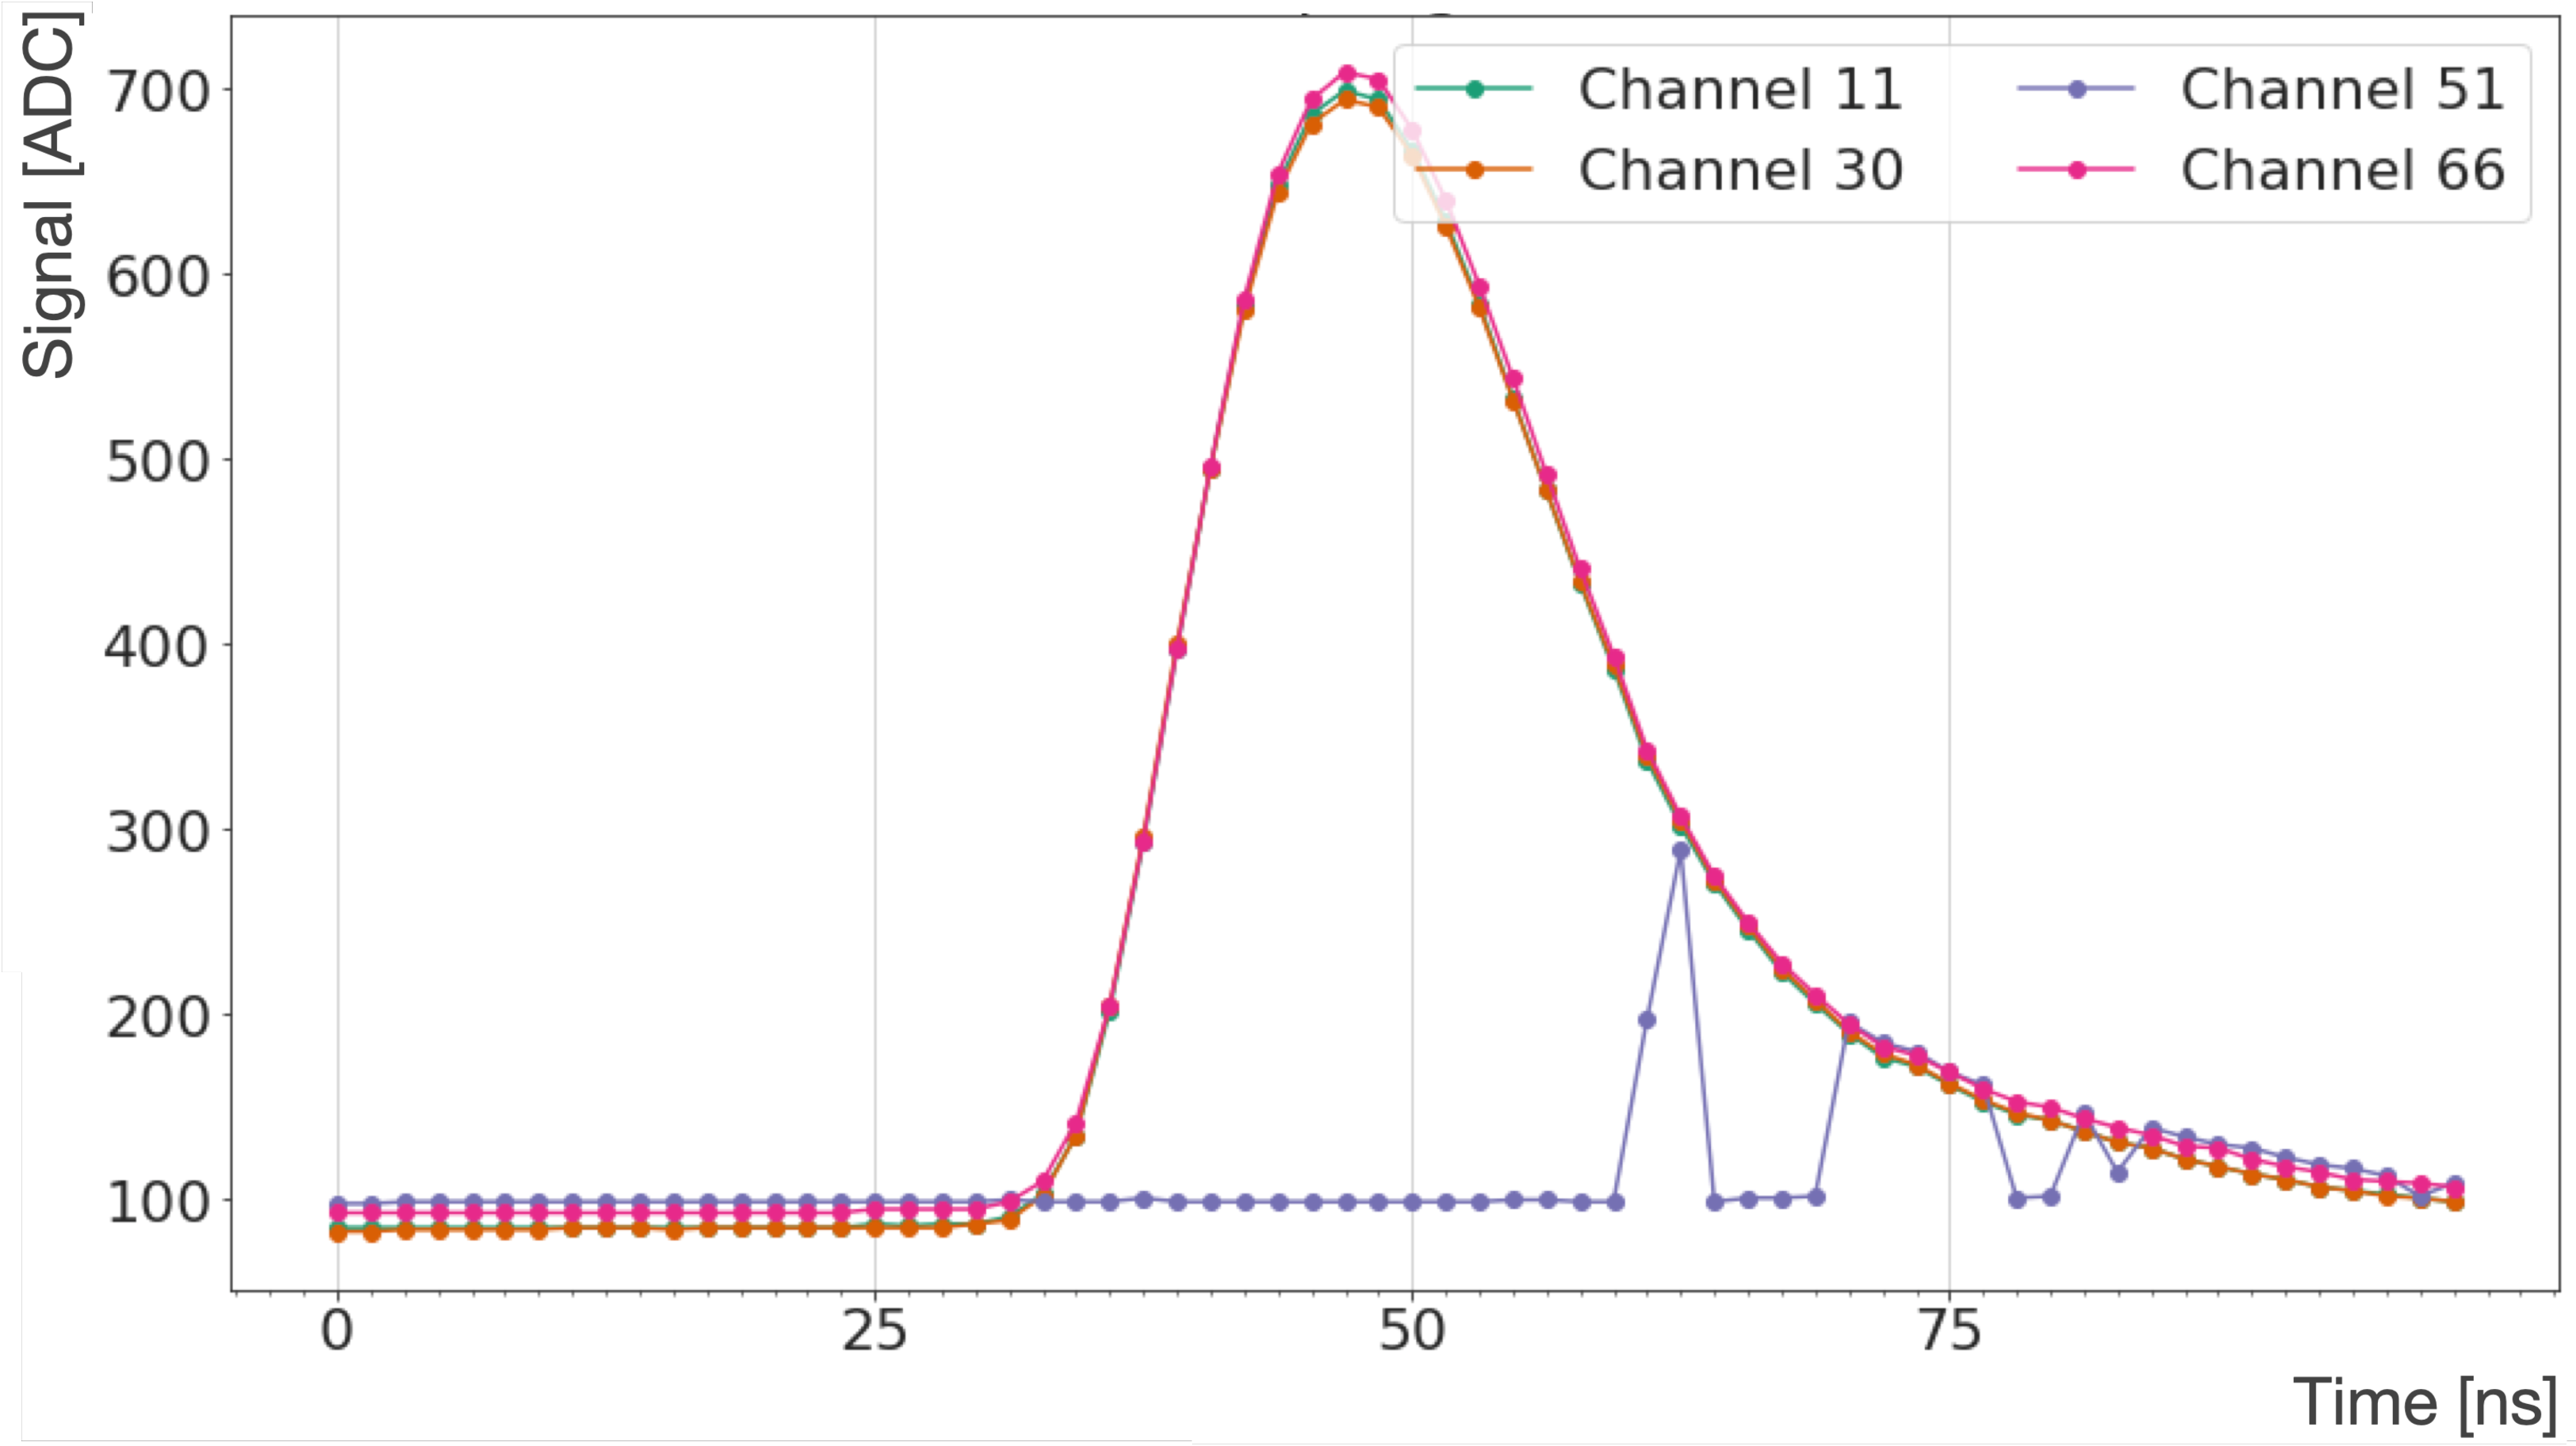
\includegraphics[height=0.25\linewidth]{Figures/HGCAL/ADCIssue_Median.pdf}
    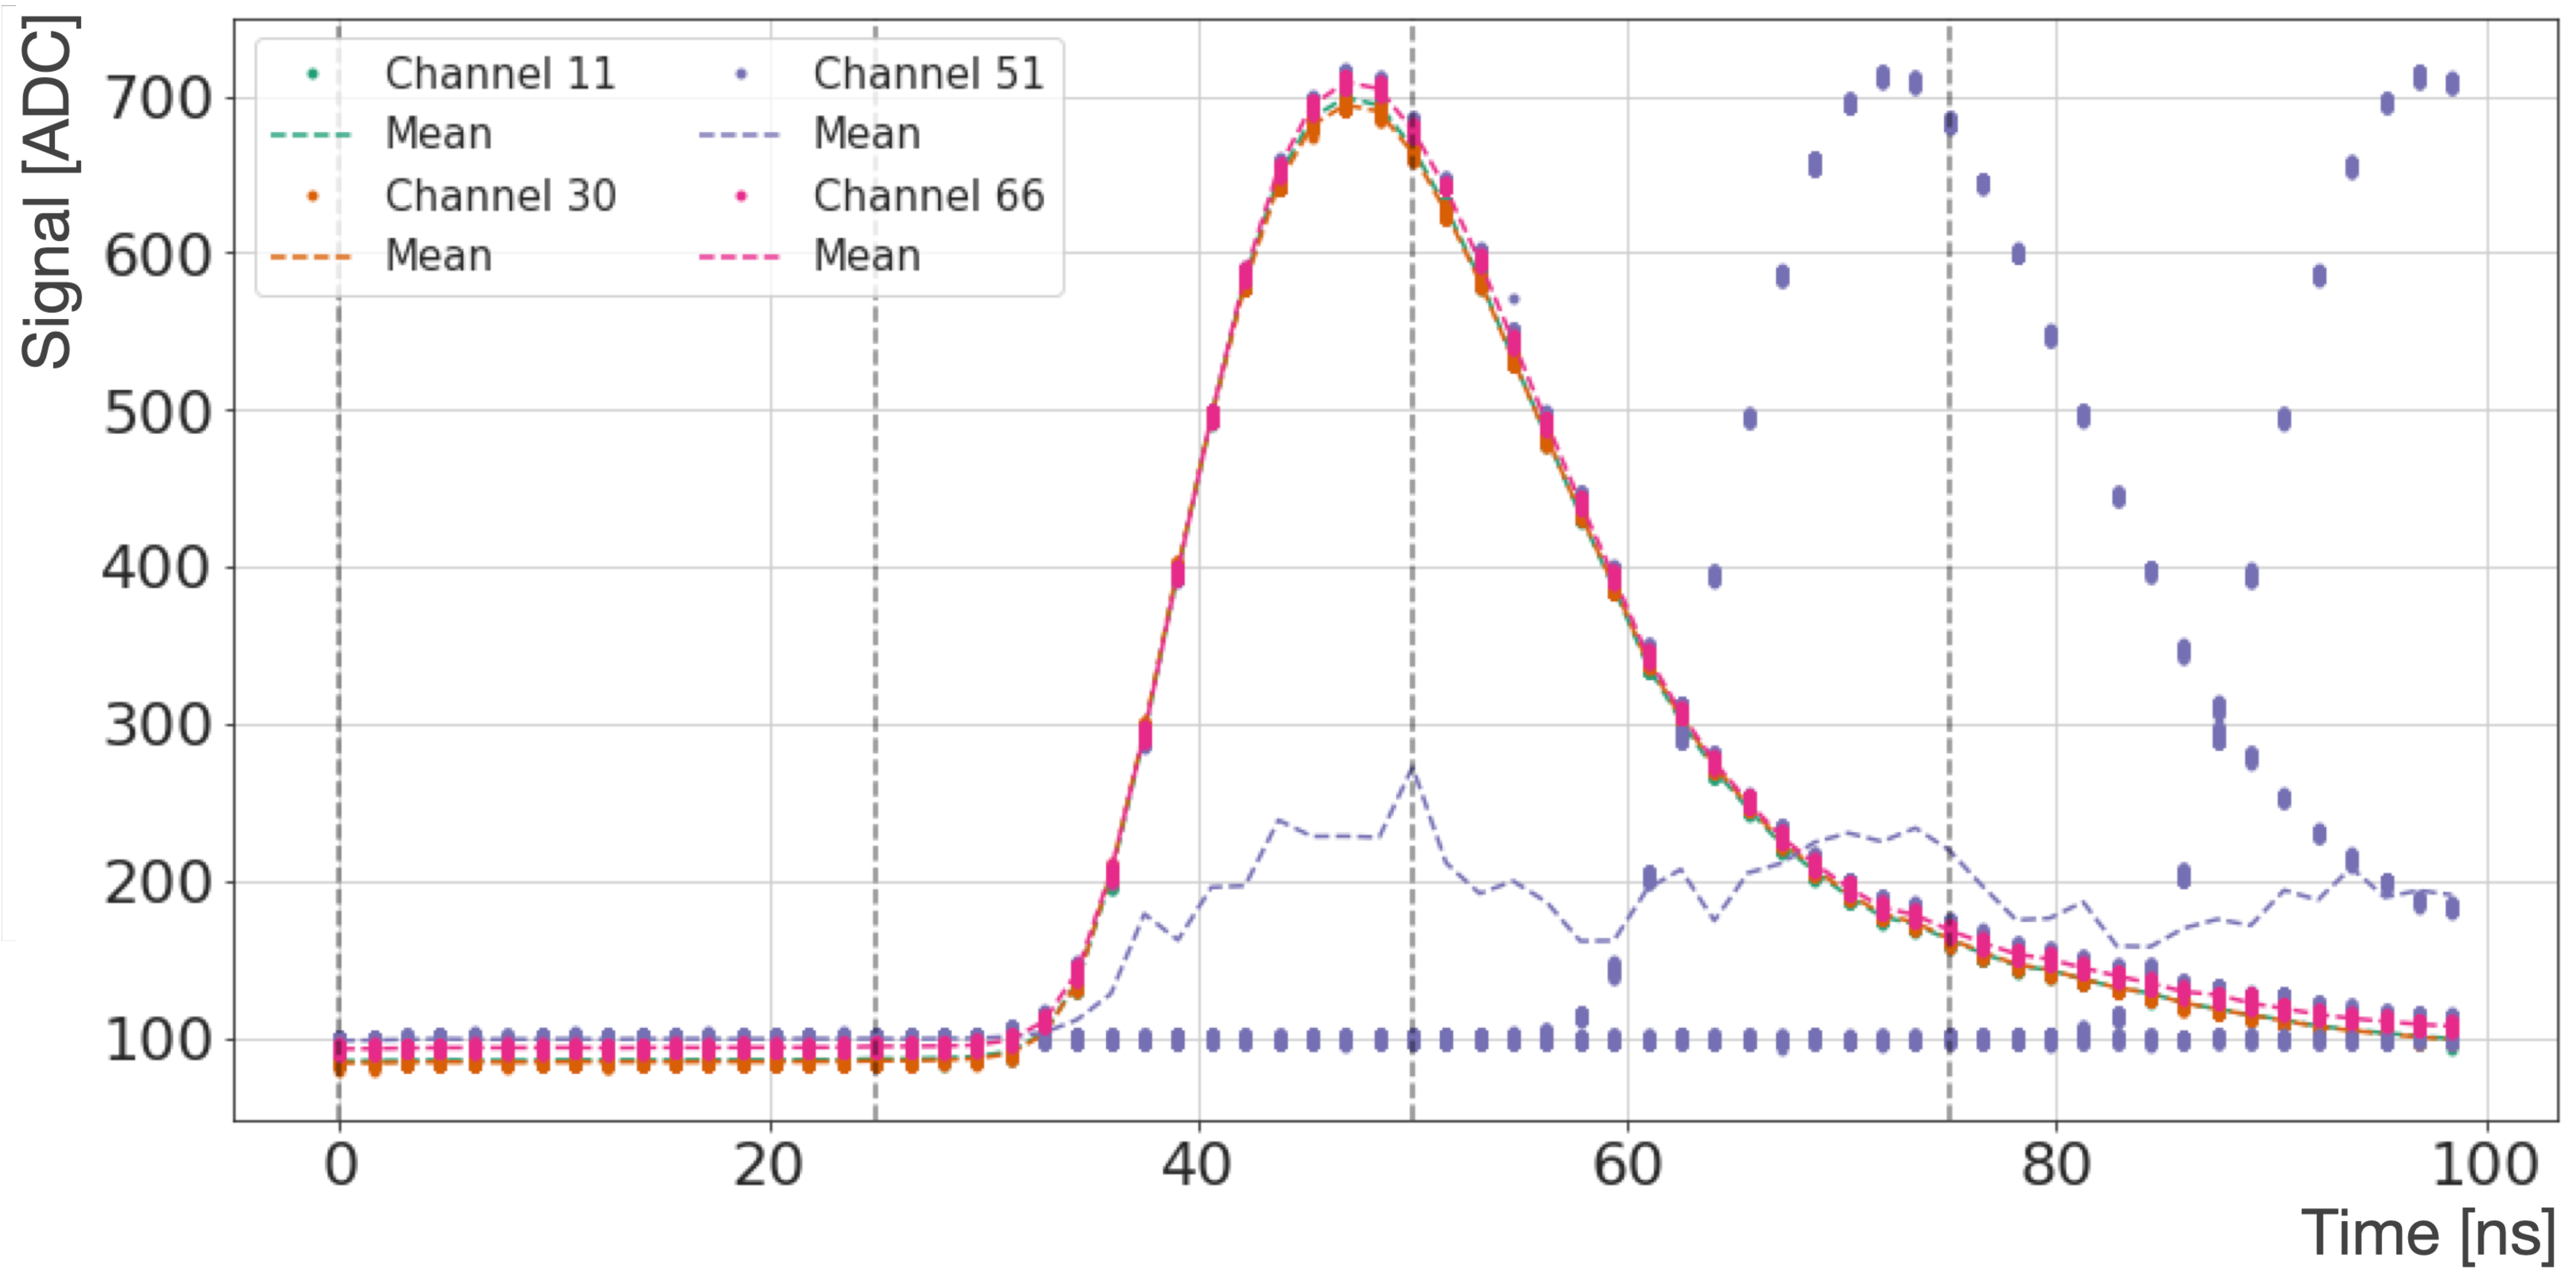
\includegraphics[height=0.25\linewidth]{Figures/HGCAL/ADCIssue_Raw.pdf}
    \caption{Example of data acquisition showing the issue in the ADC conversion: channels 11, 30, and 66 show the good expected performance, channel 51 shows unexpected behaviour. The left plot presents the previous testing procedure, reporting only the median value of multiple acquisitions. The right plot presents the updated testing procedure, revealing the signal reverberation caused by the ADC problem.}
    \label{fig:ADCIssue}
\end{figure}

The second issue is discovered in the ADC digitization process. The identification of this anomaly has proven challenging, due to the employed data acquisition techniques: each data point representing a signal pulse is given by the median value derived from multiple acquisitions (typically 100, though the number is configurable). This methodology is necessary to estimate the impact of the electron noise, which cannot be accurately assessed through a single injection.

With this data acquisition method, certain HGCROC3 prototypes exhibit inconsistent responses, confined to specific phases, as illustrated in the left plot of Figure~\ref{fig:ADCIssue}.

To elucidate the underlying cause of this behavior, individual injection events need to be examined. By analyzing each event separately, as depicted in the right plot of Figure~\ref{fig:ADCIssue}, it is possible to observe that certain events are inaccurately reconstructed in the wrong bunch crossing, leading to a signal reverberation shifted in time. The median value is anomalously influenced only during specific phases, depending on the number of misreconstructed events.

Since the existing testing method cannot detect the issue, the procedure is updated to represent all events independently. This revision reveals the presence of numerous channels afflicted by the same issue.

\bigbreak

Extensive investigations have been undertaken to determine the specific component responsible for this anomaly. Various tests have been executed to discern whether the issue was relates to the chip architecture or to external factors.

The analysis reveals that the anomaly exhibits dependency on both the conversion delay time and the operational temperature, as demonstrated in Figures~\ref{fig:ADCIssue_Delay} and ~\ref{fig:ADCIssue_Temperature}. However, even the minimum delay time and the reduced temperature of $-30^\circ$C fail to fully mitigate the issue across all channels, as each channel responded differently to delay and temperature changes. Given the significant impact of this issue on the chip performance, the ADC conversion circuit of the HGCROC3 has been revised, leading to the submission of an updated chip version to the manufacturers, which incorporated these corrections along with other necessary fixes.

\begin{figure}
    \centering
    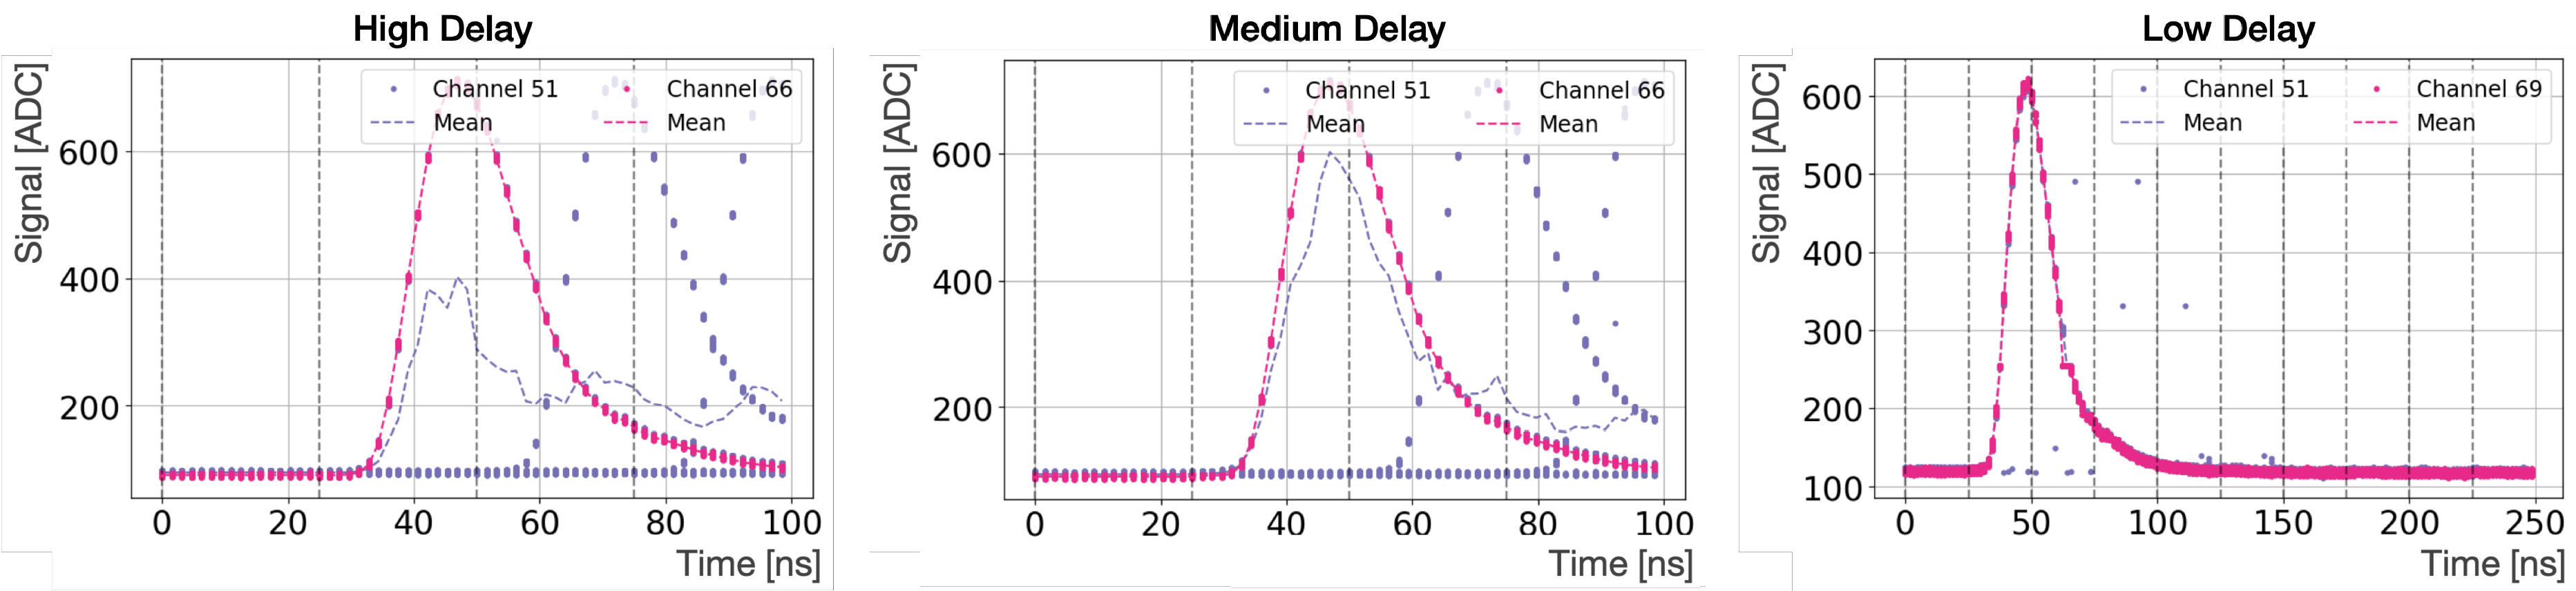
\includegraphics[width=0.99\linewidth]{Figures/HGCAL/ADCIssue_Delay.pdf}
    \caption{Dependency of the issue in the ADC conversion on the delay time for the conversion, configurable as a I2C parameter in the HGCROC3. The problematic channel 51 shows better performance for faster conversion times, but even the minimum delay time is not enough to entirely cancel the reverberation.}
    \label{fig:ADCIssue_Delay}
\end{figure}

\begin{figure}
    \centering
    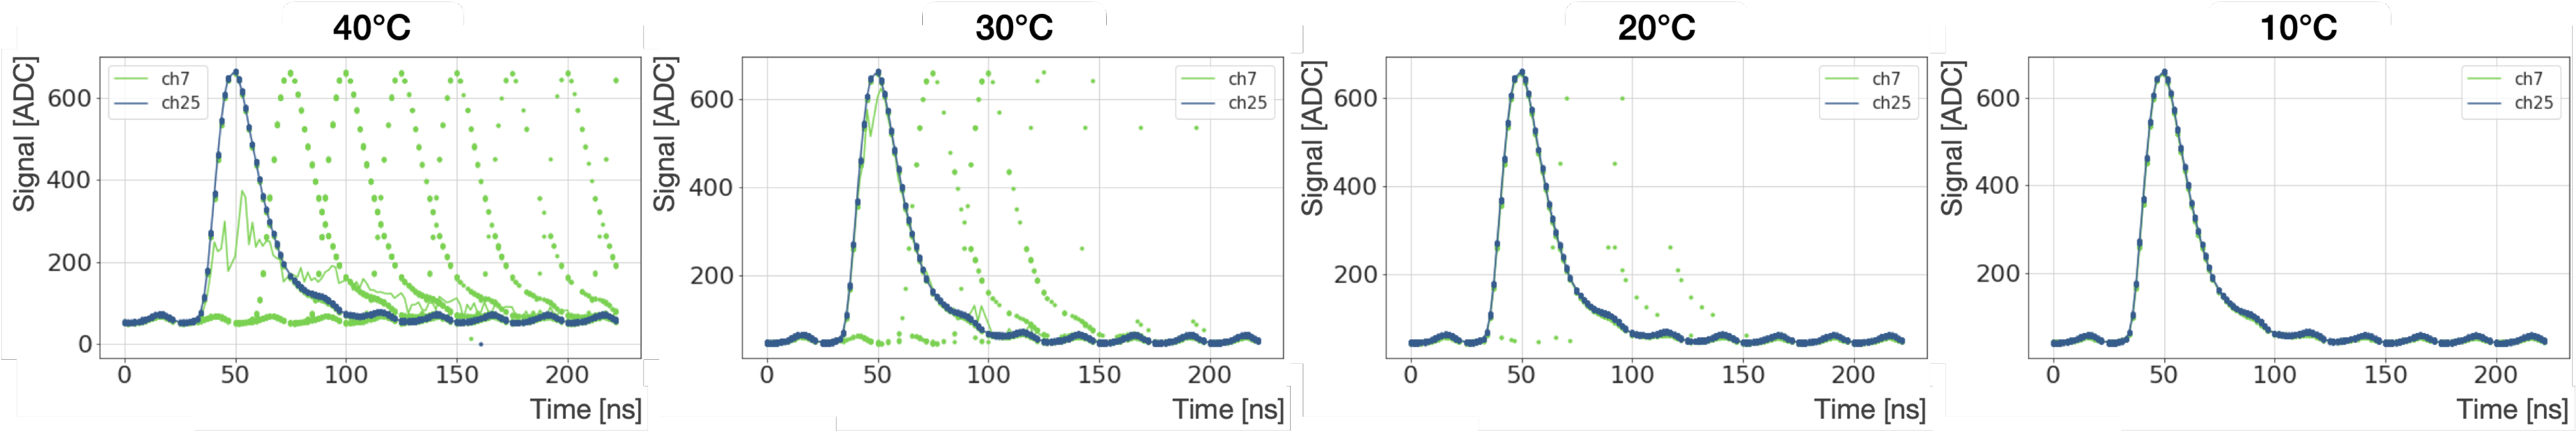
\includegraphics[width=0.99\linewidth]{Figures/HGCAL/ADCIssue_Temperature.pdf}
    \caption{Dependency of the issue in the ADC conversion on the temperature. The performance of the problematic channel 7 gradually improves with lower temperature and is completely restored when reaching $10^{\circ}$C.}
    \label{fig:ADCIssue_Temperature}
\end{figure}

\begin{figure}
    \centering
    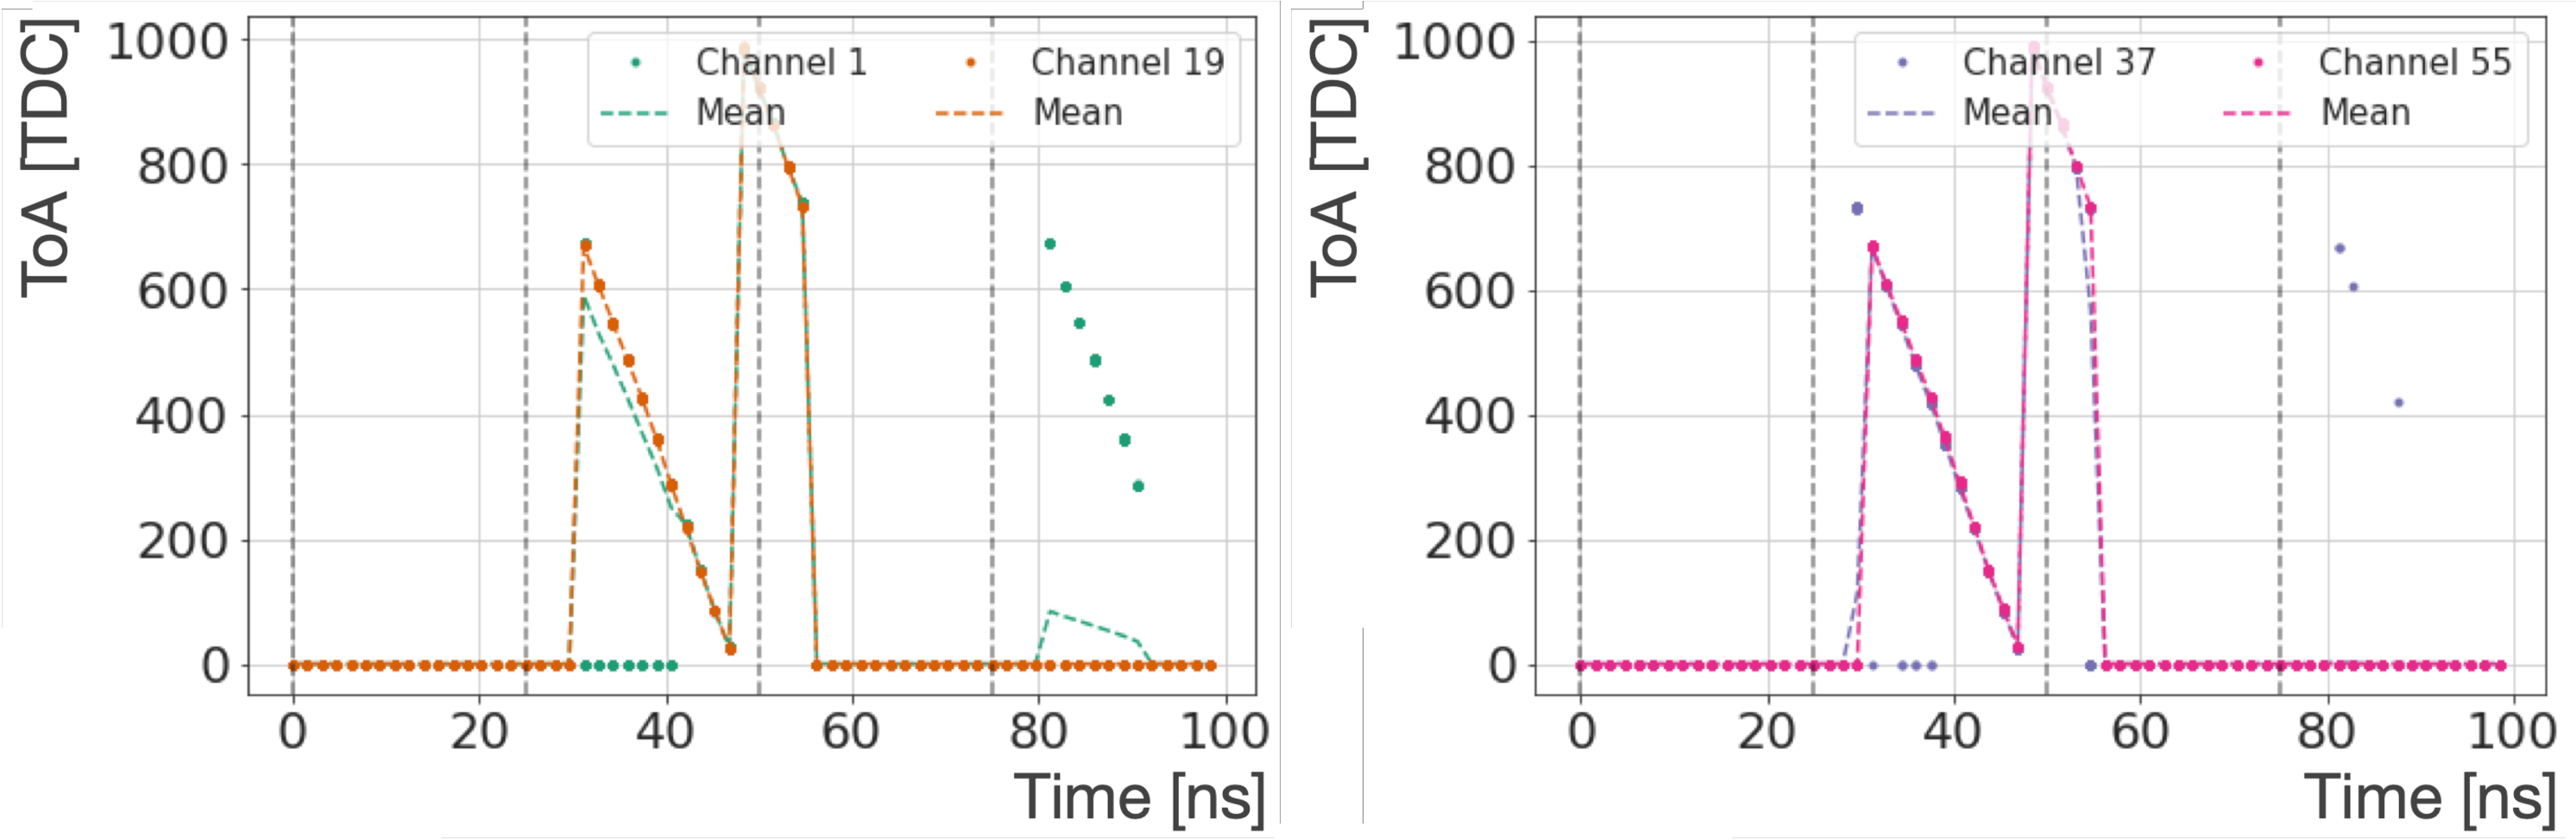
\includegraphics[width=0.8\linewidth]{Figures/HGCAL/TDCIssue.pdf}
    \caption{Example of data acquisition showing the issue in the TDC conversion: channels 19 and 55 show the good expected performance, channels 1 and 37 show unexpected behaviour, only visible by looking at the single events with the updated testing procedure.}
    \label{fig:TDCIssue}
\end{figure}

\subsubsection{Issue in TDC conversion}
\label{subsubsec:Issue in TDC conversion}

The new testing procedure has also led to the discovery of another issue in the conversion block of the TDC component, affecting the digitisation of the ToA and ToT values. 
An example of the anomalous behaviour is reported in Figure~\ref{fig:TDCIssue}. At a first glance, the manifestation appears analogous to that of the ADC conversion, with a reverberation of the signal in the incorrect bunch crossing period. However, a closer analysis reveals that the ToA measurement is correctly performed, but saved in the wrong bunch crossing. 

This behavior is linked to a metastability of the digitisation circuit in assigning the TDC information to the correct bunch crossing. This problem has been reproduced in the simulations and can be rectified through a slight modification of the TDC conversion circuit.

\bigbreak

A revised design of the chip allowed the ADC and TDC conversion problems to be fixed and has been implemented in the new version, HGCROC3b, which is the final chip design to be mounted on the HGCAL detector. 

%%%%%%%%%%%%%%%%%%%%%%%%%%%%%%%%%%%%%%%%%%%%%%%%%%%%%%%%%%%%%%%%%%%%%%%%%%%%%%%%%%%%%%%%%%%%
%%%%%%%%%%%%%%%%%%%%%%%%%%%%%%%%%%%%%%%%%%%%%%%%%%%%%%%%%%%%%%%%%%%%%%%%%%%%%%%%%%%%%%%%%%%%
%%%%%%%%%%%%%%%%%%%%%%%%%%%%%%%%%%%%%%%%%%%%%%%%%%%%%%%%%%%%%%%%%%%%%%%%%%%%%%%%%%%%%%%%%%%%
%%%%%%%%%%%%%%%%%%%%%%%%%%%%%%%%%%%%%%%%%%%%%%%%%%%%%%%%%%%%%%%%%%%%%%%%%%%%%%%%%%%%%%%%%%%%

\section{The HGCROC3 irradiation testing}
\label{sec:The HGCROC3 irradiation testing}

Once mounted on the HGCAL detector, the HGCROC3 will encounter the extremely harsh radiation environment of the CMS forward region. According to FLUKA \cite{fluka} simulations, the HGCAL front-end electronics will be subjected to a hadron flux up to $3.5\times10^6\,\textrm{s}^{-1}\,\textrm{cm}^{-2}$, with a total absorbed dose of approximately $200\,\textrm{Mrad}$ after the expected 10-year lifetime of the detector. 
The results of the FLUKA simulations, in terms of expected flux and integrated dose, are illustrated in Figure~\ref{fig:HGCALDose}. The high pseudorapidity regions of the detector, situated very close to the beam line, are predicted to experience the highest fluence, reaching up to $10^{16}\,\textrm{n}_{\textrm{eq}}\,\textrm{cm}^{-2}$.

\bigbreak

An essential step in the design validation of HGCROC3 is to test and quantify potential alterations in its performance under radiation exposure.
Radiation can severely impact electronics, causing memory errors, increased leakage currents, and in extreme cases, complete loss of functionality. These effects are a reliability concern not only in high-energy physics experiments, but also in long-term space missions, where devices endure prolonged exposure to Galactic Cosmic Radiation (GCR).

Radiation effects on electronic devices are traditionally categorised into two main categories:
\begin{itemize}
    \item [-] the Total Integrated Dose (TID) effects are a cumulative long-term degradation of the device due to prolonged exposure to ionizing radiation,
    \item [-] the Single Event Effects (SEE) are instantaneous device failures that can occur at any moment in a high-energy radiation environment, typically caused by direct interaction of particles with the device material.
\end{itemize}

The TID accumulated radiation damage typically impacts analog electronics more severely, with a lesser impact on digital memories or data processing components. After irradiation, a self-healing process known as \textit{annealing} can occur over time, gradually repairing these malfunctions.
In contrast, the SEE irradiation predominantly affects the digital part of the device, potentially leading to memory alterations and data transfer issues.

\begin{figure}
    \centering
    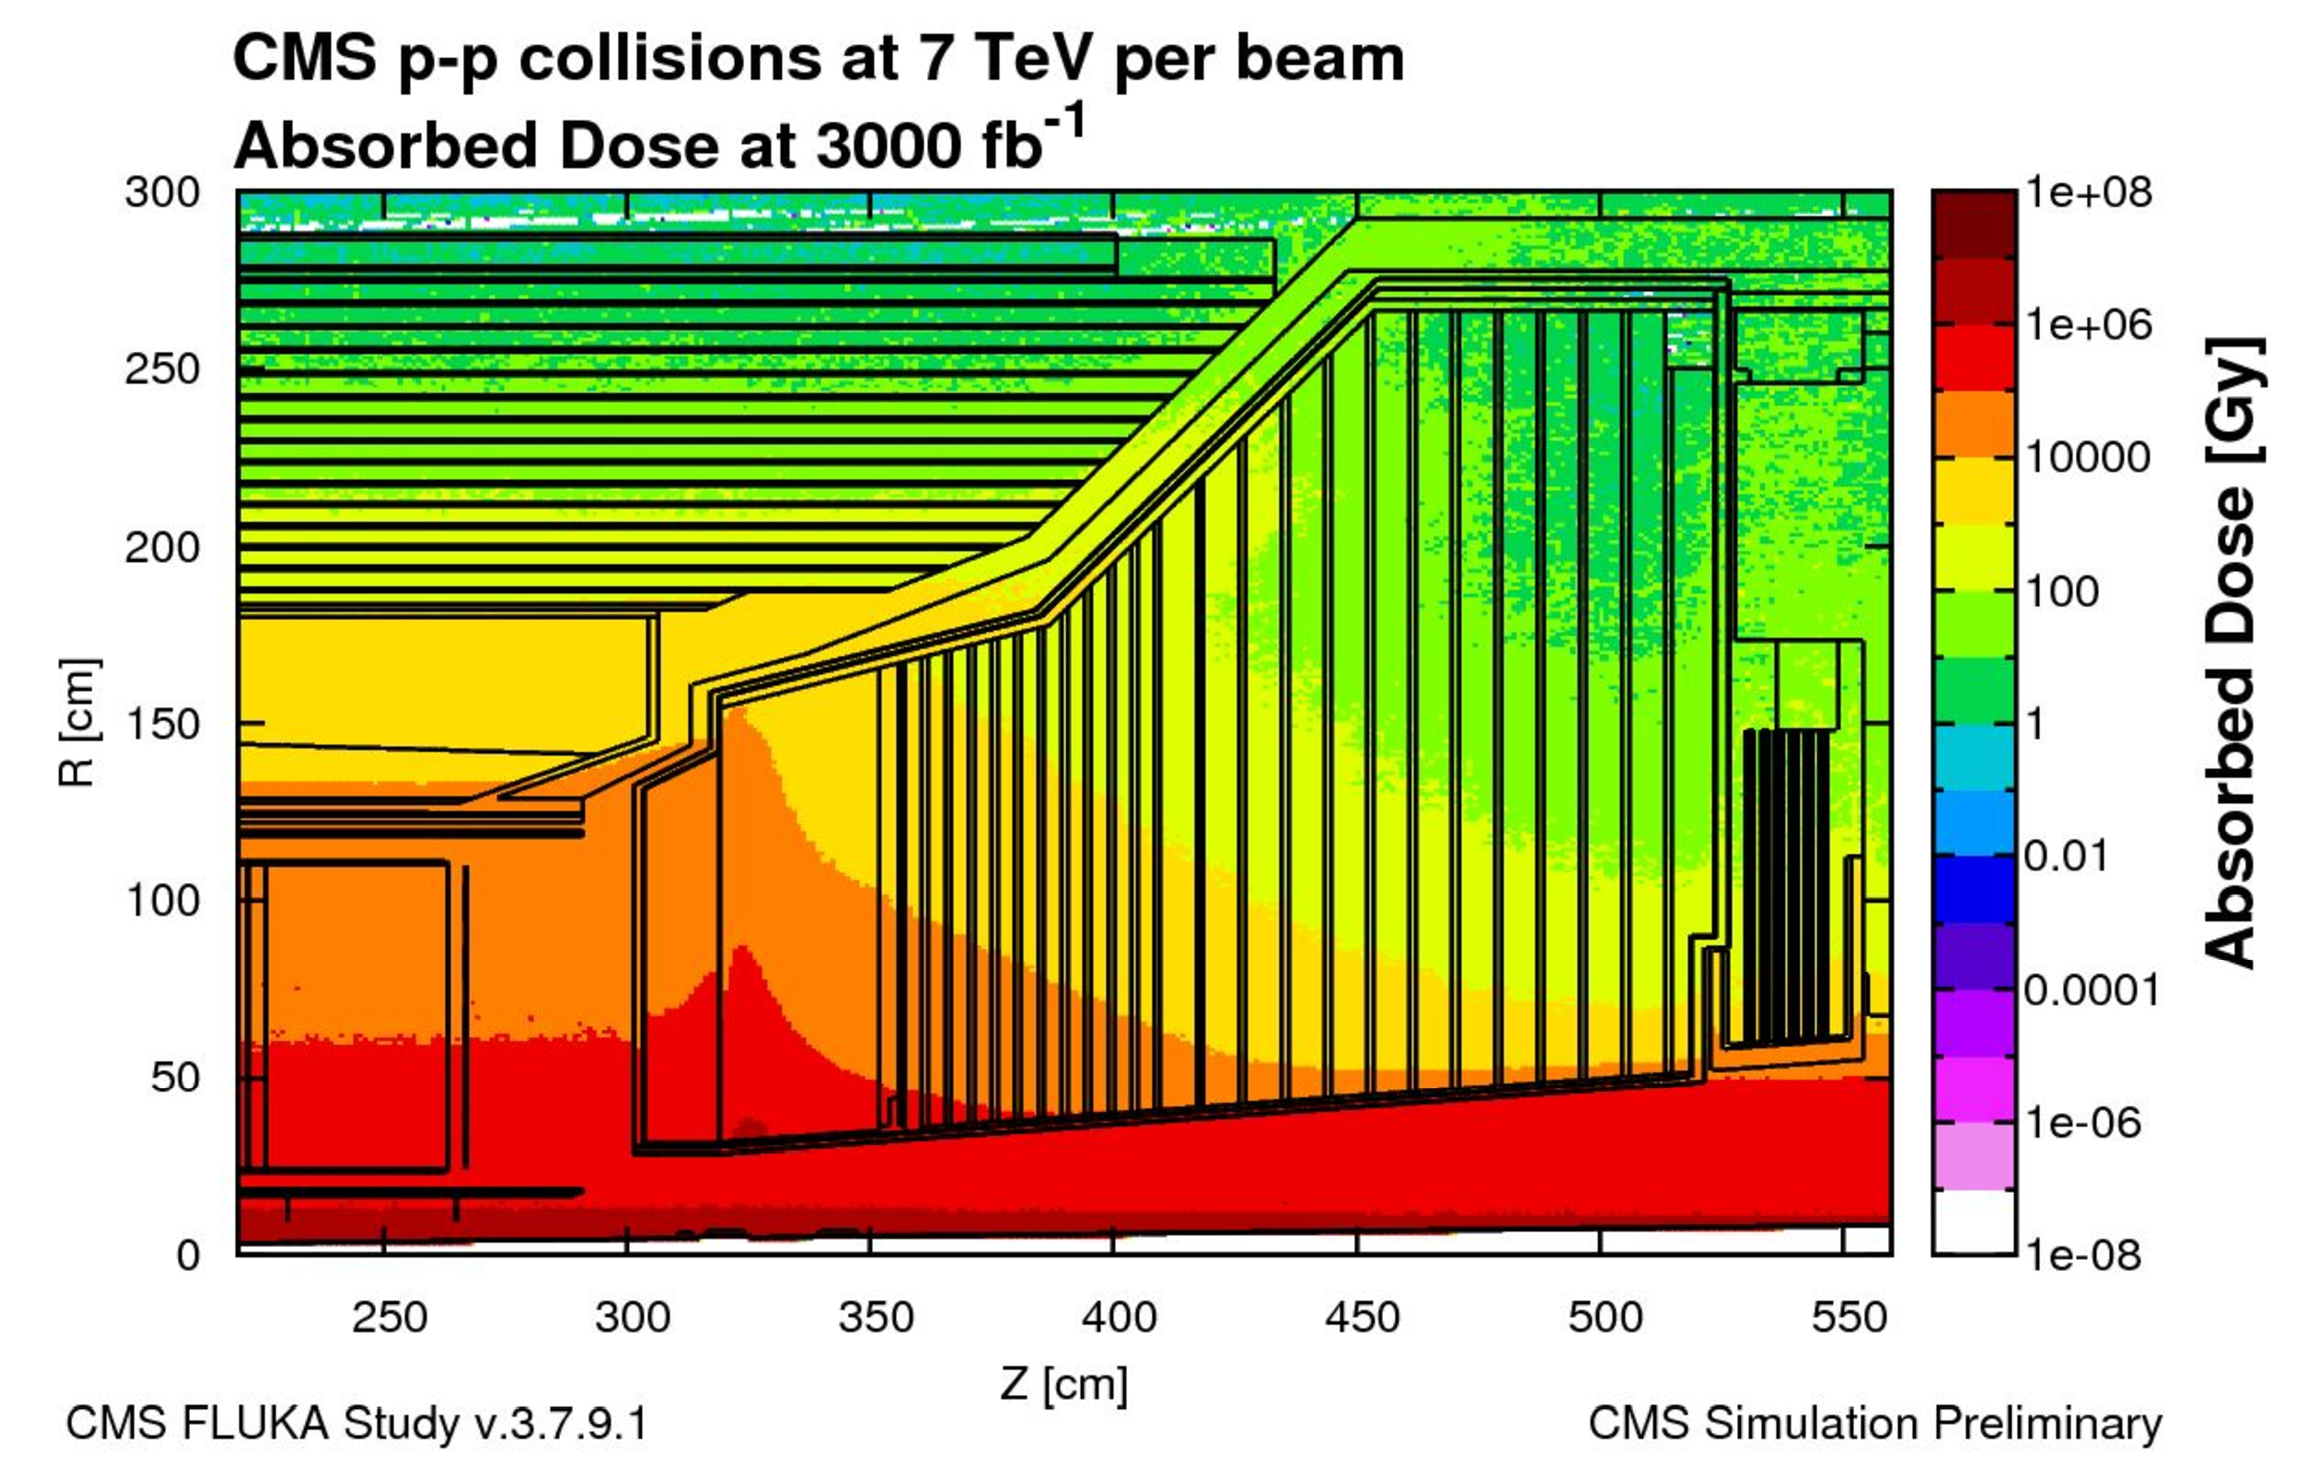
\includegraphics[width=0.49\linewidth]{Figures/HGCAL/HGCALDose.pdf}
    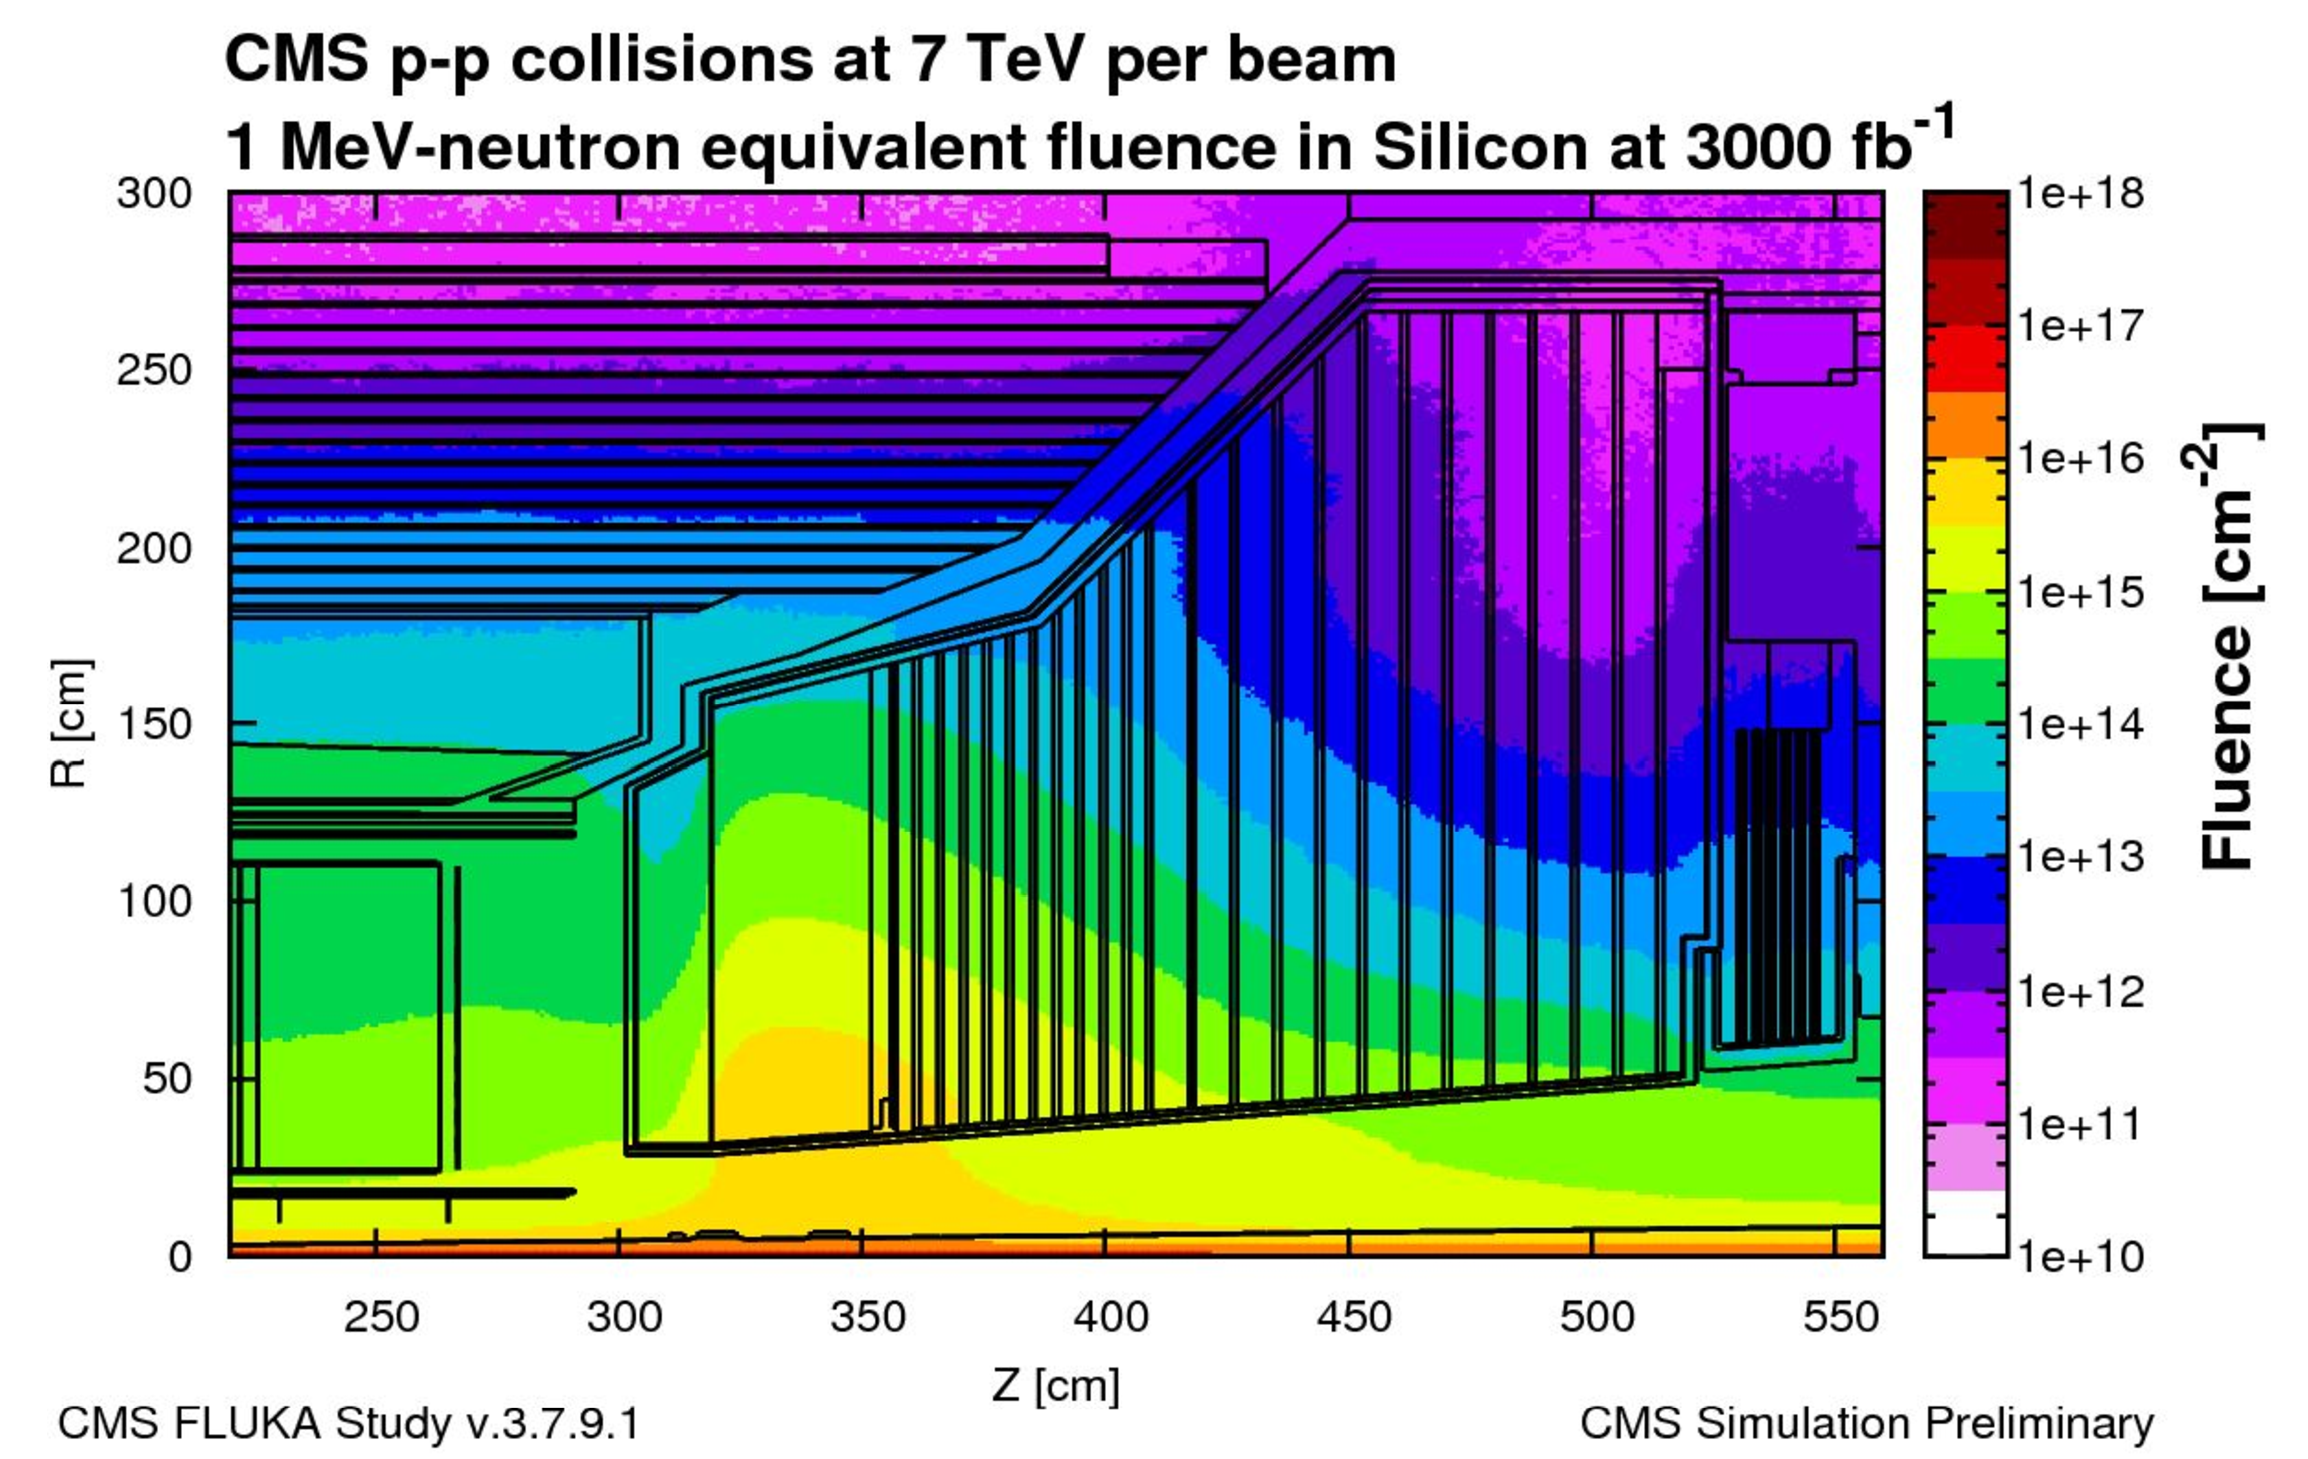
\includegraphics[width=0.49\linewidth]{Figures/HGCAL/HGCALFlux.pdf}
    \caption{Simulated dose (left) and fluence (right) of ionizing radiation accumulated in the HGCAL detector after an integrated luminosity of 3000 $\textrm{fb}^{-1}$, simulated using the FLUKA program, and shown as a two-dimensional map in the radial and longitudinal coordinates, $r$ and $z$.}
    \label{fig:HGCALDose}
\end{figure}

\bigbreak

The radiation hardness of modern electronic devices, particularly their resistance to both TID and SEE, is crucial for ensuring long-term reliability. The subsequent sections describe the irradiation campaigns conducted on the HGCROC3 to assess potential TID and SEE effects and to verify its radiation hardness.

%%%%%%%%%%%%%%%%%%%%%%%%%%%%%%%%%%%%%%%%%%%%%%%%%%%%%%%%%%%%%%%%%%%%%%%%%%%%%%%%%%%%%%%%%%%%
%%%%%%%%%%%%%%%%%%%%%%%%%%%%%%%%%%%%%%%%%%%%%%%%%%%%%%%%%%%%%%%%%%%%%%%%%%%%%%%%%%%%%%%%%%%%
%%%%%%%%%%%%%%%%%%%%%%%%%%%%%%%%%%%%%%%%%%%%%%%%%%%%%%%%%%%%%%%%%%%%%%%%%%%%%%%%%%%%%%%%%%%%
%%%%%%%%%%%%%%%%%%%%%%%%%%%%%%%%%%%%%%%%%%%%%%%%%%%%%%%%%%%%%%%%%%%%%%%%%%%%%%%%%%%%%%%%%%%%

\subsection{Total Integrated Dose}
\label{subsec:Total Integrated Dose} 

The Total Integrated Dose (TID) irradiation test aims at evaluating the cumulative radiation damage induced by ionizing particles on the HGCROC3 and at proving its radiation tolerance up to $200\,\textrm{Mrad}$. By reproducing the long-term effects of radiation exposure, the TID test identifies potential vulnerabilities in the device design and functionality.

\bigbreak

The first TID campaign on the HGCROC3 is performed at the Obelix facility (CERN) using a 10~keV X-ray beam. The experimental set-up is illustrated in Figure~\ref{fig:TID_Setup}.
The X-ray machine is placed inside a chamber for both radiation shielding and better humidity control, to prevent condensation when operating the electronics at temperatures below $0^{\circ}$C. 
The prototype of the HGCROC3 is mounted on a mezzanine board and thinned from its original thickness of $250\,\mu\textrm{m}$ to $70\,\mu\textrm{m}$, for a better X-ray penetration.
The cooling system is configured with a copper plaque adhering to the mezzanine board, and two resistive sensors are placed close to the device to monitor temperature stability.

\bigbreak

Studies have shown that the radiation damage caused by ionizing particles is dependent on both temperature and dose rate~\cite{giulio}.
\begin{itemize}
    \item [-] Irradiation has a more significant impact at higher temperatures.  Ideally, the TID irradiation test should be performed at the expected HGCAL operating temperature of $-30^{\circ}$C; however such a low temperature is hardly reached by the available experimental set-up, consequently this campaign provides a worst-case scenario. 
    \item [-]  Additional radiation damage can arise at low dose rates. However, reaching the final dose of $200\,\textrm{Mrad}$ with the expected HL-LHC dose rate of $\sim10^2,\textrm{rad/h}$ would be hardly reproducible with a testing campaign. For this reason, a margin of at least +$50\%$ on the total injected dose should be considered during the irradiation testing at higher dose rates to account for this difference. 
\end{itemize}

During the HGCROC3 TID irradiation campaign, the chip is operated at $-10^{\circ}$C, the minimum temperature available for the experimental set-up, and the dose rate is set to the highest possible value of $2.45\,\textrm{Mrad/h}$, in order to complete the test within the available one-week time frame. 
To account for the different dose rate with respect to the HL-LHC conditions, a +$75\%$ margin is considered in addition the the total expected dose of $200\,\textrm{Mrad}$.
At the end of the TID radiation exposure, the total integrated dose delivered to the HGCROC3 is $345\,\textrm{Mrad}$.

\bigbreak

During the exposure time, the performance of the HGCROC3 is continuous monitored in terms of power consumption, ADC and TDC measurements. The results are described in the following paragraphs. 

\begin{figure}
    \centering
    \includegraphics[height=0.32\linewidth]{Figures/HGCAL/TID_Setup1.pdf}
    \includegraphics[height=0.32\linewidth]{Figures/HGCAL/TID_Setup2.pdf}
    \caption{The experimental set-up for the TID irradiation campaign performed at the Obelix facility (CERN). On the left, a picture of the X-ray machine, located above the mezzanine board hosting the HGCROC3 prototype; the FPGA board is located away from the X-ray beam to protect it from radiation damage. On the right, a close-up on the mezzanine board hosting the HGCROC3, tightly fixed through a white plastic support to the cooling system plaque underneath; the copper tubes connected to the cooling system and the resistive temperature sensors are also visible.}
    \label{fig:TID_Setup}
\end{figure}

\subsubsection{ADC and TDC performance}
\label{subsubsec:ADC and TDC performance}

During the TID radiation exposure, no impact on the charge or time measurements and no misbehaviour in the DRAMs is observed. The ADC and TDC performance against injected charge after irradiation remains consistent with pre-irradiation conditions.
Figure~\ref{fig:TID_SignalShape} and Figure~\ref{fig:TID_ADCLinearity} show the comparison of the ADC performance before and after the radiation exposure: the recorded signal shape does not show any degradation, and the the rising and falling edge time constants are unaffected. Additionally, the recorded signal amplitude maintains the expected linear dependency on the injected input charge.
Figure~\ref{fig:TID_TimeWalk} presents the comparison of the TDC performance on the ToA measurement before and after radiation exposure, showing no degradation in the TDC component performance.

\begin{figure}
    \centering
    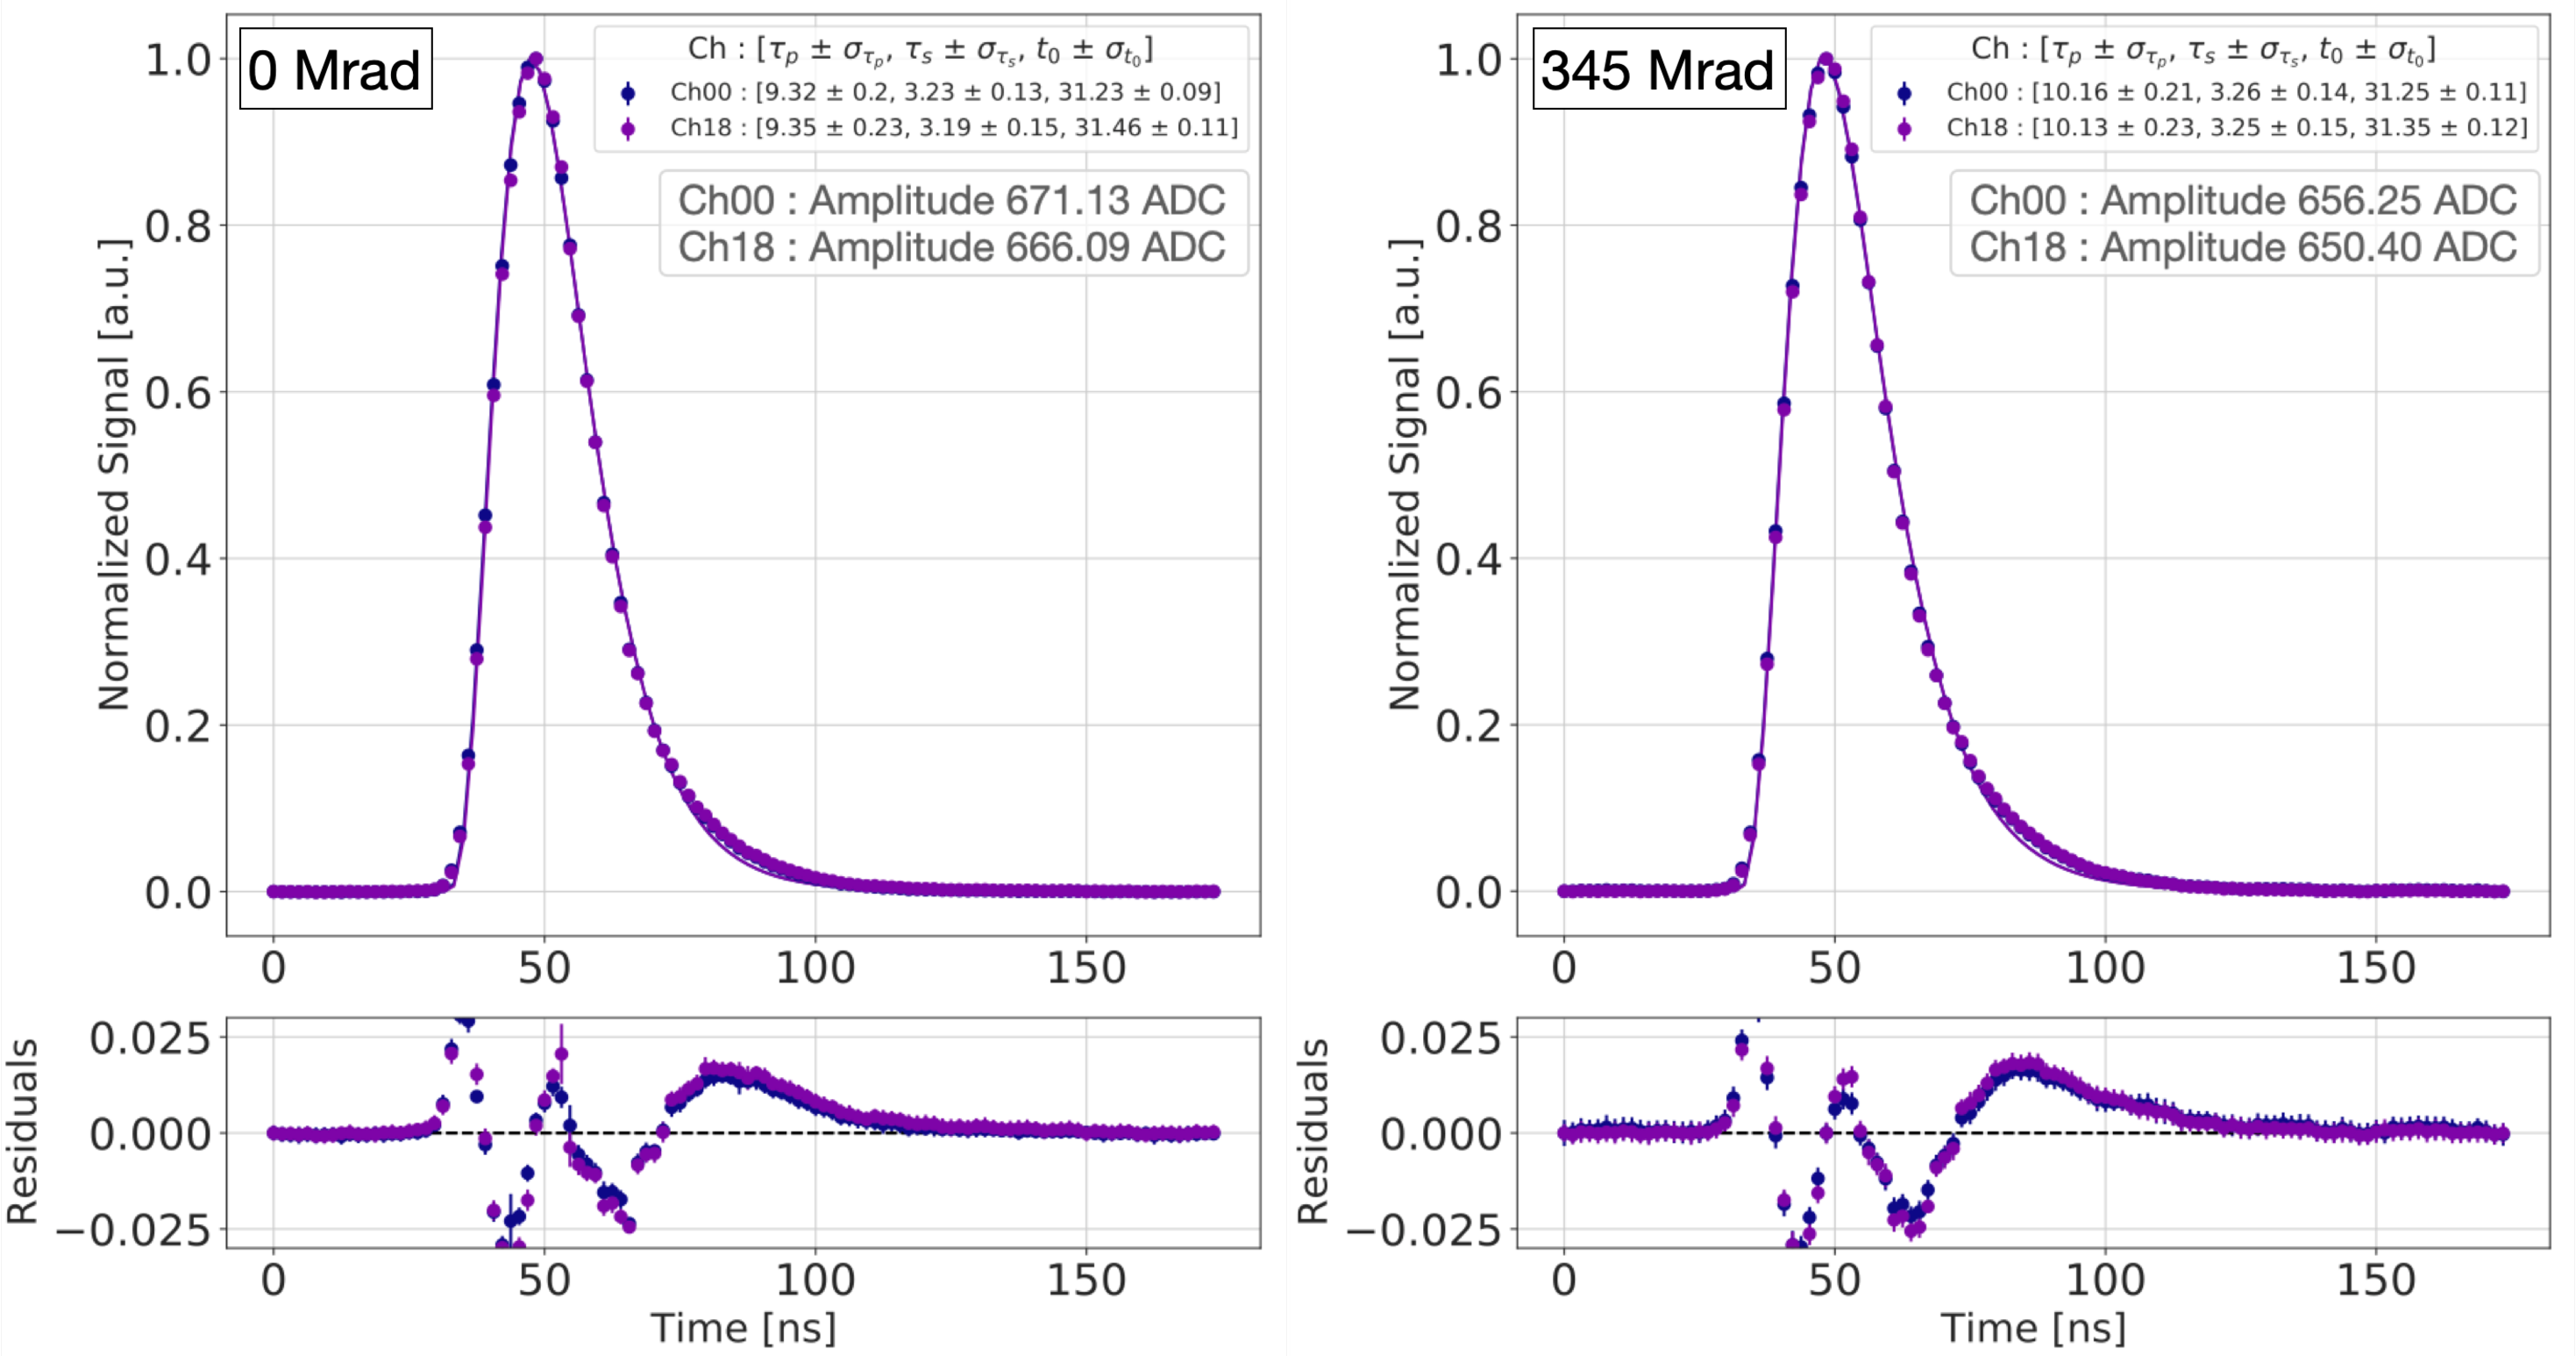
\includegraphics[width=0.7\linewidth]{Figures/HGCAL/TID_SignalShape.pdf}
    \caption{Normalised signal pulse recorded by 2 exemplary channels at the beginning (left) and at the end of the TID irradiation campaign. No degradation is observed in the signal shape, the rising and falling edge characteristic times don't show any significant variation.}
    \label{fig:TID_SignalShape}
\end{figure}

\begin{figure}
    \centering
    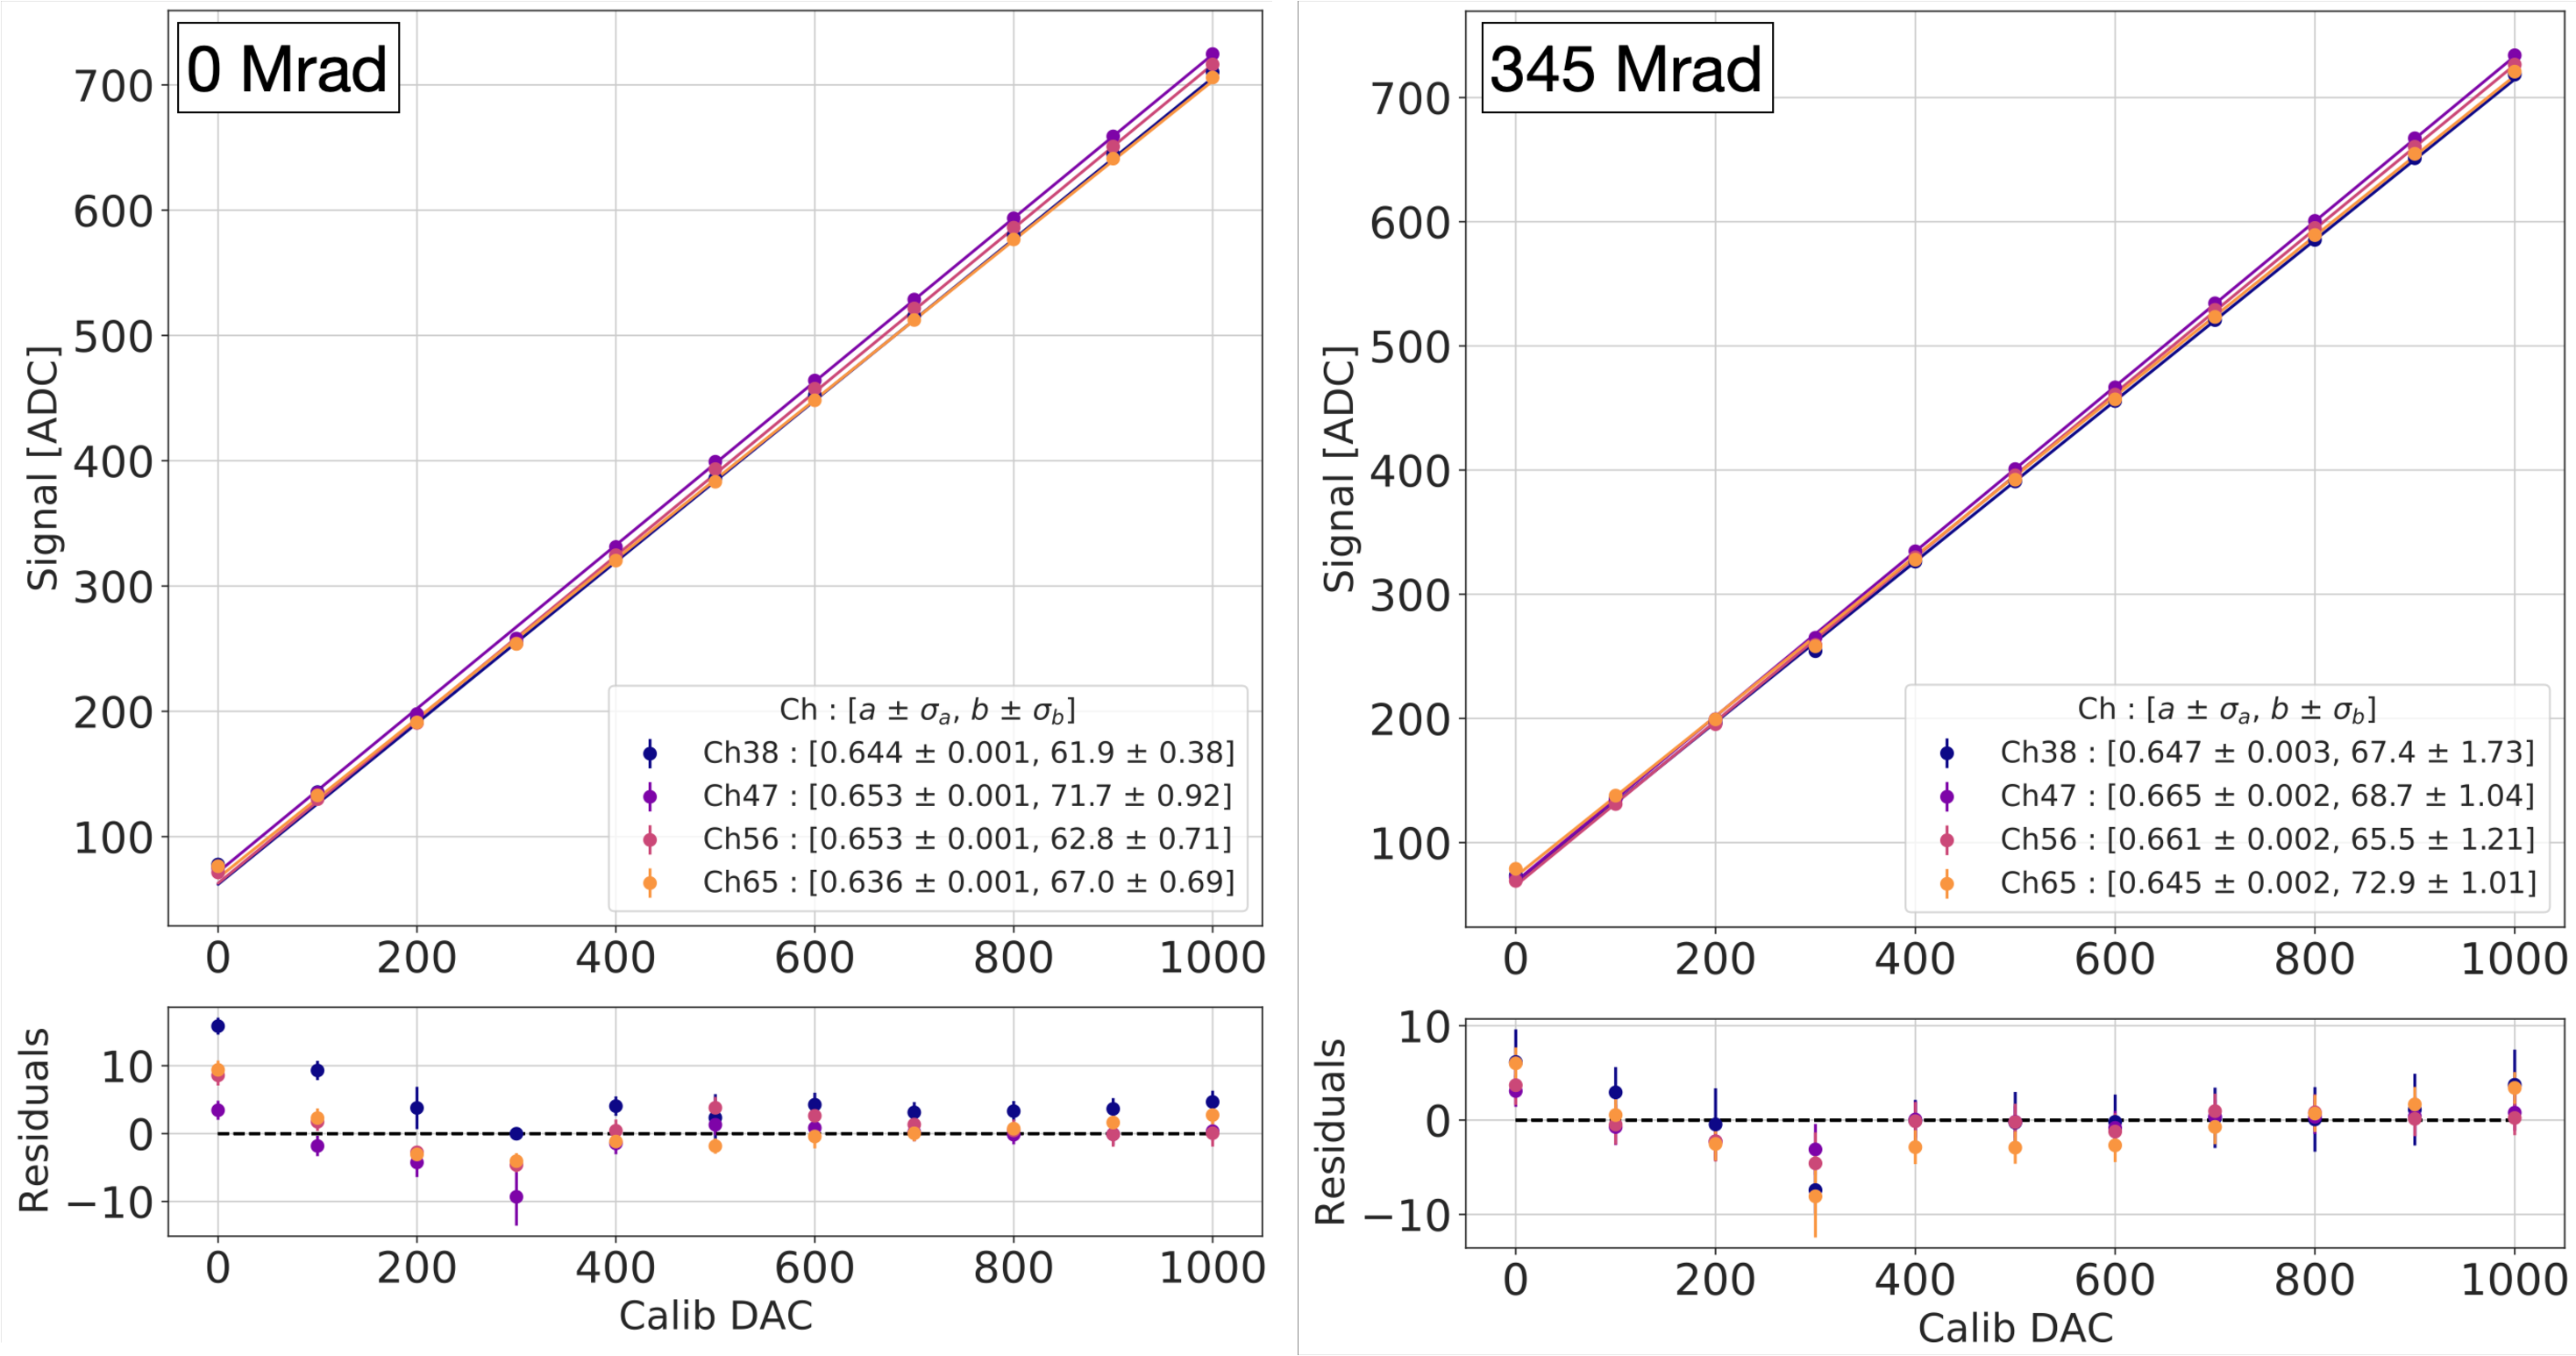
\includegraphics[width=0.7\linewidth]{Figures/HGCAL/TID_ADCLinearity.pdf}
    \caption{Linear dependence of the measured signal amplitude on the injected input charge parameter \texttt{Calib\_DAC} for 4 representative channels of the HGCROC3 at the beginning (left) and at the end (right) of the TID irradiation campaign.}
    \label{fig:TID_ADCLinearity}
\end{figure}

\begin{figure}
    \centering
    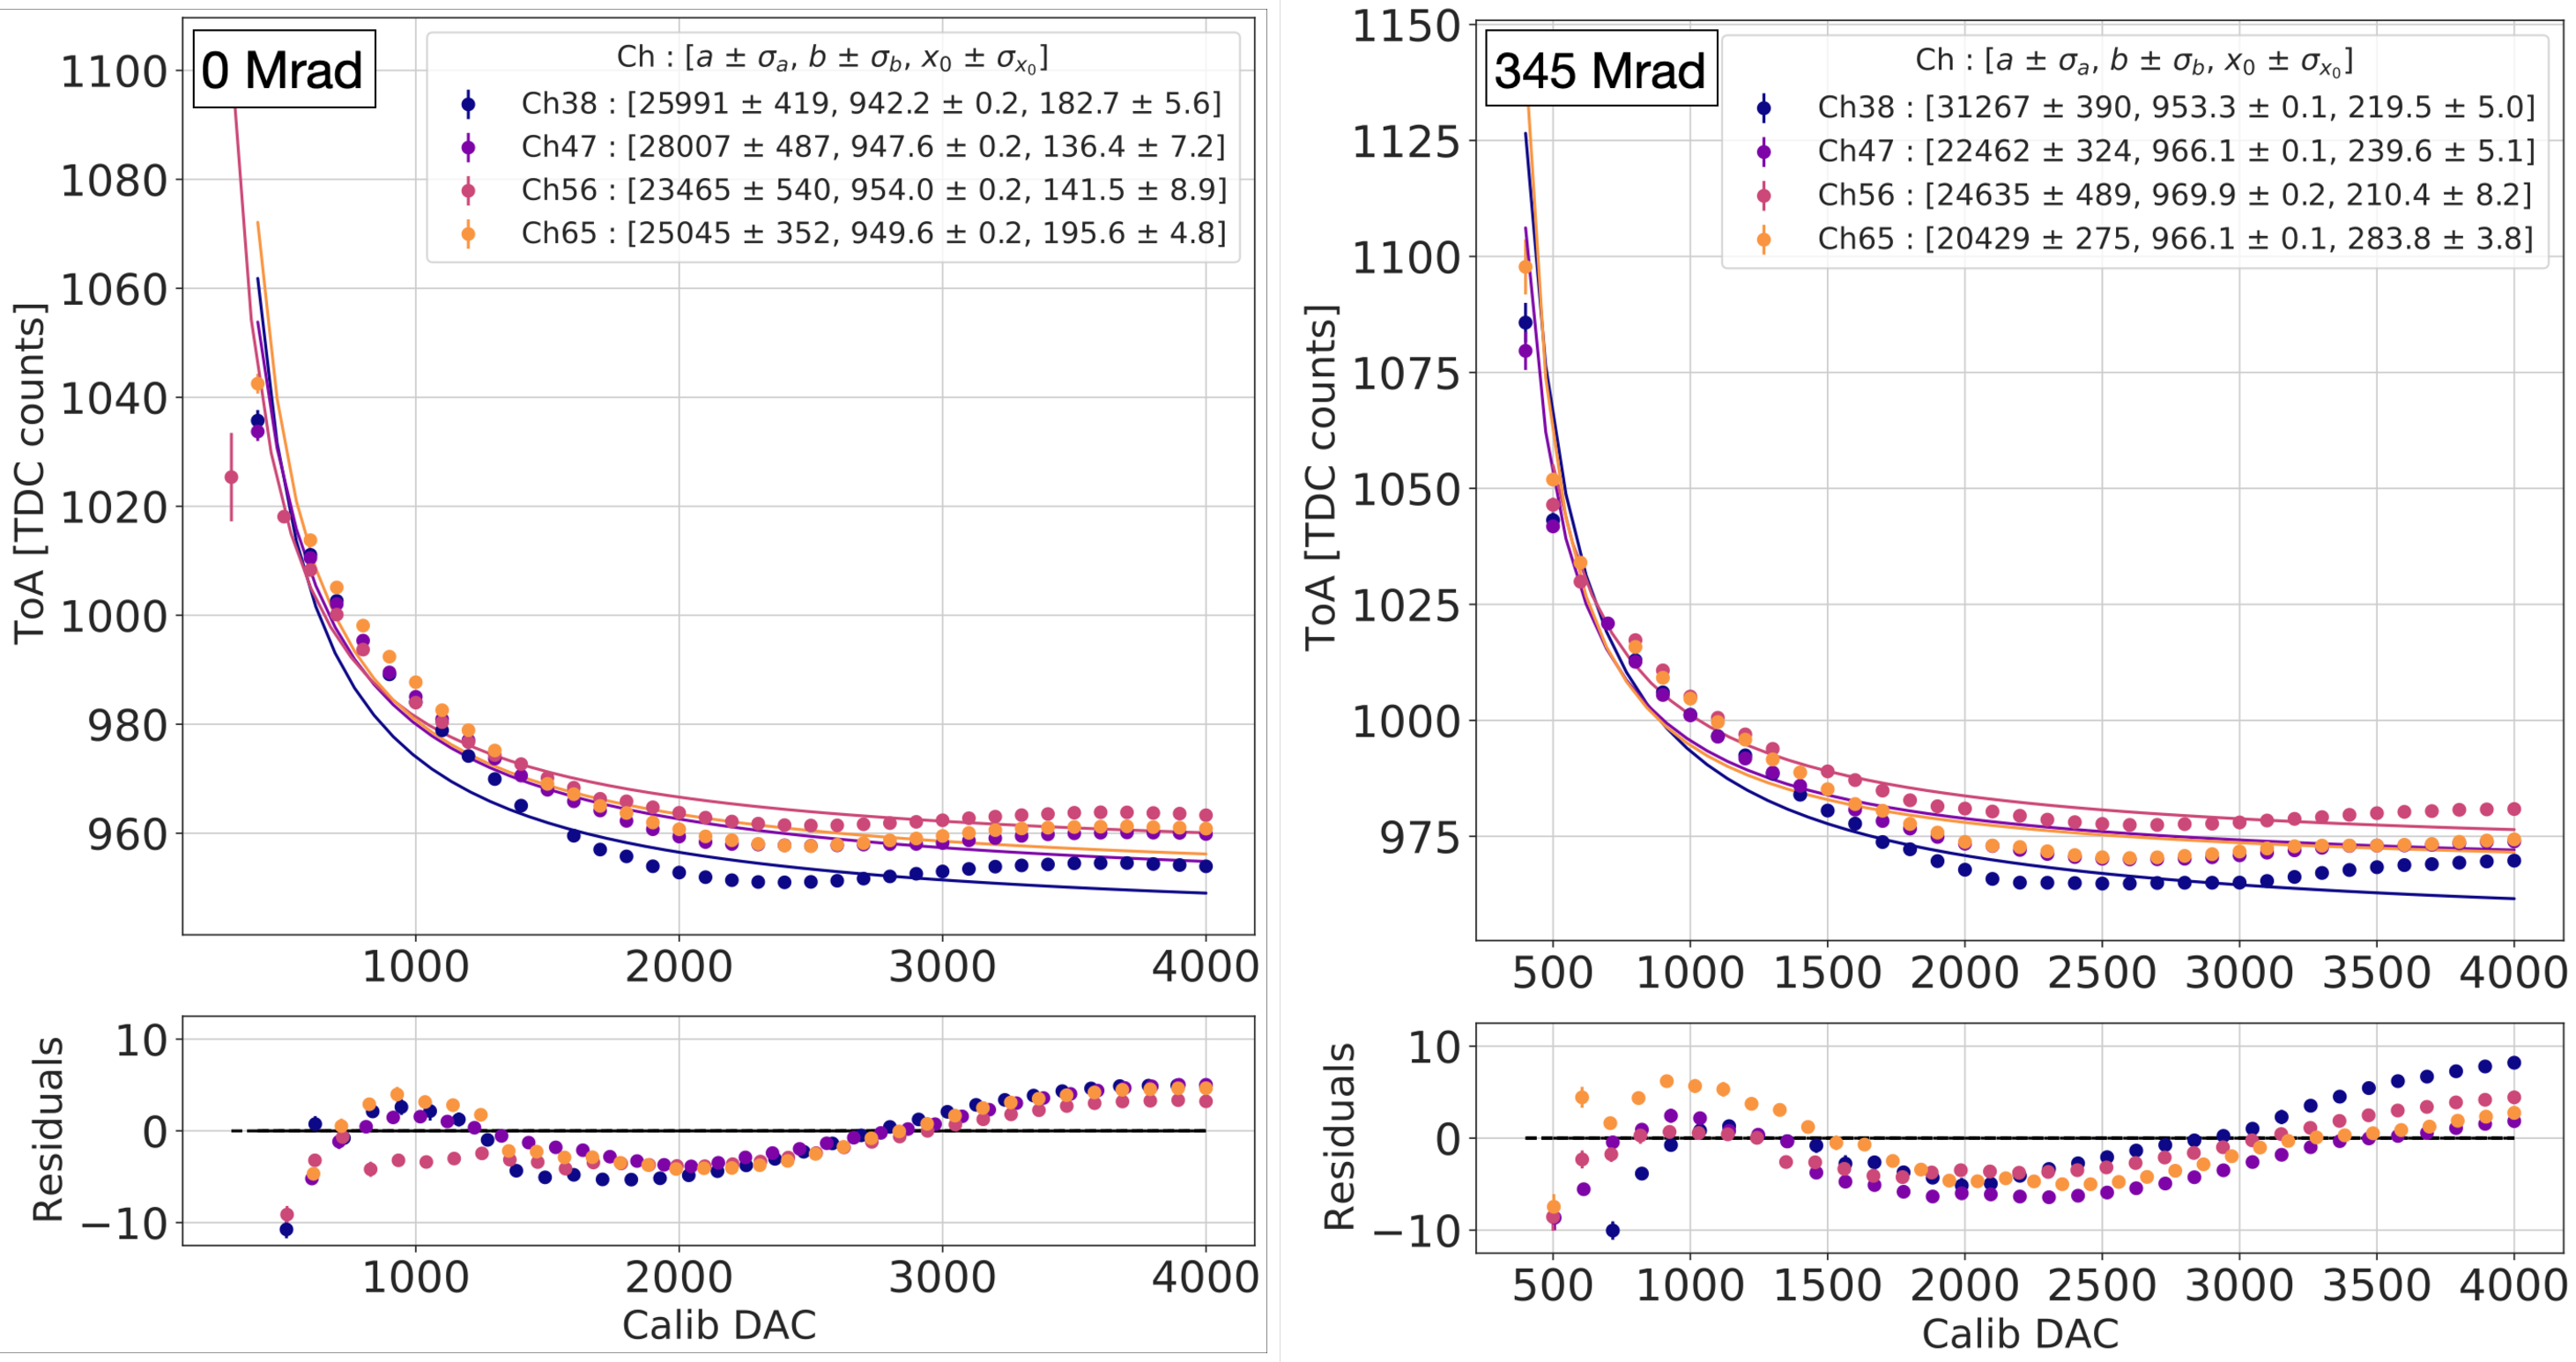
\includegraphics[width=0.7\linewidth]{Figures/HGCAL/TID_TimeWalk.pdf}
    \caption{Time walk curve for the ToA as a function of the injected input charge parameter \texttt{Calib\_DAC} for 4 representative channels of the HGCROC3 at the beginning (left) and the end (right) of the irradiation.}
    \label{fig:TID_TimeWalk}
\end{figure}

\bigbreak

The TID radiation leads to performance degradation in terms of electronics noise: a +$20\%$ increase in the noise is observed at the end of the exposure. Figure~\ref{fig:TID_Noise} shows the distribution of the preamplifier noise for the 72 normal channels of the HGCROC3 at the beginning and at the end of the TID irradiation campaign: from an initial value of 1.4~ADC counts, the noise mean reaches 1.75~ADC counts after $345\,\textrm{Mrad}$ dose. 

The noise increase can significantly impact the HGCROC3 performance, reducing the precision of both the ADC and TDC measurements and affecting the particle reconstruction capabilities. This effect will sum up to the evolution of the silicon sensor noise during radiation exposure and needs to be accounted for in the simulation of the end-of-life detector performance.

% The evolution of the preamplifier noise distribution for the 72 channels of the HGCROC3 is shown in Fig.~\ref{fig:noiseevolution} as a function of the injected dose. A +$20\%$ increase - from 1.5 to 1.8 ADC counts - of the noise mean after $345\,\textrm{Mrad}$ dose is observed, with a -$5\%$ recovery already after 12 hours of annealing. Further studies will be conducted to simulate the effects of the annealing taking place in between consecutive data taking runs.

\begin{figure}
    \centering
    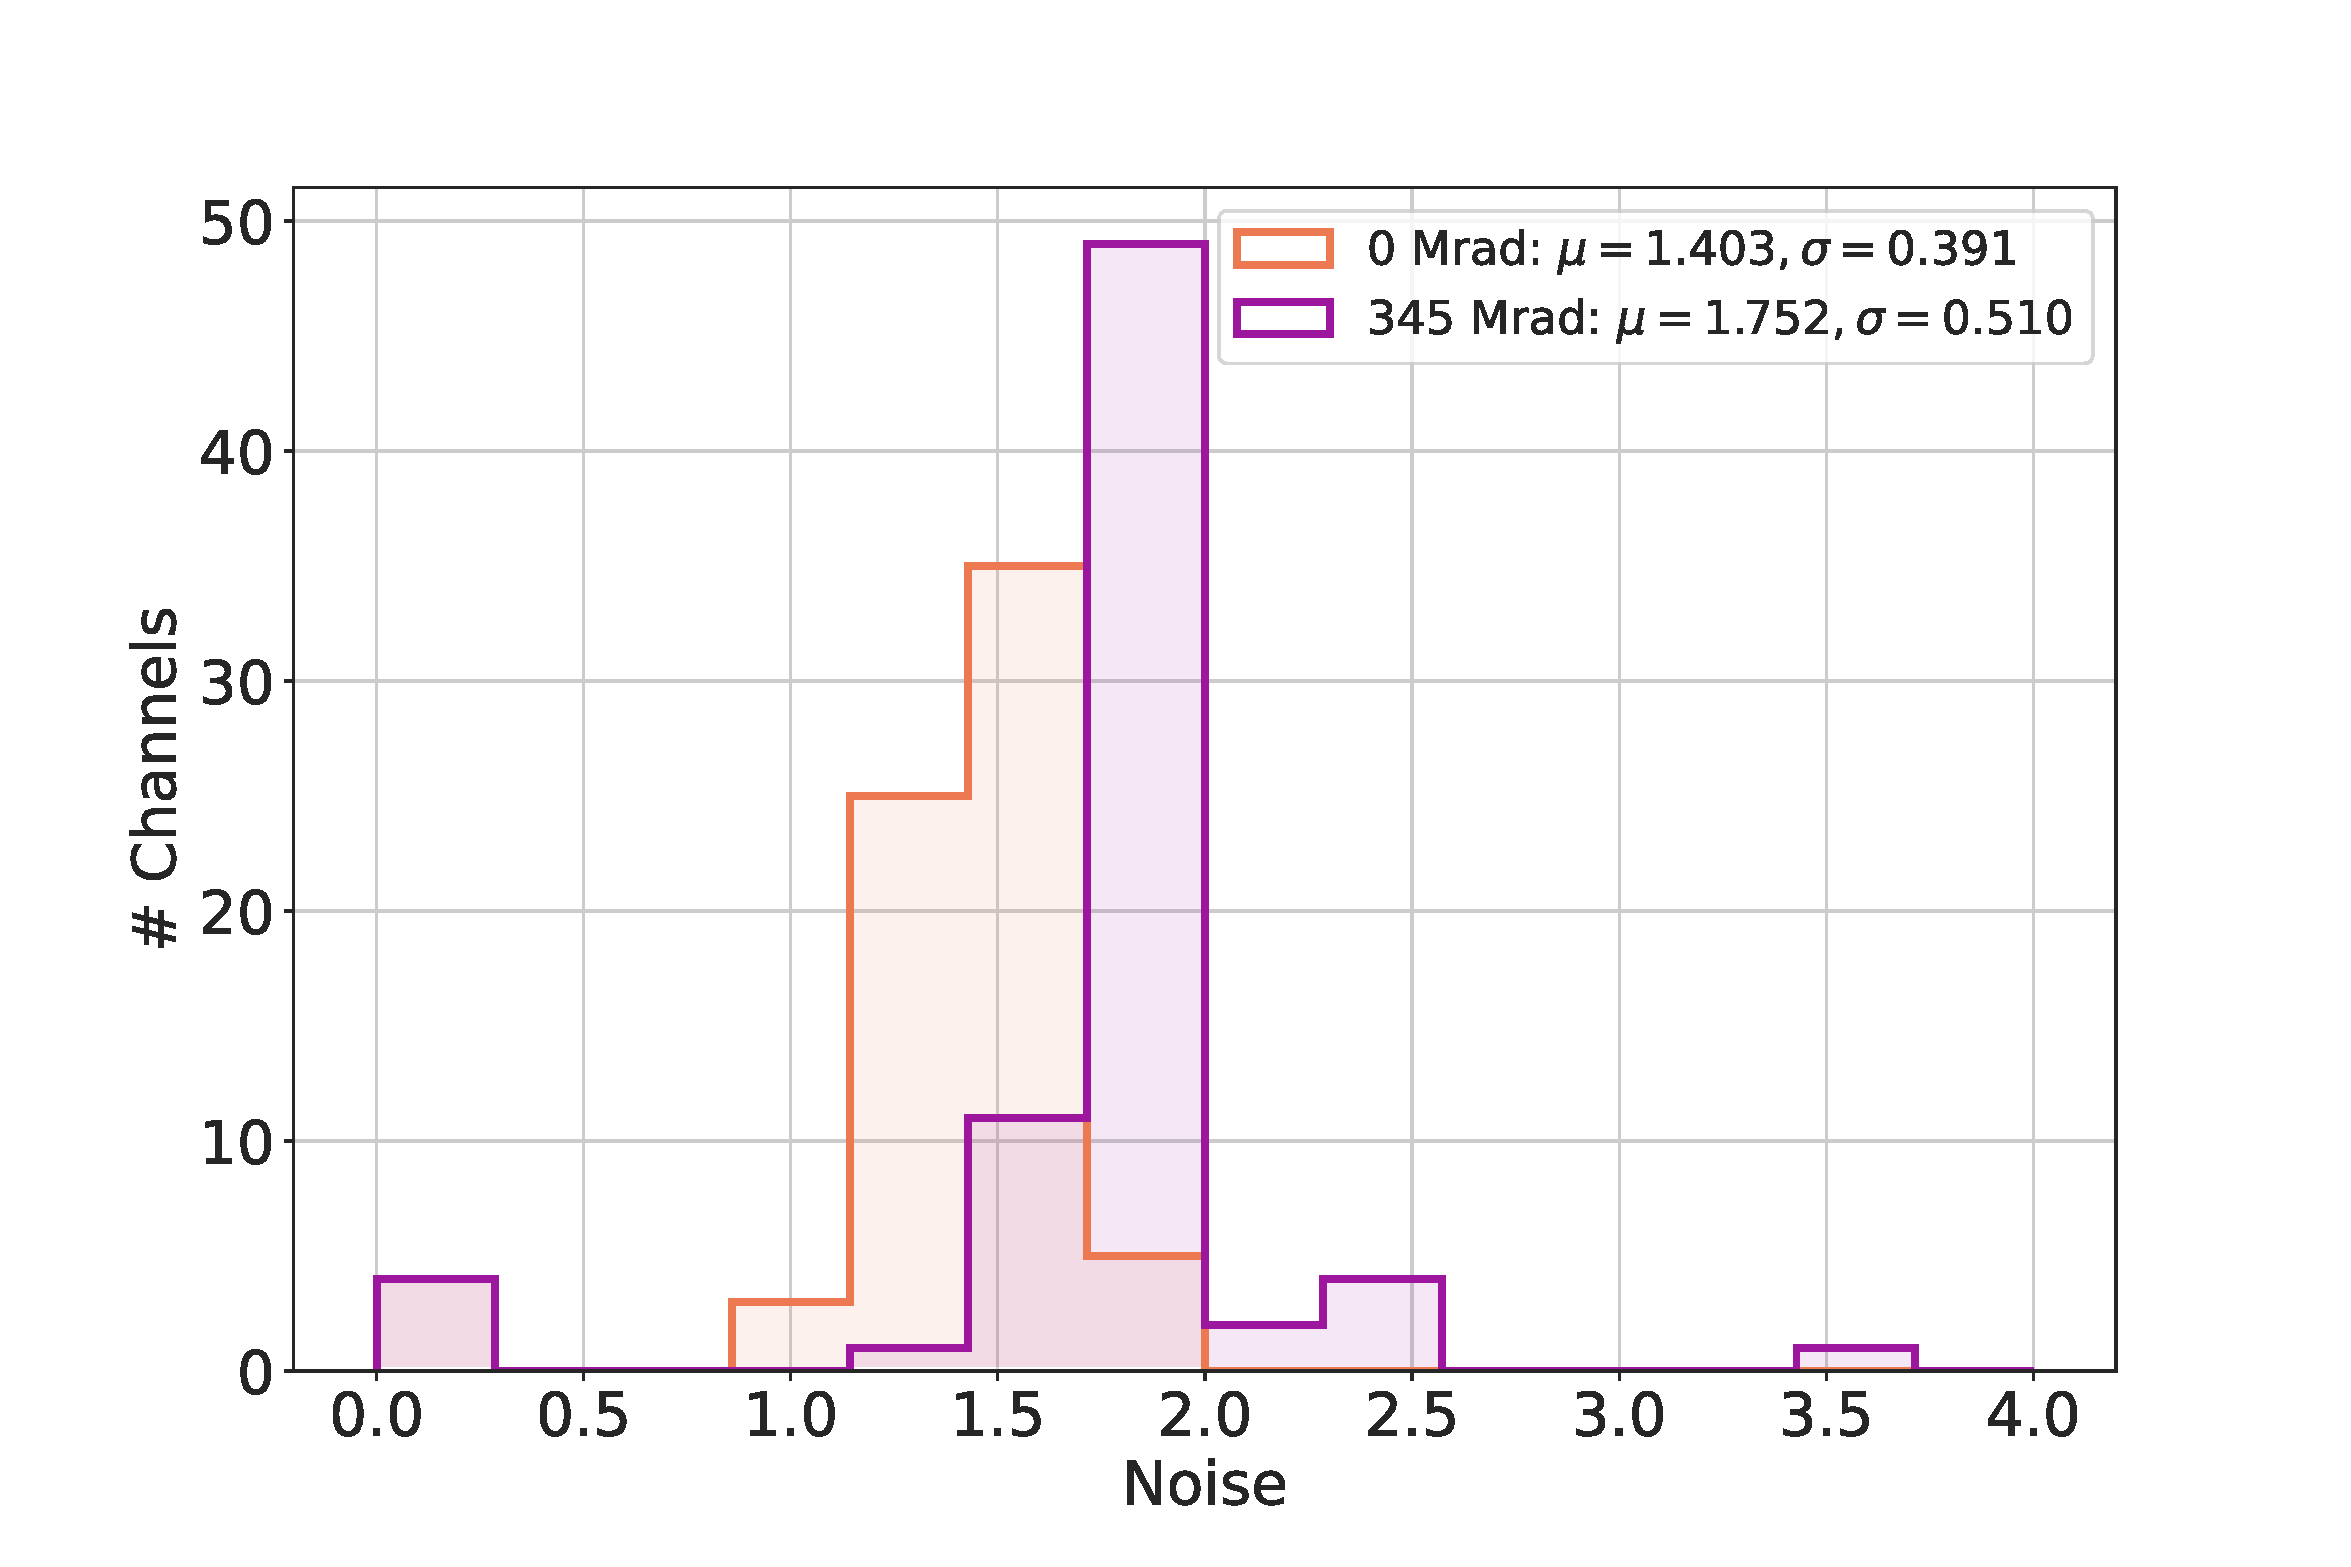
\includegraphics[width=0.65\linewidth]{Figures/HGCAL/TID_Noise.pdf}
    \caption{Distribution of the preamplifier noise for the 72 normal channels of the HGCROC3 at the beginning and at the end of the TID irradiation campaign. An average +$20\%$ increase in the noise is observed. The 4 zero-noise channels in the first bin are already present at the beginning of the irradiation and are due to imperfect chip manufacturing.}
    \label{fig:TID_Noise}
\end{figure}

\subsubsection{Power consumption}
\label{subsubsec:Power consumption}

The power consumption of the HGCROC3 device has been investigated during the exposure time, in terms of bias voltage and current in the analog and the digital components of the chip separately.

The bias voltage shows a stable behaviour, while the current exhibit a +$25\%$ (+$8\%$) peak in the analog (digital) part corresponding to a dose of $10\;\textrm{Mrad}$. This large variation is followed by a slow decrease during the radiation exposure, as illustrated in Figure~\ref{fig:TID_Power}.

\begin{figure}
    \centering
    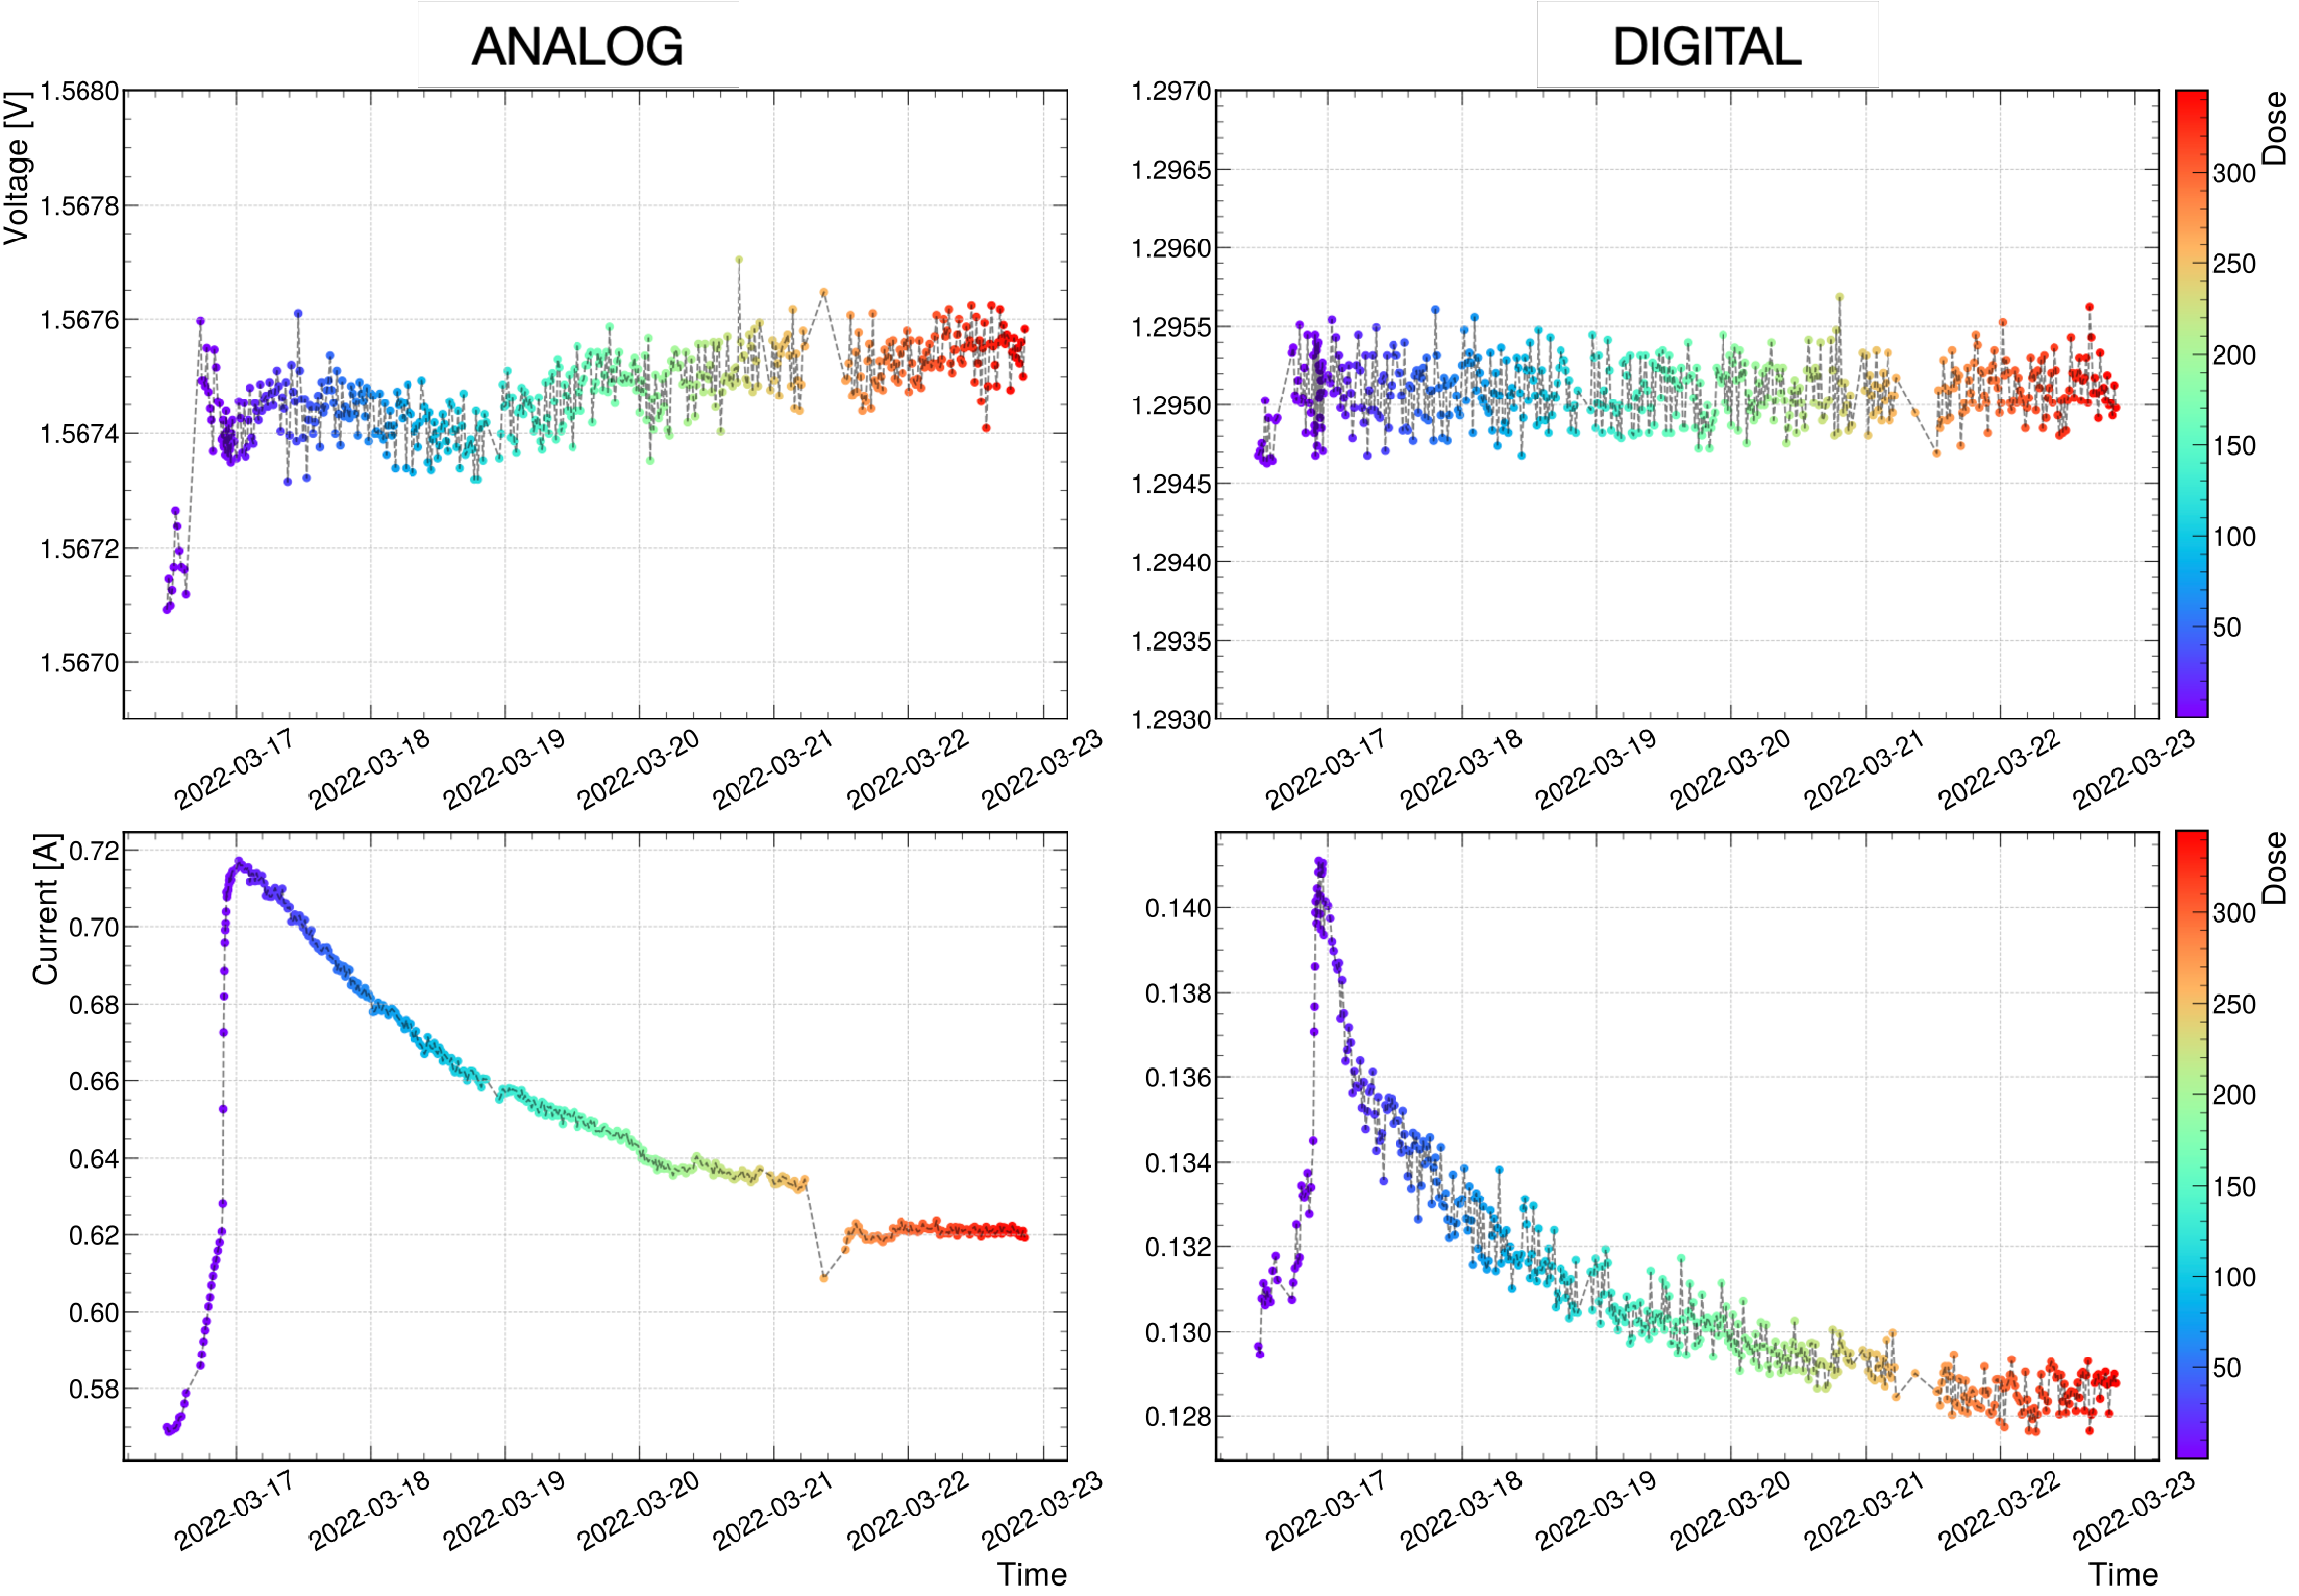
\includegraphics[width=0.99\linewidth]{Figures/HGCAL/TID_Power.pdf}
    \caption{Measurement of the analog and digital power consumption of the HGCROC3 during the radiation exposure as a function of the time and the injected dose.}
    \label{fig:TID_Power}
\end{figure}

\bigbreak

The process causing the current increase is well documented in the literature and it is related to the presence of leakage current in the transistors. 
As illustrated in Figure~\ref{fig:TID_Transistors}, when transistors are exposed to ionizing radiation, such as X-rays, the particles crossing the device can create electron-hole (e-h) pairs in the silicon substrates. Since the electrons have a high mobility, they are quickly removed, while holes are trapped in low-energy traps and the build up of charge creates a distribution of positive charge close to the interface of the gate oxide, resulting in a voltage threshold shift and a leakage current. 

\bigbreak

Small size transistors, such as the ones employed in the digital compartment of the HGCROC3, are usually more affected by the leakage current; however, the effect is expected to decrease with lower dose rate, hence the digital power consumption peak in the HGCROC3 is estimated to be within the acceptable limits and does not constitute a major concern.

On the contrary, the effects of the leakage current on large size transistors, such as the ones employed in the analog part of the HGCROC3, are expected to be significantly reduced. For this reason, the unexpected analog current increase observed during the TID irradiation campaign arouses suspicions about the circuit and deserves a closer investigation.

\bigbreak

Additional TID irradiation campaigns have been performed on various HGCROC3 prototypes in order to understand the source of the analog current increase. 
Table~\ref{tab:TID_Current} reports the results on three devices, irradiated under different conditions of dose rate and temperature.
The results confirm the presence of an current increase in all devices, both in the analog and in the digital part of the chip. The digital increase is stable and not affected by temperature nor dose rate in the investigated range. The analog increase doesn't show dependence on the dose rate, but the peak is reduced at lower temperature.

In order to identify the region of the circuit responsible for the current increase, the power consumption is measured under different settings, by consecutively switching off different parts of the ADC analog chain. The analog current increase is still present when the full ADC chain is not connected, pointing to a possible source of leakage current in the TDC chain.

\bigbreak

Further investigation has been conducted on the irradiated devices in order to locate the source of the leakage current. With the help of a thermal camera it has been possible to highlight the regions of the chip where the current was higher than expected and the leakage source was confirmed to be coming from the TDC component.
The study and simulation of the TDC circuit has finally pointed to a floating input node left in high impedance when no conversion is happening.
% The input voltage should be fixed either to Vgnd=0 or Vdd=1 V, but the leakage current can shift the input value and when A=0.5 V there is current flowing in the circuit. 
This doesn't affect the TDC operations but leads to high leakage current in the downstream NOR gate. Simulations of the circuit can reproduce a current that is compatible with the one observed during the irradiation campaigns.
A correction for this defect has been included the HGCROC3b design.

\begin{figure}
    \centering
    \subfloat[]{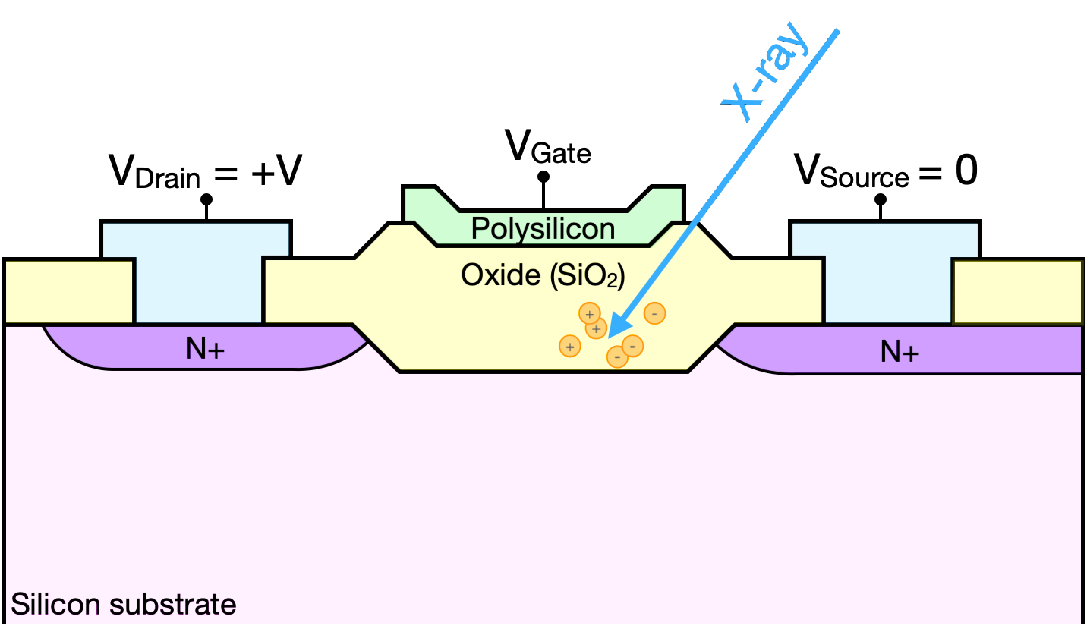
\includegraphics[width=0.32\linewidth]{Figures/HGCAL/TID_Transistors1.pdf}}
    \subfloat[]{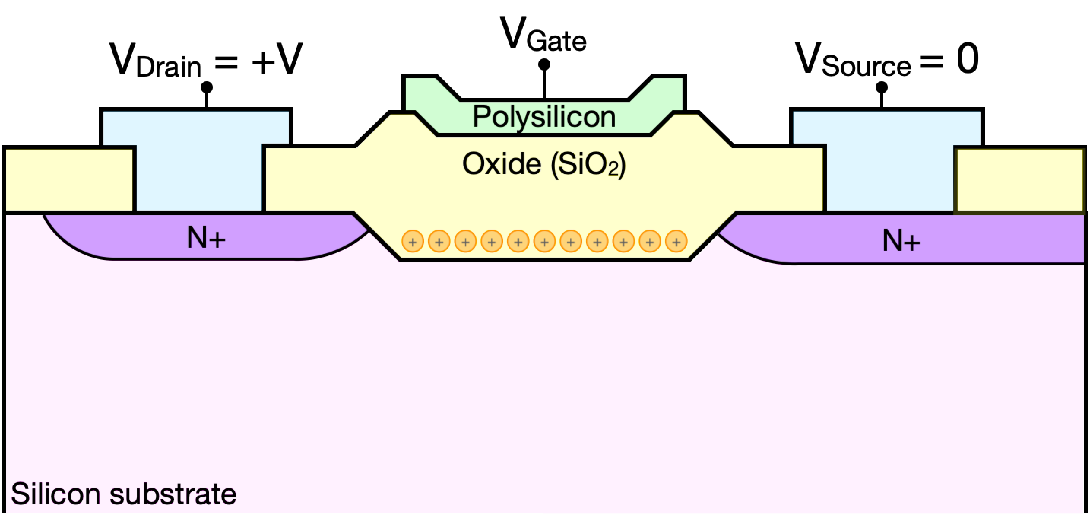
\includegraphics[width=0.32\linewidth]{Figures/HGCAL/TID_Transistors2.pdf}}
    \subfloat[]{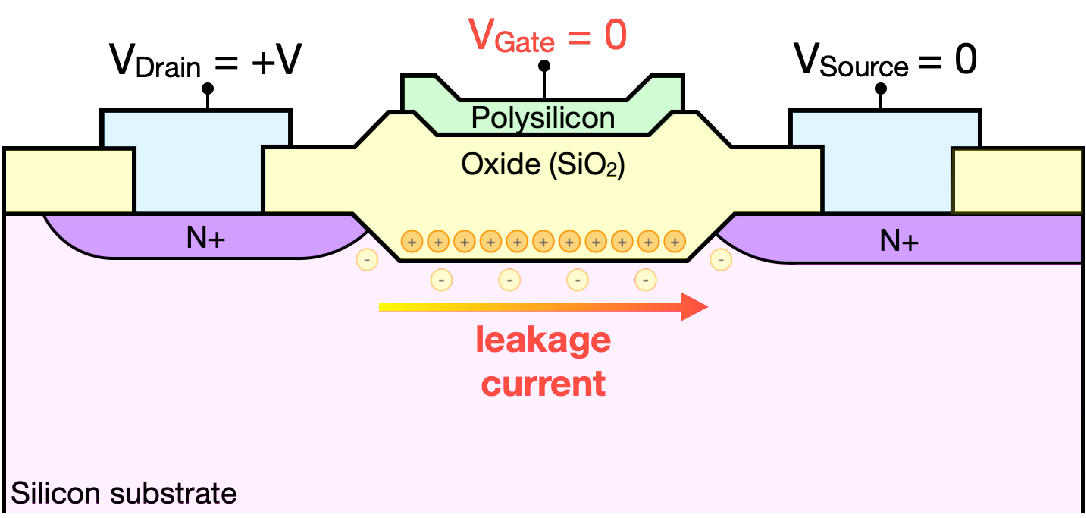
\includegraphics[width=0.32\linewidth]{Figures/HGCAL/TID_Transistors3.pdf}}
    \caption{Illustration of the TID damage in transistors due to hole trapping in the silicon oxide ($\textnormal{SiO}_2$). A ionising particle, like X-rays, crossing the device creates e-h pairs (a): electrons have a high mobility and are quickly removed, while holes are trapped in low-energy traps (b). The build up of charge creates a distribution of positive charge close to the interface of the gate oxide, leading to voltage threshold shifts or leakage current (c).}
    \label{fig:TID_Transistors}
\end{figure}

\begin{table}
    \centering
    \begin{tabular}{c|c|c|c|c}
        \hline
        \hline
        Chip Number & Dose Rate & Temperature & Analog Increase & Digital Increase \\
        \hline
        ROC 003 & 2.5 Mrad/h & $+20^{\circ}$C & 0.40 A & 0.015 A \\
        ROC 000 & 2.5 Mrad/h & $-10^{\circ}$C & 0.175 A & 0.015 A \\
        ROC 015 & 0.3 Mrad/h & $-10^{\circ}$C & 0.175 A & 0.015 A \\
        \hline
        \hline
    \end{tabular}
    \caption{Results from three TID campaigns performed on prototypes of HGCROC3 with different dose rate and temperature conditions for the investigation of the analog and digital current increase during the radiation exposure.}
    \label{tab:TID_Current}
\end{table}

\bigbreak

The TID irradiation campaign has proven to be fundamental in evaluating the radiation tolerance of the HGCROC3 up to $200\,\textrm{Mrad}$. The successful execution of this campaign under various conditions has provided crucial insights into the device resilience in radiation-prone environments. 
Moreover, it has highlighted the presence of a floating input node in the TDC circuit, an issue that could be rectified before finalising the HGCROC3b design and initiating large-scale production. 

%%%%%%%%%%%%%%%%%%%%%%%%%%%%%%%%%%%%%%%%%%%%%%%%%%%%%%%%%%%%%%%%%%%%%%%%%%%%%%%%%%%%%%%%%%%%
%%%%%%%%%%%%%%%%%%%%%%%%%%%%%%%%%%%%%%%%%%%%%%%%%%%%%%%%%%%%%%%%%%%%%%%%%%%%%%%%%%%%%%%%%%%%
%%%%%%%%%%%%%%%%%%%%%%%%%%%%%%%%%%%%%%%%%%%%%%%%%%%%%%%%%%%%%%%%%%%%%%%%%%%%%%%%%%%%%%%%%%%%
%%%%%%%%%%%%%%%%%%%%%%%%%%%%%%%%%%%%%%%%%%%%%%%%%%%%%%%%%%%%%%%%%%%%%%%%%%%%%%%%%%%%%%%%%%%%

\subsection{Single Event Effect}
\label{subsec:Single Event Effect}

The Single Event Effect (SEE) irradiation test aims at evaluating the radiation damage induced by a single energetic particle on electronic devices. Differently from the TID irradiation test, the SEE induces very localised and non cumulative effects causing potential malfunctioning inside the data-processing system with multiple consequences. Given the stochastic nature of the effect, it can happen at any moment since the beginning of the operation.

In the LHC radiation environment, SEE events could become an important issue, not much because a small fraction of the enormous data stream would be corrupted, but because some vital detector control functions could be lost due to memory upsets. It is thus important to preserve the device from this kind of potential danger, by implementing tools to secure the static memory registers storing the logic configuration.

\bigbreak

A SEE is caused by a very high energy deposition in a small volume of the electronic device. The single ionizing particle crossing the silicon device releases charge and creates electron-hole pairs that are collected at one of the microcircuit nodes and produce a temporary current transient in the circuit. 

% Three possible consequences can occur:
% \begin{itemize}
%     \item [-] \textit{Single Event Upset} (SEU): a bit storing the logic information is flipped,
%     \item [-] \textit{Single Event Transient} (SET): a shift in the string of bits,
%     \item [-] \textit{Single Event Latch-up} (SEL): a short circuit in part of the device causing permanent damage.
% \end{itemize}

% \begin{itemize}
%     \item [-] Single Event Upset (SEU): digital error, or bit flip.
%     \item [-] Single Event Transient (SET): analog error,  or bit shift.
%     \item [-] Single Event Latch up (SEL): permanent damage of the device.
% \end{itemize}

Three possible consequences can occur:
\begin{itemize}
    \item The \textit{Single Event Upset} (SEU) is a non-destructive phenomenon inducing a flip in the bits that store the logic information. The cause lies in the digital part of the electronic device, based on the transistor technology, where the one-bit memory element is designed to have two possible stable states: 0 or 1. An SEU event appears as an error in the information stored either inside the dynamic or the static memory register, i.e. a bit flip from 0 to 1 or the opposite.
    \item The \textit{Single Event Transient} (SET) happens when the charge collection creates a spurious current signal changing one of the clock frequencies of the device. The frequency is usually provided to the chip by an analog synthesizer inside the PLL module: if a glitch affects the output signal of this module, all the activities in the chip can suffer from a temporary loss of synchronization, resulting in undesirable circuit response that can vary depending on the circuit topology and the amount of charge collected.
    \item The \textit{Single Event Latch-up} (SEL) is a permanent destructive event where the current induced by the incident particle is so high to create a short circuit in part of the circuit.
\end{itemize}

The magnitude of these effects and their occurrence depends on the circuit topology and on the characteristics of each particle interaction, from the charge collection efficiency to the time constants of the perturbation effect. 

\bigbreak

\begin{figure} [b]
    \centering
    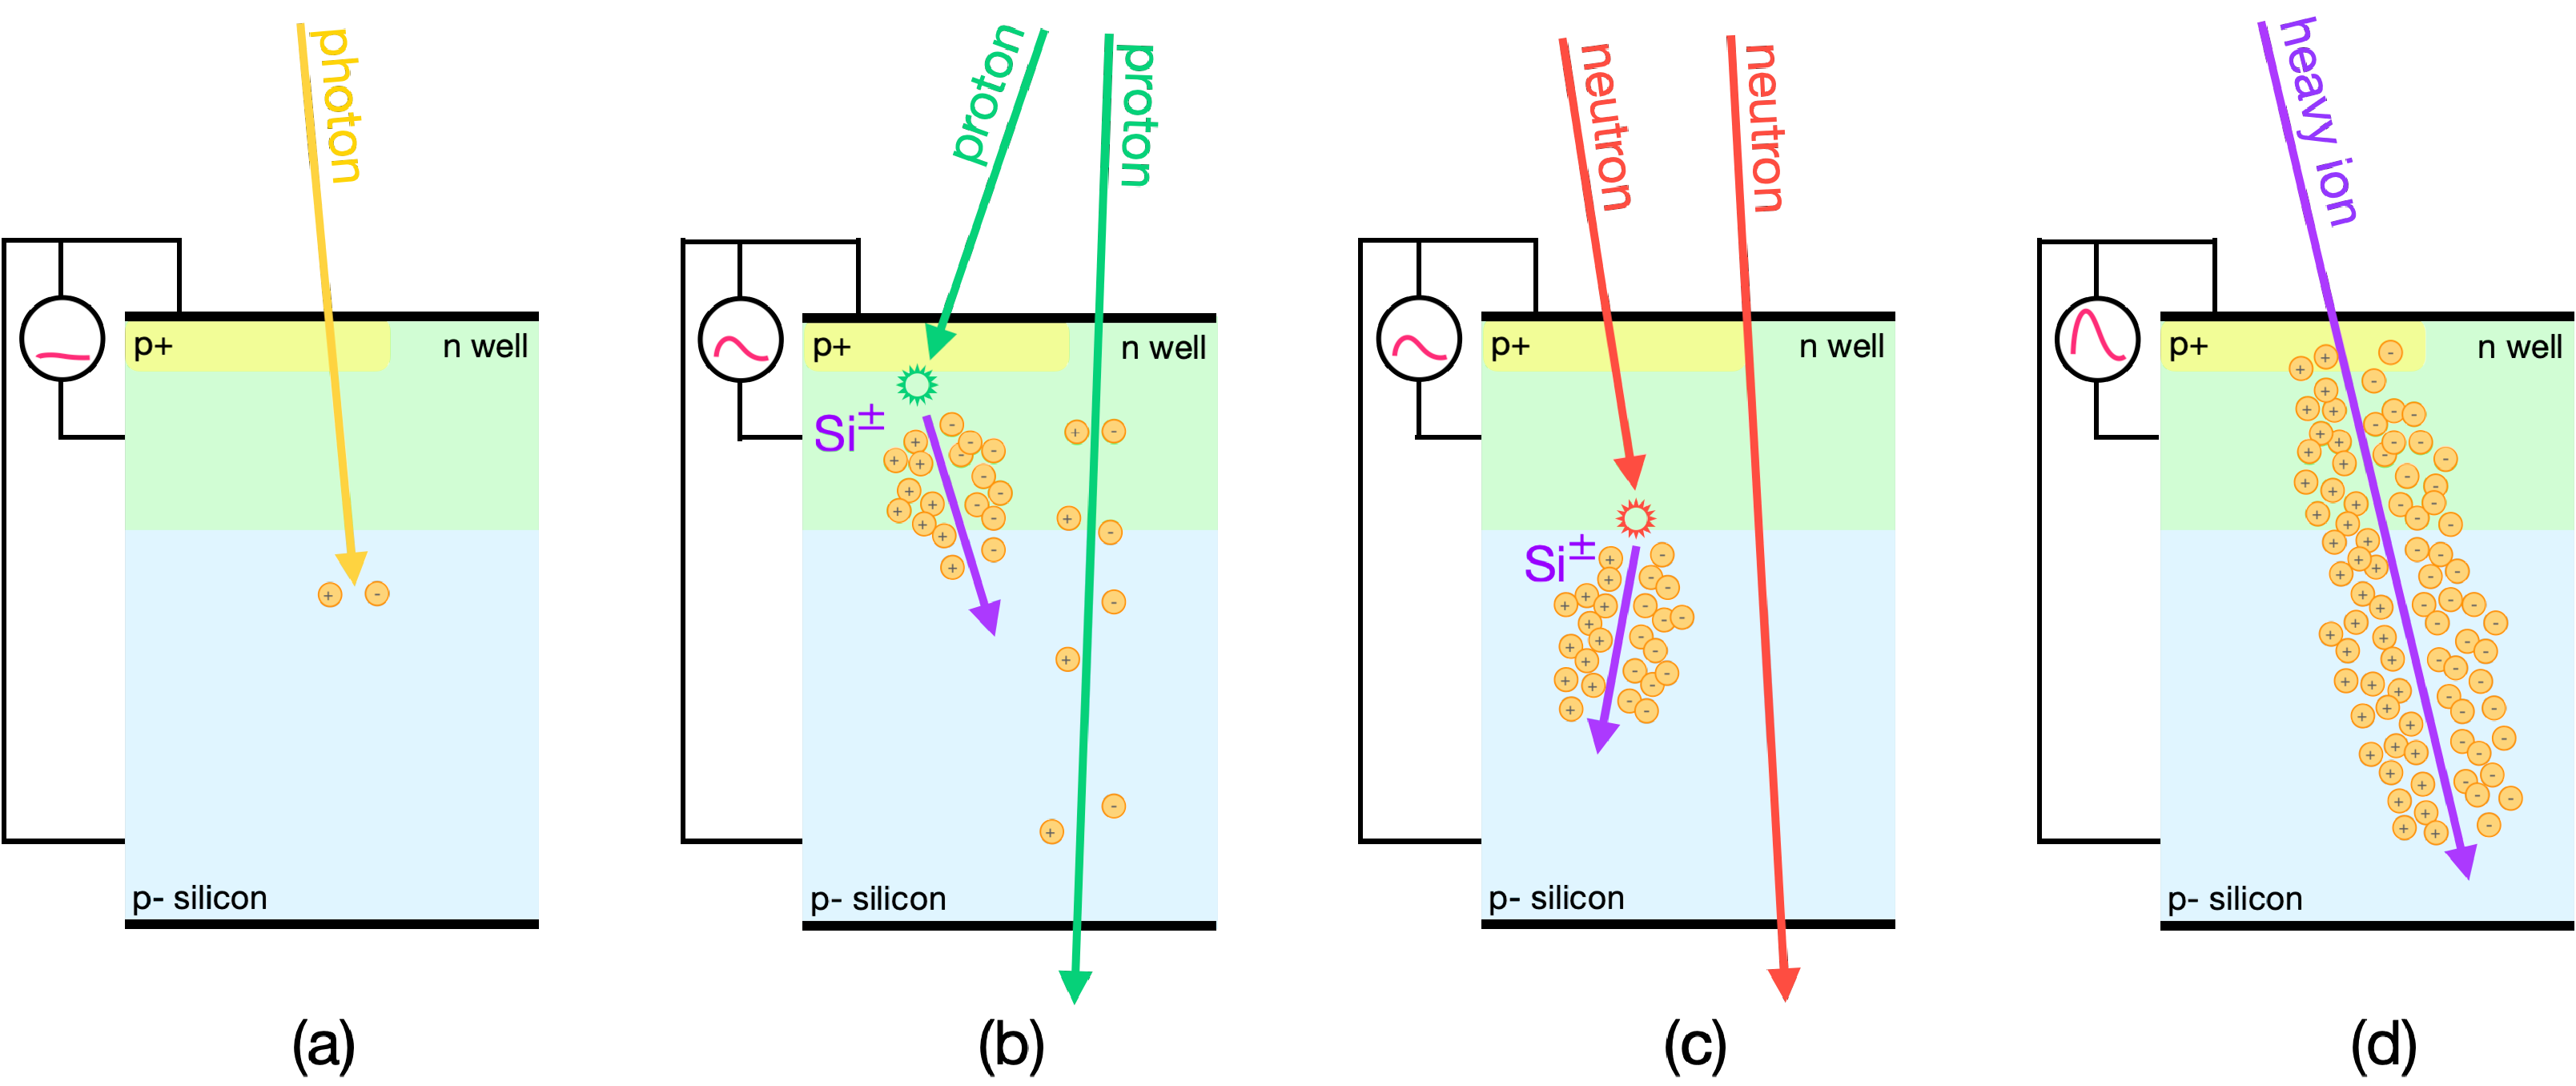
\includegraphics[width=0.99\textwidth]{Figures/HGCAL/SEE_ParticleInteraction.pdf}
    \caption{Caption}
    \label{fig:SEE_ParticleInteraction}
\end{figure}

In the LHC radiation environment different particles can hit the HGCAL read-out system, with different effects depending on the ionization process and the density of e-h pairs produced in the interaction. 
However, the main radiation damage on HGCROC3 is expected to mainly come from by Minimum Ionizing Particles (MIP), like protons or light hadrons. 

In order to test the HGCROC3 radiation hardness against SEE, two irradiation campaigns have been performed with heavy ions and protons. 

% The major energy loss mechanisms for charged particles inside matter are ionization and bremsstrahlung, where the former is much more predominant. 
% The energy loss $dE/dx$ is described through the Stopping Power or Linear Energy Transfer (LET), which is defined as the amount of incident particle energy deposited per unit track length in the material of interest.
% The energy loss of a minimum ionizing particle (e.g. a proton of about 2~GeV) in silicon is about 3.9~MeV/cm. This energy loss increases rapidly with decreasing energy of the particle, following the Bethe-Bloch formula, up to reach a maximum around 100~keV of kinetic energy.
% The ionization directly induced by protons is usually not dense enough to provoke an upset in the circuit, but the highest damage is in fact due to indirect ionization: when a proton hits the silicon substrate, it can produce a nuclear interaction and give part of its energy to a nucleus of Silicon. 
% This charged nuclear recoil is actually a ionizing particle with low energy (usually $<$ 10~MeV) and a limited range ($<$ 10~$\mu$m), but it has enough energy to ionise the substrate and create current inside the circuit.
% The probability of nuclear interaction caused by protons is low, around $~10^{-5}$, but given the high flux of particles, the probability of having an SEE is not negligible.
% https://indico.cern.ch/event/635099/contributions/2570672/attachments/1456364/2249943/Single_Event_Effecs_Radiation_Course_May_2017_SEE_CBP.pdf

\subsubsection{SEE with Heavy Ions}
\label{subsubsec:SEE with Heavy Ions}

The first SEE campaign has been performed using a beam of low-energy heavy ions at the UCL cyclotron (Louvain).
The facility provides several types of heavy ions with different values of mass-to-charge ratio (M/Q) and Linear Energy Transfer (LET), as shown in Table \ref{tab:SEE_Ions}, at a fixed flux of $10^4\,\textrm{s}^{-1}\,\textrm{cm}^{-2}$.

\begin{table}[]
    \centering
    \begin{tabular}{c | c | c | c}
        \hline
        \hline
        \multirow{2}{*}{Ion} & \multirow{2}{*}{M/Q} & Range & LET \\
        &  & [$\mu$m] & [$\textrm{MeV}/\textrm{mg}/\textrm{cm}^2$] \\
        \hline
        Ne & 3.14 & 202.0 & 3.3 \\
        Al & 3.37 & 131.2 & 5.7 \\
        Ar & 3.33 & 120.5 & 9.9 \\
        Cr & 3.31 & 107.6 & 16.0 \\
        Ni & 3.22 & 100.5 & 20.4 \\
        Kr & 3.35 & 94.2 & 32.4 \\
        Xe & 3.54 & 73.1 & 62.5 \\
        \hline
        \hline
    \end{tabular}
    \caption{List of the available heavy ions at the UCL cyclotron. Each ion is characterised by a different mass-to-charge ratio (M/Q), penetration range in Silicon material, and Linear Energy Transfer (LET).}
    \label{tab:SEE_Ions}
\end{table}
% [FIXME] Add Corrected LET after 70 um of Silicon

\bigbreak

Since the HL-LHC radiation environment will be dominated by light hadrons, like protons and neutrons, some fundamental differences in the particle interactions have to be considered when characterizing a device with heavy ions.
When a light hadron hits the device, it can produce a hadronic interaction and generate a shower of secondary particles and a nuclear recoil - in some cases even several fragments.
This charged nuclear recoil is an ionizing particle with low energy (typically less than $10\,\textrm{MeV}$) and a limited range (below $10\,\mu\textrm{m}$) that travels through the substrate creating electron-hole pairs. The collection of this charge by a node of the circuit can temporarily alter the status of the device.
A heavy ion can simulate the ionization caused by the nuclear recoil, but with a larger range and a bigger energy deposit (Fig.~\ref{fig:sensitivevolume}).

The SEE occurrence depends on the \textit{Sensitive Volume} (SV) of the device, which is the region where the charge collection can contribute to a possible alteration of the circuit:
\begin{itemize}
    \item [-] for a SEU on the digital part, a very fast current signal is required: the digital SV is usually small and there is no radical difference between heavy ions and protons;
    \item [-] for a SET on the analog part, all the signals can have a contribution: the analog SV significantly depends on the particle type, making the heavy-ion irradiation a unreliable estimate in terms of SETs.
\end{itemize}

\begin{figure}[b]
    \centering
    \includegraphics[width=0.85\linewidth]{figures/sensitivevolume.pdf}
    \caption{Difference between light hadrons (protons and neutrons) and heavy ions irradiation: the digital SV (dashed blue line) is typically smaller than the analog SV (dashed pink line).}
    \label{fig:sensitivevolume}
\end{figure}

The heavy ions irradiation is also a very important stress test for SELs: as proposed in \cite{federico}, the absence of latch-ups for high LETs ($\sim$$40\,\textrm{MeV}/\textrm{mg}/\textrm{cm}^2$) will guarantee the robustness of the device against latch ups in an accelerator environment.

During the SEE campaign, the digital components of the HGCROC3 are tested with two measurements: the I2C and the DAQ test.

\vspace{-2.8mm}
\subsection*{I2C test}
 The I2C of the HGCROC3 holds 2573 configuration parameters (8956 bits) that are tested against possible SEUs. All the parameters are protected by the triplication logic - the value of each bit is stored into three different cells - and by the \textit{AutoReload} mode: whenever an SEU happens changing the value of one cell, the I2C sends a command to refresh all the cell values according to the majority vote.
 
 During irradiation all the bits are monitored and the resulting numbers of errors are summarized in Table \ref{tab:I2C}: while multiple bit flips are observed when the \textit{AutoReload} mode is disabled, no bit flip is observed when the \textit{AutoReload} mode is enabled.

\begin{table}[]
    \centering
    \caption{Results of the I2C test when the \textit{AutoReload} is disabe (OFF) or enable (ON).}
    \begin{tabular}{c | c c | c c}
        \hline
        \hline
        % [$\textrm{MeV}/\textrm{mg}/\textrm{cm}^2$]  [$\textrm{part}/\textrm{s}/\textrm{cm}^2$]
        & \multicolumn{2}{c |}{AutoReload OFF} & \multicolumn{2}{c}{AutoReload ON} \\
        Ion & Time [s] & Bit flips & Time [s] & Bit flips \\
        \hline
        Ne & 490 & 55 & 1515 & 0 \\
        Al & 490 & 213 & 1291 & 0 \\
        Ar & 699 & 316 & 1184 & 0 \\
        Cr & 687 & 559 & 879 & 0 \\
        Ni & 678 & 662 & 1289 & 0 \\
        Kr & 507 & 502 & 661 & 0 \\
        Xe & 641 & 130 & 127 & 0 \\
        \hline
        \hline
    \end{tabular}
    \label{tab:I2C}
\end{table}

\vspace{-2.8mm}
\subsection*{DAQ test}
The DAQ test checks for possible SEUs on the Data and Trigger paths (Fig.~\ref{fig:paths}) of the HGCROC3 during the data acquisition. 
The Trigger path is composed by a fixed header and four compressed energy sums.
The Data path is the concatenation of a header, data coming from common mode, normal and calibration channels, the Cyclic Redundancy Check (CRC) - that sums all the previous bits to check the integrity in the transmission -, and a final idle word.
Inside the header, the bunch crossing, event and orbit counters are triplicated, while the remaining data are processed with the \textit{Hamming} encoding, following the logic of \textit{Single Error Correction - Double Error Detection} (SEC-DED).

In a standard acquisition the potential bit flips could get lost among the random noise fluctuations of the data, for this reason a fixed data pattern is transmitted to all the channels and then compared to the output pattern.

During the DAQ test no error is detected in the triplicated counters; just few SEU events are observed on the non-triplicated parts, without raising particular concern since they are just affecting the data and not the state of the chip. 
Due to the poor statistics, it is not possible to extrapolate a reliable estimate for the HL-LHC radiation environment.

Besides few SEUs, several SETs are observed on the analog part of the HGCROC3, changing the output frequency of the PLL and causing link misalignments. Two cases are reported:
\begin{itemize}
    \item [-] short SET: the data transmission fails for just one bit and the rest of the data flow is correct;
    \item [-] long SET: the transmission is lost for longer time, leading to a constant shift in the string of bits; a link realignment is necessary to restore the data flow.
\end{itemize}

In Table \ref{tab:DAQ} a summary of all the SEU and SET events observed during the DAQ test is shown, where it is important to recall that the estimated number of SET events is not reliable under heavy ions irradiation.

No SEL events are observed during the SEE campaign with heavy ions.

After the SEE campaign with heavy ions, it is evident that an irradiation testing of the HGCROC3 under proton beam is necessary to provide an accurate estimate for both the SEU and the SET rates. 

\begin{table}[]
    \centering
    \caption{Results of the DAQ test in terms of SEU and SET events.}
    \begin{tabular}{c | c | c c c c | c c}
        \hline
        \hline
        & & \multicolumn{4}{c |}{SEU} & \multicolumn{2}{c}{SET} \\
        Ion & Time [s] & Counters & Trigger & CRC & RAM & Long & Short \\
        \hline
        Ne & 1512 & - & - & - & - & - & - \\
        Al & 932 & - & - & 1 & - & - & - \\
        Ar & 934 & - & 1 & 1 & - & 1 & - \\
        Cr & 873 & - & - & - & 1 & 3 & 1 \\
        Ni & 911 & - & - & - & 2 & 8 & 2 \\
        Kr & 457 & - & - & - & - & 5 & 13 \\
        Xe & 128 & - & - & - & - & 1 & 8 \\
        \hline
        \hline
    \end{tabular}
    \label{tab:DAQ}
\end{table}

\begin{figure}
    \centering
    \includegraphics[width=\linewidth]{figures/paths.pdf}
    \caption{Trigger and Data paths of the HGCROC3.}
    \label{fig:paths}
\end{figure}



















In a simplified picture of the problem, we can identify two main parameters: the Sensitive Volume (SV) and the Critical Energy ($E_{crit}$).
The SV is defined as the volume in which the incident particle must strike to cause an upset. The definition of the SV depends on the nature of the phenomenon.
To have a Single Event Effect on the digital part a very fast current signal is required meaning that only the charge that is contained in what is defined as the “digital sensitive volume” can contribute to the effect. For a Single Event Effect on the analog part all the signals contribute and the sensitive volume is usually bigger.

\begin{figure}
    \begin{minipage}{0.48\textwidth}\centering
         \includegraphics[width=0.7\textwidth]{SEE_interaction_proton.png}
         \caption{Caption}
         \label{Fig:Data1}
    \end{minipage}
    \begin{minipage}{0.48\textwidth}\centering
         \includegraphics[width=0.7\textwidth]{SEE_interaction_hi.png}
         \caption{Caption}
         \label{Fig:Data1}
    \end{minipage}
\end{figure}


\subsubsection*{The SEU phenomenon}

The HGCROC design is based on the CMOS technology, where the 1-bit memory element is designed to have two stable states: in each state two transistors are on and two are off.

% Modeling and simulation of single-event effect in CMOS circuit



















\section{Conclusion}

The HGCROC3 is the final version of the front-end readout ASIC specifically designed for the future HGCAL. During its intensive testing, the HGCROC3 has revealed promising performance in terms of noise, charge and time measurements.

Its radiation tolerance has been tested under several irradiation campaigns.
The TID campaign with X-rays has proven the radiation tolerance of the HGCROC3 up to $345\,\textrm{Mrad}$ of dose. An increase in the analog power consumption has unveiled a floating node in the circuit that will be corrected in the next submission of the chip.
The SEE campaign with heavy ions has tested the robustness of the new digital features - AutoReload, triplication of the digital counters, serializers - against SEUs and SELs.

An additional proton irradiation will be conducted to extract reliable quantitative estimates for the error rates.